% As referencias ficam embutidas aqui. Ao compilar, o LaTeX grava o arquivo
% refs_tcc.bib e o BibTeX le dele, sem depender de nenhum .bib do projeto.
\begin{filecontents*}[overwrite]{refs_tcc.bib}
@misc{aljazeera2021,
  author  = {{Al Jazeera}},
  title   = {Denmark's {Eriksen} to have defibrillator implanted: {Danish FA}},
  year    = {2021},
  note    = {Al Jazeera, 17 jun. 2021},
  url     = {https://www.aljazeera.com/news/2021/6/17/denmarks-eriksen-to-have-defibrillator-implanted-danish-fa},
  urldate = {2026-11-09}
}

@article{bellfield2022,
  title   = {The Athlete's Heart and Machine Learning: A Review of Current Implementations and Gaps for Future Research},
  author  = {Bellfield, Ryan A. A. and Ortega-Martorell, Sandra and Lip, Gregory Y. H. and Oxborough, David and Olier, Ivan},
  journal = {Journal of Cardiovascular Development and Disease},
  volume  = {9},
  number  = {11},
  pages   = {382},
  year    = {2022},
  doi     = {10.3390/jcdd9110382}
}

@article{breiman2001,
  title   = {Random Forests},
  author  = {Breiman, Leo},
  journal = {Machine Learning},
  volume  = {45},
  number  = {1},
  pages   = {5--32},
  year    = {2001},
  doi     = {10.1023/A:1010933404324}
}

@article{chawla2002,
  title   = {{SMOTE}: Synthetic Minority Over-sampling Technique},
  author  = {Chawla, Nitesh V. and Bowyer, Kevin W. and Hall, Lawrence O. and Kegelmeyer, W. Philip},
  journal = {Journal of Artificial Intelligence Research},
  volume  = {16},
  pages   = {321--357},
  year    = {2002},
  doi     = {10.1613/jair.953}
}

@article{kaufman2012,
  title   = {Leakage in Data Mining: Formulation, Detection, and Avoidance},
  author  = {Kaufman, Shachar and Rosset, Saharon and Perlich, Claudia and Stitelman, Ori},
  journal = {ACM Transactions on Knowledge Discovery from Data},
  volume  = {6},
  number  = {4},
  pages   = {1--21},
  year    = {2012},
  doi     = {10.1145/2382577.2382579}
}

@inproceedings{lundberg2017,
  title     = {A Unified Approach to Interpreting Model Predictions},
  author    = {Lundberg, Scott M. and Lee, Su-In},
  booktitle = {Advances in Neural Information Processing Systems 30 (NeurIPS 2017)},
  year      = {2017},
  url       = {https://arxiv.org/abs/1705.07874}
}

@misc{colabsss2025,
  author       = {{Colabsss}},
  title        = {Real-Time Physiological Monitoring in Sports: Sports Training Injury Warning Data},
  year         = {2025},
  howpublished = {Kaggle},
  note         = {Licen{\c{c}}a CC0 1.0 Universal (Dom{\'i}nio P{\'u}blico)},
  url          = {https://www.kaggle.com/datasets/colabsss/real-time-physiological-monitoring-in-sports},
  urldate      = {2026-05-11}
}

@misc{espn2024,
  author  = {{ESPN}},
  title   = {El {Secretario} de {Deportes} revel{\'o} que en 2014 se le hab{\'i}a detectado una arritmia a {Juan Izquierdo}},
  year    = {2024},
  note    = {ESPN Deportes, 26 ago. 2024},
  url     = {https://espndeportes.espn.com/futbol/uruguay/nota/_/id/14087733/bauza-en-2014-se-le-habia-detectado-una-arritmia-a-juan-izquierdo},
  urldate = {2026-11-09}
}

@article{estrella2025,
  title   = {Identification of Athleticism and Sports Profiles Throughout Machine Learning Applied to Heart Rate Variability},
  author  = {Estrella, Tony and Capdevila, Lluis},
  journal = {Sports},
  volume  = {13},
  number  = {2},
  pages   = {30},
  year    = {2025},
  doi     = {10.3390/sports13020030}
}

@misc{kaizer2024,
  author  = {Kaizer, T{\'u}lio and Andr{\'e}, Henrique},
  title   = {Vinte anos ap{\'o}s morte de {Serginho}, {Morumbi} revive trag{\'e}dia com {Izquierdo}, do {Nacional}},
  year    = {2024},
  note    = {R{\'a}dio Itatiaia, 28 ago. 2024},
  url     = {https://www.itatiaia.com.br/esportes/futebol/futebol-internacional/vinte-anos-apos-morte-de-serginho-morumbi-revive-tragedia-com-izquierdo-do-nacional/},
  urldate = {2026-11-09}
}

@misc{mckelvie2024coracao,
  author       = {McKelvie, Robert S.},
  title        = {Cora{\c{c}}{\~a}o de atleta},
  howpublished = {Manual MSD, Vers{\~a}o para Profissionais de Sa{\'u}de},
  year         = {2024},
  note         = {Se{\c{c}}{\~a}o de Cardiologia},
  url          = {https://www.msdmanuals.com/pt/profissional/doen%C3%A7as-cardiovasculares/esportes-e-o-cora%C3%A7%C3%A3o/cora%C3%A7%C3%A3o-de-atleta},
  urldate      = {2026-10-26}
}

@misc{mckelvie2024morte,
  author       = {McKelvie, Robert S.},
  title        = {Morte s{\'u}bita card{\'i}aca em atletas},
  howpublished = {Manual MSD, Vers{\~a}o para Profissionais de Sa{\'u}de},
  year         = {2024},
  note         = {Se{\c{c}}{\~a}o de Cardiologia},
  url          = {https://www.msdmanuals.com/pt/profissional/doen%C3%A7as-cardiovasculares/esportes-e-o-cora%C3%A7%C3%A3o/morte-s%C3%BAbita-card%C3%ADaca-em-atletas},
  urldate      = {2026-10-26}
}

@article{meyer2022,
  title   = {{FIFA} Sudden Death Registry ({FIFA-SDR}): a prospective, observational study of sudden death in worldwide football from 2014 to 2018},
  author  = {Egger, Florian and Scharhag, J{\"u}rgen and K{\"a}stner, Andreas and Dvo{\v{r}}{\'a}k, Ji{\v{r}}{\'i} and Bohm, Philipp and Meyer, Tim},
  journal = {British Journal of Sports Medicine},
  volume  = {56},
  number  = {2},
  pages   = {80--87},
  year    = {2022},
  doi     = {10.1136/bjsports-2020-102368},
  issn    = {1473-0480}
}

@article{rossi2018,
  title   = {Effective injury forecasting in soccer with {GPS} training data and machine learning},
  author  = {Rossi, Alessio and Pappalardo, Luca and Cintia, Paolo and Iaia, F. Marcello and Fern{\`a}ndez, Javier and Medina, Daniel},
  journal = {PLOS ONE},
  volume  = {13},
  number  = {7},
  pages   = {e0201264},
  year    = {2018},
  doi     = {10.1371/journal.pone.0201264},
  issn    = {1932-6203}
}

@article{seshadri2019,
  title   = {Wearable sensors for monitoring the internal and external workload of the athlete},
  author  = {Seshadri, Dhruv R. and Li, Ryan T. and Voos, James E. and Rowbottom, James R. and Alfes, Celeste M. and Zorman, Christian A. and Drummond, Colin K.},
  journal = {npj Digital Medicine},
  volume  = {2},
  number  = {1},
  pages   = {71},
  year    = {2019},
  doi     = {10.1038/s41746-019-0149-2},
  issn    = {2398-6352}
}

@article{vaneetvelde2021,
  title   = {Machine learning methods in sport injury prediction and prevention: a systematic review},
  author  = {Van Eetvelde, Hans and Mendon{\c{c}}a, Luciana D. and Ley, Christophe and Seil, Romain and Tischer, Thomas},
  journal = {Journal of Experimental Orthopaedics},
  volume  = {8},
  number  = {1},
  pages   = {27},
  year    = {2021},
  doi     = {10.1186/s40634-021-00346-x},
  issn    = {2197-1153}
}
\end{filecontents*}

\documentclass[portuguese,oneside]{tcc}

% --- Pacotes e Configurações ---
\usepackage{graphicx}
\usepackage{multirow}
\usepackage{nicefrac}
\usepackage{algorithmic}
\usepackage{float}
\usepackage{amsmath}
\usepackage{amssymb}
\usepackage{booktabs}
\usepackage{array}
\usepackage{longtable}
% Permite quebrar URLs longas em qualquer ponto, para que o endereco
% da materia da Itatiaia nao ultrapasse a margem nas Referencias.
\usepackage{xurl}

% Coluna de texto alinhado a esquerda em fonte reduzida, para a Tabela 3.1,
% que precisa atravessar paginas. O \hspace{0pt} permite hifenizar a primeira
% palavra de cada celula, que de outro modo invadiria a coluna vizinha.
\newcolumntype{L}[1]{>{\footnotesize\raggedright\arraybackslash\hspace{0pt}}p{#1}}

% Ajustes de formatação sobre a classe tcc, feitos aqui para que o tcc.cls
% não precise ser alterado.
\makeatletter
% Número da página no rodapé, à direita, em vez do cabeçalho.
\def\ps@headings{%
  \let\@oddhead\@empty\let\@evenhead\@empty
  \def\@oddfoot{\hfil\small\thepage}%
  \def\@evenfoot{\hfil\small\thepage}%
  \let\@mkboth\@gobbletwo}
% Página do resumo sem o título do trabalho acima da palavra RESUMO.
\renewenvironment{PP@abstract}[4]
    {%
      \def\PP@kwname{#2}%
      \def\PP@kwtext{#4}%
      \cleardoublepage
      \thispagestyle{empty}%
      {%
       \parindent\z@
       \centering
       \normalfont
       \interlinepenalty\@M
       \bfseries\MakeUppercase{#1}\par\nointerlineskip\nobreak
       \normalfont\normalsize
       \vskip 6ex
      }%
      \@afterheading
   }%
   {\null\vskip 2cm
   \begin{description}%
     \item[\PP@kwname{}:] \PP@kwtext{}.%
   \end{description}%
   \let\PP@kwname\@empty
   \let\PP@kwtext\@empty
   \newpage}
\makeatother

% Espaço maior entre tabelas ou figuras e o texto que vem antes e depois.
\setlength{\intextsep}{20pt plus 4pt minus 2pt}
\setlength{\LTpost}{20pt}

% Se a classe já definir \ptcii, esta linha não faz nada e o macro nativo
% prevalece. Se a classe não definir, ela cria o texto e evita o erro de
% "Undefined control sequence" na abertura do documento.
\providecommand{\ptcii}{Trabalho de Conclusão II}

% --- Identificação OBRIGATÓRIA (Padrão PUCRS) ---
\author{JOÃO PEDRO AIOLFI DE FIGUEIREDO}
\title{AVALIAÇÃO DE CLASSIFICADORES DE APRENDIZADO DE MÁQUINA EM UMA BASE SINTÉTICA DE MONITORAMENTO ESPORTIVO: AUDITORIA DE RÓTULOS E PROTOCOLOS DE VALIDAÇÃO}
      {Evaluation of Machine Learning Classifiers on a Synthetic Sports Monitoring Dataset: Label Auditing and Validation Protocols}

\tipotrabalho{\ptcii}
\curso{\cc}            % Ciência da Computação
\orientador{Dra. Andréa Aparecida Konzen}
% O rótulo "Orientadora: Profa." da capa é escrito diretamente no tcc.cls do Overleaf.

\begin{document}

% --- Elementos Pré-Textuais ---
\tableofcontents
\listoffigures
\listoftables

% --- Resumo ---
\begin{resumo}{Aprendizado de Máquina, Monitoramento Esportivo, Dados Sintéticos, Validação de Modelos, Vazamento de Dados}
Bases públicas geradas por computador são usadas com frequência para avaliar classificadores que estimam risco em atletas. Este trabalho avalia classificadores de aprendizado de máquina em uma base sintética de monitoramento esportivo, com 23.400 registros de 234 atletas, comparando quatro algoritmos, três estratégias de tratamento do desbalanceamento e três técnicas de explicabilidade, sob validação cruzada agrupada por atleta. A inspeção da base identificou uma regra de dois limiares, frequência cardíaca acima de 180 batimentos por minuto ou atividade muscular acima de 80\%, sem exceções entre os 132 registros que abrange. As 23.400 predições do \textit{Random Forest}, obtidas nas partições de teste, coincidiram com as classificações dessa regra, identificada na base completa. Quando a busca pela regra foi repetida usando apenas os atletas de treinamento de cada partição, as mesmas duas variáveis foram recuperadas nas dez partições. Aplicada aos atletas de teste, a regra redescoberta obteve F1 médio de 0{,}1831, próximo ao da regra de referência, de 0{,}1833. Fora da região abrangida pela regra, o \textit{Random Forest} obteve ROC-AUC de 0{,}4951, e o experimento não identificou sinal preditivo consistente, resultado compatível com uma componente aleatória na rotulagem. O recall foi de 11{,}44\% com SMOTE restrito ao treino e validação agrupada por atleta, e de 94{,}59\% no protocolo que aplicou SMOTE antes da divisão, incluiu exemplos interpolados no teste e permitiu que registros dos mesmos atletas aparecessem no treino e no teste. Os resultados mostram que desempenho relatado em bases sintéticas exige auditar os rótulos e o protocolo de avaliação.
\end{resumo}

% =====================================================================
% CAPÍTULO 1: INTRODUÇÃO
% =====================================================================
\chapter{INTRODUÇÃO}

Em 12 de junho de 2021, durante a partida de estreia da Dinamarca contra a Finlândia pela Eurocopa, o meio-campista Christian Eriksen caiu sozinho no gramado, sem contato com qualquer adversário, em parada cardíaca. Foi reanimado em campo, com manobras de ressuscitação e uso de desfibrilador, diante do público e das câmeras de transmissão. Sobreviveu, e passou a usar um cardioversor-desfibrilador implantável \cite{aljazeera2021}.

O episódio não é isolado: casos de parada cardíaca em atletas de alto rendimento acompanham a história do futebol, com desfechos variados, e dois deles ocorreram no mesmo estádio brasileiro com vinte anos de intervalo: o zagueiro Serginho, do São Caetano, em 2004, e o uruguaio Juan Izquierdo, do Nacional, em 2024, ambos em partidas contra o São Paulo no Morumbi \cite{kaizer2024}. Nos dois casos, segundo os relatos publicados, uma arritmia havia sido registrada em exame anterior sem que isso interrompesse a carreira: em Serginho, oito meses antes da morte \cite{kaizer2024}; em Izquierdo, uma década antes, quando tinha 17 anos \cite{espn2024}.

Esses eventos são estatisticamente raros, com incidência estimada entre 1 e 3 casos por 100 mil atletas \cite{mckelvie2024morte}, e justamente por isso sua repercussão é desproporcional à frequência. Eles expõem a dificuldade de converter uma avaliação pontual em decisão sobre risco: um exame fotografa o estado do atleta em um instante, enquanto o risco se manifesta sob esforço, meses ou anos depois. É essa lacuna que motiva o interesse por acompanhamento contínuo, e é ela que conecta o problema clínico ao problema computacional tratado aqui.

Atletas de alto rendimento competem em calendários densos, com pouco tempo de recuperação entre as disputas. Essa rotina impõe ao corpo uma carga que pode levar à fadiga acumulada e, em casos extremos, a eventos graves durante o esforço.

Nas últimas duas décadas, equipamentos vestidos pelo próprio atleta passaram a registrar essa carga de forma contínua. Faixas torácicas medem a frequência cardíaca, oxímetros acompanham a oxigenação do sangue, e sensores de movimento registram aceleração em três direções. Esses equipamentos são chamados de dispositivos vestíveis, ou \textit{wearables}. Uma comissão técnica que acompanha um elenco profissional pode acumular milhares de medições por semana \cite{seshadri2019}.

Coletar essas medições, no entanto, é diferente de conseguir interpretá-las. O volume gerado é grande demais para inspeção manual, e a pergunta de interesse, a de saber se determinado atleta está se aproximando de um estado de risco, não tem resposta óbvia a partir de uma leitura isolada de batimentos ou de oxigenação.

Para esse tipo de tarefa recorre-se a programas que aprendem a partir de exemplos. Em vez de receber uma regra escrita por um especialista, o programa recebe um histórico de medições já classificadas, algumas marcadas como situação de risco e outras como situação normal, e procura sozinho os padrões que separam os dois grupos. Essa família de técnicas é chamada de aprendizado de máquina, e os programas resultantes são chamados de modelos ou classificadores. Um classificador treinado dessa forma é avaliado pela capacidade de acertar a classificação de medições que nunca viu antes.

A qualidade dessa avaliação depende de dois fatores que costumam receber menos atenção do que a escolha do algoritmo. O primeiro é a confiabilidade das marcações usadas como referência, conhecidas como rótulos. O segundo é a organização do experimento, isto é, a forma como os dados são separados entre a parte usada para treinar e a parte reservada para avaliar \cite{vaneetvelde2021}.

O primeiro desses fatores é particularmente sensível no monitoramento esportivo. Bases de dados com rotulagem verificada por profissionais de saúde são raras e de acesso restrito. Como alternativa, pesquisadores recorrem com frequência a bases públicas de origem sintética, isto é, produzidas por um programa de computador que simula medições em vez de coletá-las de pessoas reais.

Essa substituição introduz um risco que nem sempre é examinado. Quando os dados são sintéticos, os rótulos também são, e foram atribuídos por algum procedimento escolhido por quem gerou a base. Se esse procedimento for simples, um classificador pode reproduzi-lo com facilidade e aparentar competência que não se transfere para dados reais. Se for em grande parte aleatório, nenhum classificador conseguirá ir além de um determinado patamar, por melhor que seja o algoritmo.

Soma-se a isso uma característica comum a esse tipo de dado: situações de risco são raras. Numa base em que apenas 6 de cada 100 medições indicam risco, um classificador que simplesmente afirmasse que está tudo normal o tempo todo acertaria 94 vezes em 100 sem detectar um único caso real. Medidas de desempenho mal escolhidas podem, portanto, premiar um classificador que não aprendeu nada.

Há ainda uma terceira fonte de distorção, de natureza puramente procedimental. Certos erros na preparação do experimento permitem que informação da parte reservada para avaliação influencie o treinamento. O resultado é um desempenho medido que não se sustenta fora do experimento. Esse fenômeno é conhecido como vazamento de dados \cite{vaneetvelde2021}. Diante desse cenário, este trabalho é orientado pela seguinte pergunta de pesquisa:

\begin{quote}
\textit{De que modo as características da rotulagem e os protocolos de validação afetam a avaliação de classificadores em uma base sintética de monitoramento esportivo?}
\end{quote}

A pergunta desloca o foco da construção de um sistema preditivo para o exame crítico das condições sob as quais o desempenho de um classificador é medido e relatado, e esse deslocamento tem origem na própria trajetória da pesquisa. A concepção inicial previa um escopo distinto do atual. O objetivo era construir um modelo capaz de antecipar eventos cardíacos adversos em jogadores de futebol, motivado pelos casos relatados no início desta introdução e pela relevância epidemiológica que o tema assume nessa modalidade, documentada pelo registro mantido pela federação internacional \cite{meyer2022}.

O levantamento de bases de dados conduzido durante a fase de planejamento evidenciou uma limitação estrutural. Conjuntos com rotulagem cardíaca validada clinicamente em populações atléticas são escassos, de acesso restrito ou submetidos a protocolos de confidencialidade incompatíveis com o prazo e os recursos de um trabalho de conclusão de curso. As bases públicas disponíveis apresentavam uma de duas características inviabilizantes: ou continham registros clínicos de pacientes da população geral, e não de atletas, ou não dispunham de variável associada a desfechos cardíacos.

Diante dessa restrição, o escopo foi redefinido: em vez de construir um preditor de eventos cardíacos, o trabalho passou a examinar como a qualidade da rotulagem e o desenho do experimento condicionam a avaliação de classificadores sobre dados sintéticos de monitoramento esportivo. A contribuição deslocou-se do domínio clínico para o metodológico, e o objeto de estudo deixou de ser o atleta para ser o próprio procedimento de avaliação.

Por essa razão, os episódios relatados no início desta introdução situam o contexto que motivou a pesquisa, mas não correspondem ao objeto efetivamente investigado. O experimento conduzido opera sobre um rótulo sintético de risco de lesão, em uma base gerada por computador, e seus resultados não autorizam conclusões sobre predição de eventos cardiovasculares nem sobre aplicação clínica de qualquer natureza.

O objetivo geral deste Trabalho de Conclusão de Curso é, portanto, investigar como as características da rotulagem e os protocolos de validação condicionam a avaliação de classificadores em uma base sintética de monitoramento esportivo. Para alcançá-lo, foram definidos os seguintes objetivos específicos:
\begin{itemize}
    \item Documentar a procedência dos dados utilizados, distinguindo o que a fonte informa do que foi inferido na análise;
    \item Identificar uma regra compatível com a rotulagem observada e verificar se, fora da região que ela abrange, há sinal preditivo detectável;
    \item Derivar, a partir da regra identificada, uma referência de desempenho condicionada à ausência de sinal no resíduo, e confrontá-la com o desempenho observado, aplicando a regra como classificador sobre as mesmas partições usadas pelos modelos;
    \item Comparar classificadores de complexidade crescente e estratégias de tratamento de classes raras sob um protocolo de validação que impeça a sobreposição de registros de um mesmo atleta entre treino e teste;
    \item Quantificar o efeito de dois erros de protocolo sobre as métricas relatadas: a geração de exemplos sintéticos antes da separação dos dados e a sobreposição de atletas entre treino e teste;
    \item Identificar, por meio de técnicas de explicabilidade, em quais variáveis os classificadores se apoiam, verificando se correspondem às que determinam o rótulo;
    \item Discutir as limitações do estudo e as condições sob as quais seus achados se aplicam a bases de origem real.
\end{itemize}

% =====================================================================
% CAPÍTULO 2: FUNDAMENTAÇÃO TEÓRICA
% =====================================================================
\chapter{FUNDAMENTAÇÃO TEÓRICA}

Este capítulo apresenta os conceitos necessários à leitura do trabalho. Inicialmente, descrevem-se o monitoramento fisiológico de atletas e os desfechos que ele procura identificar. Em seguida, são apresentados os fundamentos do aprendizado supervisionado e da validação de modelos e, por fim, as dificuldades específicas da modelagem com dados esportivos: o desbalanceamento de classes, a explicabilidade e as limitações de bases públicas e sintéticas.

\section{Monitoramento Fisiológico e Estados de Risco no Esporte}
O monitoramento de atletas por sensores vestidos durante o treino costuma organizar as medições em duas categorias. A carga externa descreve o que o atleta fez: distância percorrida, acelerações, mudanças de direção, tudo o que pode ser observado de fora. A carga interna descreve como o organismo respondeu a esse esforço, por meio de indicadores como a frequência cardíaca, a variação entre batimentos consecutivos e a saturação de oxigênio no sangue \cite{seshadri2019, estrella2025}. Dois atletas podem realizar a mesma carga externa e apresentar cargas internas bastante distintas, e é justamente essa diferença que interessa ao monitoramento.

O propósito de analisar esses dados é detectar quando o organismo deixa de manter seu equilíbrio interno. O corpo humano regula continuamente temperatura, oxigenação e batimentos para mantê-los dentro de faixas estreitas, mecanismo denominado homeostase. Sob esforço intenso e prolongado, essa regulação pode ser excedida, e o monitoramento busca identificar esse momento.

Além de responder ao esforço de cada sessão, o organismo do atleta se modifica com o treinamento intenso e sustentado, a começar pelo próprio coração. O exercício repetido impõe ao músculo cardíaco duas formas de sobrecarga: de volume, pelo maior retorno de sangue, e de pressão, pelo esforço de bombeá-lo. Em resposta, o coração se remodela: a parede do ventrículo esquerdo se espessa, a massa muscular aumenta e as câmaras se dilatam. Esse conjunto de alterações é conhecido como coração de atleta \cite{mckelvie2024coracao}.

As consequências são mensuráveis em repouso: um coração maior e mais forte ejeta mais sangue a cada contração, e por isso precisa bater menos vezes por minuto para sustentar a mesma circulação. A frequência cardíaca de repouso de um atleta de resistência pode situar-se bem abaixo da faixa considerada normal na população geral. O intervalo entre batimentos também se alonga, o que amplia o tempo disponível para o enchimento das câmaras.

Essa distinção importa para o presente trabalho por uma razão específica. As mesmas características que, em um atleta, resultam de adaptação saudável ao treinamento podem, em uma pessoa não treinada, indicar doença cardíaca. Um valor de frequência cardíaca isolado não permite separar os dois casos, e distinguir adaptação de patologia permanece um desafio clínico \cite{bellfield2022}. Qualquer sistema que pretenda classificar estados de risco a partir de medições de sensores enfrenta essa ambiguidade de origem.

O desfecho mais grave associado ao esforço intenso é a morte súbita cardíaca, que ocorre com frequência estimada entre 1 e 3 casos por 100 mil atletas \cite{mckelvie2024morte}. Essa raridade tem uma consequência direta para este trabalho: qualquer base que registre eventos dessa natureza conterá pouquíssimos exemplos deles em meio a um grande volume de registros normais, configurando o desbalanceamento discutido adiante. A morte súbita, contudo, é apenas um dos desfechos associados ao esforço, e a formulação de um problema de aprendizado supervisionado exige precisão sobre o que exatamente se pretende classificar. Quatro desfechos aparecem com frequência na literatura de monitoramento esportivo e não são intercambiáveis:

\begin{itemize}
    \item Fadiga: queda temporária e reversível da capacidade de gerar força, que se manifesta em alterações passageiras dos sinais vitais e se resolve com descanso.
    \item Sobrecarga, ou \textit{overtraining}: estado persistente de esgotamento, decorrente do desequilíbrio sistemático entre a carga de treino acumulada e o tempo de recuperação concedido. Diferentemente da fadiga, não se resolve com um único período de descanso.
    \item Risco de lesão: probabilidade de dano em músculo, tendão ou articulação, elevada pela combinação de esforço mecânico intenso com a redução de controle motor que acompanha a fadiga.
    \item Risco cardíaco: possibilidade de falha na função do coração durante esforço extremo, desfecho raro e de gravidade incomparável aos anteriores \cite{meyer2022}.
\end{itemize}

A base utilizada neste trabalho fornece um único rótulo binário, nomeado \texttt{Injury\_Risk}, sem especificar a qual desses desfechos corresponde. Essa imprecisão da fonte é tratada na Seção~\ref{sec:procedencia}. O presente estudo delimitou seu escopo experimental aos rótulos fisiológicos presentes no \textit{dataset} selecionado, classificando os perfis de risco sem assumir diagnósticos médicos definitivos.

\section{Aprendizado Supervisionado e Validação de Modelos}

Este trabalho emprega a modalidade de aprendizado de máquina conhecida como aprendizado supervisionado. O adjetivo indica que o algoritmo recebe exemplos já classificados: para cada registro de entrada, com os valores medidos pelos sensores, o conjunto informa também a resposta correta, isto é, se aquele registro corresponde ou não a uma situação de risco. Essa resposta correta é chamada de rótulo, e as variáveis medidas são chamadas de atributos. A tarefa do algoritmo é descobrir, a partir desses exemplos, uma correspondência entre atributos e rótulo que também funcione para registros ainda não vistos.

O que se deseja de um modelo não é que acerte os exemplos usados no treinamento, pois para isso bastaria memorizá-los. Deseja-se que acerte casos novos, propriedade chamada de generalização. O fenômeno oposto, em que o modelo decora particularidades do conjunto de treinamento e por isso falha diante de dados novos, é chamado de sobreajuste, ou \textit{overfitting}.

Para estimar a capacidade de generalização, parte dos dados é reservada e não é mostrada ao algoritmo durante o treinamento. O modelo é então avaliado exclusivamente sobre essa parte reservada. A técnica adotada neste trabalho, a validação cruzada, repete esse procedimento várias vezes: os dados são divididos em $k$ blocos de tamanho semelhante, chamados de \textit{folds}, e o processo é executado $k$ vezes, cada uma usando um bloco diferente para avaliação e os demais para treinamento. A estimativa final é a média das $k$ avaliações, o que reduz a influência de uma divisão particularmente favorável ou desfavorável.

Esse arranjo depende de uma condição: a parte reservada precisa permanecer genuinamente desconhecida do algoritmo. Quando alguma informação dela alcança o treinamento, ainda que indiretamente, ocorre o que se denomina vazamento de dados, ou \textit{data leakage} \cite{kaufman2012}. O resultado é uma estimativa de desempenho elevada que não se reproduz fora do experimento, porque em uso real não existirá acesso antecipado às respostas.

O vazamento raramente decorre de erro evidente e costuma surgir de operações aparentemente inofensivas executadas na ordem errada, como normalizar todas as variáveis antes de separar os dados, ou permitir que medições repetidas de um mesmo indivíduo apareçam simultaneamente nas duas partes. Ambas as situações aparecem em estudos de predição de lesão esportiva \cite{vaneetvelde2021}.

\section{Desafios na Modelagem Experimental de Dados Esportivos}

Esta seção reúne três dificuldades que condicionam a modelagem com dados de monitoramento esportivo: a raridade dos casos de risco, a necessidade de compreender em que o modelo se apoia e as limitações das bases públicas e sintéticas disponíveis. Cada uma delas orienta decisões do desenho experimental adotado neste trabalho.

\subsection{Desbalanceamento de Classes}
\label{sec:desbalanceamento}

Eventos de risco fisiológico são, por definição, incomuns. Uma base que os registre refletirá essa raridade: a maior parte dos registros descreverá situações normais e apenas uma fração descreverá risco. Essa assimetria entre a quantidade de exemplos de cada classe é chamada de desbalanceamento de classes. A classe mais numerosa é dita majoritária, e a mais rara, minoritária.

O desbalanceamento cria uma dificuldade de aprendizado e uma dificuldade de avaliação. A de aprendizado decorre de que um algoritmo que busca minimizar o total de erros encontra uma solução trivial: classificar tudo como pertencente à classe majoritária. Se 94 de cada 100 registros são normais, essa estratégia erra apenas 6 vezes em 100 e, do ponto de vista estritamente numérico, parece bem-sucedida. A de avaliação decorre do mesmo fato: a acurácia, definida como a proporção de acertos sobre o total, atribuiria 94\% a esse modelo que nunca detecta um único caso de risco. Essa distorção é conhecida como paradoxo da acurácia.

Três estratégias de mitigação são investigadas neste trabalho. A primeira, o ajuste de pesos, ou \textit{class weights}, altera o custo atribuído a cada tipo de erro durante o treinamento. Em vez de tratar todos os erros como equivalentes, atribui-se peso maior aos cometidos sobre a classe minoritária, em proporção inversa à frequência de cada classe. A solução trivial deixa de ser vantajosa, porque os poucos erros sobre casos de risco passam a pesar tanto quanto os muitos erros sobre casos normais.

A segunda, a sobreamostragem sintética, implementada pela técnica SMOTE \cite{chawla2002}, atua sobre os dados e não sobre o custo. O procedimento gera exemplos artificiais da classe minoritária: para cada exemplo real de risco, localiza os exemplos de risco mais semelhantes e cria registros novos em posições intermediárias entre eles. O conjunto de treinamento resultante apresenta classes equilibradas. Esses registros, contudo, não correspondem a medições de ninguém, o que torna a técnica sensível à ordem em que é aplicada. Se a geração ocorrer antes da separação entre treinamento e avaliação, exemplos derivados de registros reservados à avaliação acabam incorporados ao treinamento, configurando vazamento de dados.

A terceira, o ajuste de limiar, ou \textit{threshold tuning}, não modifica nem os dados nem o treinamento. A maioria dos classificadores produz, antes da decisão final, uma estimativa de probabilidade, e converte essa estimativa em classe comparando-a a um limiar, habitualmente 0{,}5. Baixar esse limiar faz o modelo apontar risco com mais frequência, o que aumenta a quantidade de casos reais detectados e simultaneamente aumenta a quantidade de alarmes falsos. O ajuste consiste em escolher o ponto dessa troca que melhor atende ao objetivo, decisão que deve ser tomada sobre dados distintos daqueles usados para reportar o desempenho final.

\subsection{Explicabilidade}

Saber que um modelo acerta não informa \textit{em que} ele se apoia para acertar. Um classificador pode alcançar bom desempenho explorando uma variável irrelevante que, por acaso, se correlaciona com o rótulo naquele conjunto específico. O campo que investiga essas questões é chamado de explicabilidade, ou \textit{Explainable AI}. Seu objetivo é tornar inteligível o critério que sustenta cada decisão do modelo.

Este trabalho emprega três técnicas, que diferem quanto ao que medem e quanto ao grau de independência em relação ao modelo analisado. A primeira, a Importância de Gini, é calculada internamente pelos algoritmos baseados em árvores de decisão. Uma árvore decide por meio de perguntas sucessivas sobre os valores das variáveis, do tipo ``a frequência cardíaca é superior a 180?''. Cada pergunta separa os registros em dois grupos, e a qualidade dessa separação é medida pelo quanto os grupos resultantes ficam mais homogêneos quanto ao rótulo. A Importância de Gini soma essas melhorias por variável, ao longo de todas as perguntas em que ela foi utilizada. Sua vantagem é o custo computacional nulo, por ser subproduto do treinamento. Sua limitação é refletir a estrutura interna do modelo e não necessariamente a utilidade preditiva da variável, apresentando viés conhecido em favor de variáveis com muitos valores distintos.

A segunda, a Importância por Permutação, proposta originalmente no contexto das florestas aleatórias \cite{breiman2001}, dispensa acesso ao interior do modelo. O procedimento consiste em embaralhar aleatoriamente os valores de uma única variável entre os registros, preservando todas as demais, e medir quanto o desempenho se degrada. Se a degradação for expressiva, a variável era necessária; se for nula, o modelo não dependia dela. Por operar sobre o desempenho medido, aplica-se a qualquer algoritmo e mede utilidade efetiva. Sua limitação surge quando duas variáveis carregam informação redundante, situação em que embaralhar uma delas pouco afeta o resultado, pois a outra supre a ausência, e ambas podem parecer dispensáveis.

A terceira técnica, baseada nos valores SHAP, sigla de \textit{SHapley Additive exPlanations} \cite{lundberg2017}, opera em granularidade distinta. Enquanto as duas técnicas anteriores produzem um número por variável para o modelo inteiro, o SHAP produz um número por variável \textit{para cada predição individual}, indicando o quanto aquela variável empurrou aquela decisão específica na direção de uma classe ou de outra. O método origina-se da teoria dos jogos cooperativos, na qual o valor de Shapley distribui entre os participantes de uma coalizão o ganho obtido coletivamente, atribuindo a cada um a contribuição marginal média que ele acrescenta a todos os agrupamentos possíveis dos demais. Transposto para a explicabilidade, cada variável é um participante e o ganho a ser distribuído é a diferença entre a predição obtida e a predição média do modelo. A contrapartida é o custo computacional, mitigado por implementações especializadas para modelos baseados em árvores.

O emprego conjunto das três permite verificar se convergem. Concordância entre métodos que medem coisas diferentes, por caminhos independentes, confere robustez à conclusão sobre quais variáveis sustentam o modelo.

\subsection{Limitações de Datasets Públicos e Sintéticos}
Bases de dados com rotulagem verificada por profissionais de saúde são caras de produzir e sujeitas a restrições de privacidade, o que limita sua circulação. Como alternativa, consolidou-se a prática de distribuir bases sintéticas, geradas por programas que simulam medições plausíveis em vez de coletá-las de pessoas.

Essas bases têm utilidade legítima, pois permitem testar código, comparar implementações e ensinar procedimentos sem expor dados de indivíduos reais. A dificuldade surge quando passam a ser usadas para sustentar afirmações sobre o desempenho de classificadores, porque nesse caso os rótulos deixam de ser uma referência externa e passam a ser produto de uma decisão de quem programou o gerador, decisão que raramente é documentada.

Se o gerador atribuiu os rótulos por meio de uma regra simples sobre as variáveis, um classificador pode recuperá-la e exibir desempenho que nada informa sobre dados reais. Se os atribuiu majoritariamente ao acaso, nenhum classificador superará determinado patamar, e o resultado baixo será interpretado como limitação do algoritmo quando decorre do dado. Em ambos os casos, a conclusão extraída será equivocada enquanto o procedimento gerador permanecer desconhecido.

Daí decorre a orientação adotada neste trabalho: antes de comparar algoritmos, examinar como os rótulos foram produzidos. Os achados aqui relatados dizem respeito ao comportamento de classificadores e de protocolos de avaliação sobre dados dessa natureza, e não à viabilidade clínica de monitorar atletas.

% =====================================================================
% CAPÍTULO 3: REVISÃO DA LITERATURA E TRABALHOS RELACIONADOS
% =====================================================================
\chapter{REVISÃO DA LITERATURA E TRABALHOS RELACIONADOS}

O monitoramento computacional de atletas e a identificação de padrões fisiológicos por meio de inteligência artificial compreendem uma área de pesquisa emergente. A Tabela~\ref{tab:trabalhos_relacionados} sintetiza os principais estudos levantados na literatura. Para cada trabalho, registram-se a população estudada, os dados utilizados, o desfecho que se pretendeu prever, os algoritmos empregados, o protocolo de validação, o resultado relatado e a principal limitação identificada. Os valores de desempenho estão associados à tarefa e ao protocolo em que foram obtidos, e por isso não devem ser comparados diretamente entre linhas.

% A legenda fica em uma tabela flutuante vazia, para seguir o formato da
% classe ("Tabela 3.1 –") e entrar corretamente na Lista de Tabelas. A
% tabela em si e uma longtable sem legenda, que pode atravessar paginas.
\begin{table}[H]
\centering
\caption{Comparativo de trabalhos relacionados.}
\label{tab:trabalhos_relacionados}
\end{table}
{\setlength{\tabcolsep}{3pt}\setlength{\LTpre}{0pt}
\begin{longtable}{L{0.10\linewidth} L{0.11\linewidth} L{0.11\linewidth} L{0.11\linewidth} L{0.10\linewidth} L{0.11\linewidth} L{0.12\linewidth} L{0.12\linewidth}}
\toprule
Trabalho & População & Dados & Desfecho (Alvo) & Algoritmos & Validação & Resultado & Limitação \\
\midrule
\endfirsthead
\multicolumn{8}{l}{\small\textit{Continuação da Tabela~\ref{tab:trabalhos_relacionados}}} \\
\toprule
Trabalho & População & Dados & Desfecho (Alvo) & Algoritmos & Validação & Resultado & Limitação \\
\midrule
\endhead
\bottomrule
\endlastfoot
Egger et al. (2022) \cite{meyer2022} & 617 casos registrados em 67 países & Registro observacional: monitoramento de mídia, plataforma de notificação e 16 registros nacionais & Morte súbita durante atividade futebolística & Nenhum; análise estatística descritiva & Estudo observacional prospectivo, de 2014 a 2018 & Sobrevida de 23\% no conjunto dos casos; 85\% quando houve uso de desfibrilador externo automático, contra 35\% sem ele & Apenas 34\% dos casos tiveram diagnóstico confirmado por autópsia ou documentação médica definitiva; não há componente preditivo \\
\addlinespace

Estrella \& Capdevila (2025) \cite{estrella2025} & 331 participantes: 141 atletas de alto rendimento (futebol, basquete e hóquei) e 190 estudantes & 1.350 registros de teste de variabilidade da frequência cardíaca, de 5 minutos em repouso & Dois modelos: separar atleta de não atleta (M1) e identificar um jogador específico dentro de seu time (M2) & \textit{Random Forest}, XGBoost e SVM, com valores SHAP & Divisão única em 80\% de treino e 20\% de teste, estratificada pelo alvo e sem agrupamento por participante & M1: acurácia 0{,}84 e AUC 0{,}91 com SVM. M2: acurácia 0{,}92 e AUC 0{,}94 com \textit{Random Forest} & Há múltiplos registros por participante e a divisão não é agrupada; em M2 os 105 registros do jogador-alvo são repartidos entre treino e teste, de modo que a métrica reflete o reconhecimento de registros do mesmo indivíduo \\
\addlinespace

Bellfield et al. (2022) \cite{bellfield2022} & 28 estudos revisados sobre o coração de atleta & Revisão de escopo das bases Scopus e PubMed & Mapear quais técnicas de aprendizado de máquina são empregadas na área & Nenhum; cataloga 12 técnicas utilizadas pelos estudos revisados & Não se aplica; revisão de escopo & Classificação é a tarefa mais frequente e o eletrocardiograma o dado mais utilizado; redes neurais artificiais são a técnica mais comum entre os estudos revisados & Não conduz avaliação experimental própria nem compara desempenho sob protocolo unificado \\
\addlinespace

Van Eetvelde et al. (2021) \cite{vaneetvelde2021} & 11 estudos incluídos de 249 triados, com 25 a 363 participantes cada & Revisão sistemática da base PubMed & Ocorrência ou tipo de lesão esportiva & \textit{Ensembles} de árvores (9 estudos), SVM (4) e redes neurais (2) & Heterogênea entre os estudos revisados: 7 empregaram validação cruzada e 4 uma única divisão dos dados & Desempenho preditivo de fraco (acurácia 52\%, AUC 0{,}52) a forte (AUC 0{,}87, F1-Score 85\%); qualidade da evidência entre muito baixa e moderada pelo GRADE & Identifica falhas de protocolo nos estudos revisados: em quatro deles o mesmo atleta aparece em treino e teste, e em outros quatro o pré-proces\-sa\-mento foi aplicado à base completa antes da divisão \\
\addlinespace

Rossi et al. (2018) \cite{rossi2018} & 26 futebolistas profissionais de um clube italiano, em uma temporada & GPS a 10 Hz com acelerômetro e giroscópio; 55 atributos de carga; 23 lesões sem contato & Ocorrência de lesão sem contato & Árvore de decisão, comparada a \textit{Random Forest} e regressão logística & Validação cruzada estratificada de duas partições, repetida 10.000 vezes; geração sintética aplicada apenas ao treino; sem agrupamento por jogador & Árvore de decisão com recall $0{,}80 \pm 0{,}07$ e precisão $0{,}50 \pm 0{,}11$ na classe de lesão & A unidade de observação é a sessão de treino e a divisão não é agrupada, de modo que o mesmo jogador aparece em treino e teste; a revisão de Van Eetvelde et al. classifica a qualidade da evidência deste estudo como muito baixa \\
\end{longtable}
}

A análise comparativa evidencia uma lacuna metodológica. A revisão sistemática de Van Eetvelde et al. \cite{vaneetvelde2021} é particularmente informativa neste ponto. Ao sintetizar onze estudos de predição de lesão, os autores reportam desempenhos que variam de praticamente aleatório, com acurácia de 52\% e AUC de 0{,}52, a forte, com AUC de 0{,}87 e F1-Score de 85\%, e classificam a qualidade da evidência dos estudos revisados entre muito baixa e moderada pela metodologia GRADE. Essa dispersão levanta a questão de quanto do desempenho reportado decorre de sinal presente nos dados e quanto decorre de escolhas de protocolo.

A própria revisão oferece elementos para responder a essa questão, porque examina o procedimento adotado em cada estudo e não apenas o resultado relatado. Em quatro dos onze trabalhos havia múltiplas medições por atleta sem que a divisão dos dados fosse agrupada por indivíduo, de modo que registros de um mesmo atleta podem ter aparecido simultaneamente em treino e em teste. Em outros quatro, a padronização ou a discretização das variáveis foi aplicada ao conjunto completo antes da separação, procedimento que os autores identificam explicitamente como vazamento de dados. Este trabalho examina dois problemas relacionados à validade da avaliação: a aplicação de SMOTE antes da divisão dos dados e a sobreposição de atletas entre treino e teste.

O trabalho de Rossi et al. \cite{rossi2018} é o mais próximo deste em domínio, dados e desfecho, ao predizer lesão em futebol profissional a partir de telemetria, com modelos baseados em árvores e ênfase em interpretabilidade. Ele ilustra também a dificuldade apontada acima: o estudo trata o desbalanceamento de maneira adequada, aplicando a geração sintética apenas à partição de treino, mas a unidade de observação é a sessão de treino e a divisão não é agrupada por jogador, limitação registrada pela revisão de Van Eetvelde et al. \cite{vaneetvelde2021}, que classifica a qualidade da evidência desse estudo como muito baixa, sobretudo em razão do tamanho da amostra.

Situação análoga aparece no estudo de Estrella \& Capdevila \cite{estrella2025}, em que 1.350 registros provêm de 331 participantes e a divisão em treino e teste é estratificada pelo alvo, sem agrupamento por pessoa. No modelo que identifica um jogador específico dentro de seu time, os 105 registros desse jogador são repartidos entre as duas partições, de modo que a acurácia de 0{,}92 mede o reconhecimento de novos registros de um indivíduo já visto, e não a generalização para indivíduos não observados.

Permanece incipiente, nesse conjunto, a avaliação comparativa que submeta os modelos a um protocolo explícito de controle de vazamento e que caracterize o desempenho atingível em função do próprio conjunto de dados, e não apenas da capacidade do algoritmo. É nessa lacuna que o presente trabalho se situa, por meio de uma investigação experimental conduzida sobre uma base sintética. O alcance da contribuição é o de um estudo de caso: o procedimento de auditoria é transferível a outras bases, mas os valores obtidos dizem respeito à base examinada.

% =====================================================================
% CAPÍTULO 4: METODOLOGIA EXPERIMENTAL
% =====================================================================
\chapter{METODOLOGIA EXPERIMENTAL}

Este capítulo descreve como os experimentos foram conduzidos. São apresentados a procedência e o pré-processamento da base, o desenho experimental com os algoritmos comparados, o protocolo de validação, a implementação das estratégias de tratamento do desbalanceamento e, por fim, as condições necessárias para reproduzir os resultados.

\section{Seleção de Dados e Pré-processamento}

Esta seção documenta a origem da base utilizada e as variáveis que ela contém, separando o que a fonte informa do que foi verificado na análise. Ao final, descreve-se o pré-processamento aplicado antes da modelagem.

\subsection{Procedência da Base}
\label{sec:procedencia}

A base empírica do experimento é um conjunto público intitulado \textit{Real-Time Physiological Monitoring in Sports}, com o subtítulo \textit{Sports Training Injury Warning Data}, publicado na plataforma Kaggle sob o identificador de usuário \texttt{colabsss} \cite{colabsss2025}. O material está disponível sob licença CC0, que o coloca em domínio público, e foi obtido em 11 de maio de 2026.

Duas características da fonte merecem registro: a primeira é que a plataforma hospeda conjuntos disponibilizados por seus próprios usuários, sem processo de revisão editorial, de modo que a responsabilidade pela descrição e pela qualidade do material é de quem o publica. A segunda é que esta base específica não acumulou escrutínio da comunidade: no momento da consulta não registrava votos, discussões, sugestões ou cadernos de análise publicados por terceiros. Nenhuma dessas circunstâncias desqualifica o material, mas ambas reforçam a necessidade de examinar os dados antes de extrair conclusões a partir deles.

Dada a centralidade que a origem dos dados assume nesta investigação, convém separar com clareza duas categorias de informação: aquilo que a fonte declara e aquilo que foi estabelecido pela análise conduzida neste trabalho. Quanto ao que a fonte declara, a descrição publicada junto à base informa que os dados são simulados, isto é, produzidos por um procedimento computacional, e não coletados de atletas reais. Declara ainda que o conjunto reúne registros de monitoramento fisiológico e de movimento de 234 atletas ao longo de sessões de treinamento, totalizando mais de 23 mil registros. As variáveis informadas são frequência cardíaca, saturação de oxigênio, atividade muscular, padrões de movimento, além de dados demográficos e intensidade de treino. As modalidades esportivas listadas são futebol, basquete, natação, atletismo e tênis. A variável \texttt{Injury\_Risk} é apresentada como rótulo-alvo de risco de lesão, destinado a viabilizar aplicações de aprendizado de máquina em monitoramento de atletas e alerta precoce.

A descrição não informa qual procedimento atribuiu os valores de \texttt{Injury\_Risk}, nem quais distribuições estatísticas geraram as variáveis fisiológicas, nem que critério caracteriza um alerta precoce. Essa ausência é precisamente o que motiva a investigação empreendida neste trabalho.

Quanto ao que foi estabelecido pela análise, a inspeção do conjunto confirmou 23.400 registros de 234 atletas, com exatamente 100 medições por atleta, distribuídos em cinco modalidades esportivas: basquete, futebol, natação, tênis e atletismo. Duas observações feitas durante a análise corroboram de forma independente a natureza simulada declarada pela fonte. A primeira é a regularidade perfeita do número de medições por atleta, improvável em coleta de campo, na qual perdas de sinal e abandonos produzem registros desiguais. A segunda é que a saturação de oxigênio atinge o valor de 103{,}7\%, acima do limite fisiológico de 100\%, o que indica que a variável foi gerada por amostragem de uma distribuição contínua sem imposição de limites compatíveis com a fisiologia humana.

A identificação de uma regra compatível com os rótulos observados constitui resultado deste trabalho e é apresentada na Seção~\ref{sec:regra}. Trata-se de inferência obtida por análise dos dados, e não de informação fornecida pela fonte.

\subsection{Descrição das Variáveis}

A Tabela~\ref{tab:variaveis} descreve as doze colunas da base, com o tipo, a unidade de medida e o significado de cada uma. Os nomes das variáveis são mantidos em inglês, como na base original, para facilitar a correspondência com o código dos experimentos.

\begin{table}[H]
\centering
\caption{Variáveis do conjunto de dados primário.}
\label{tab:variaveis}
\begin{tabular}{llll}
\toprule
Variável & Tipo & Unidade & Descrição \\
\midrule
Athlete\_ID & Identificador & -- & Identificação do atleta \\
Age & Numérica & anos & Idade \\
Gender & Categórica & -- & Sexo biológico \\
Sport & Categórica & -- & Modalidade esportiva \\
Heart\_Rate & Numérica & bpm & Frequência cardíaca \\
Oxygen\_Saturation & Numérica & \% & Saturação de oxigênio \\
Muscle\_Activity & Numérica & \% & Atividade muscular \\
Motion\_X, Y, Z & Numérica & g & Aceleração tridimensional \\
Training\_Intensity & Categórica & -- & Intensidade do treino \\
Injury\_Risk & Binária & 0/1 & Variável-alvo \\
\bottomrule
\end{tabular}
\end{table}

A linha \texttt{Motion\_X, Y, Z} reúne três colunas, uma para cada direção de aceleração. Das doze colunas, sete são numéricas e entram diretamente como atributos: idade, frequência cardíaca, saturação de oxigênio, atividade muscular e as três componentes de movimento. Três são categóricas, \texttt{Gender}, \texttt{Sport} e \texttt{Training\_Intensity}, e precisam ser convertidas em valores numéricos antes da modelagem. As duas restantes têm papel distinto: \texttt{Athlete\_ID} apenas identifica o atleta, e \texttt{Injury\_Risk} é o rótulo que os classificadores procuram prever.

Antes da modelagem, as variáveis categóricas foram convertidas por codificação \textit{one-hot} e as contínuas foram padronizadas, e o campo \texttt{Athlete\_ID} passou a servir apenas como variável de agrupamento na validação cruzada. A ordem dessas operações em relação à divisão dos dados, determinante para evitar vazamento, é detalhada na Seção~\ref{sec:ordem_preproc}.

\section{Desenho Experimental e Modelagem}
\label{sec:desenho}
O experimento adotou uma progressão de complexidade crescente entre os algoritmos, partindo de um modelo sem aprendizado e chegando a um conjunto de árvores de decisão. Essa ordem permite verificar se o aumento de capacidade se traduz em ganho de desempenho:
\begin{enumerate}
    \item \textit{Dummy Classifier}: Modelo de referência sem aprendizado real (um operando por estratégia majoritária e outro por amostragem estratificada), servindo como piso absoluto de desempenho.
    \item Regressão Logística: Modelo linear para estabelecer a fronteira de decisão mais simples possível.
    \item Árvore de Decisão: Algoritmo não linear que gera regras IF-THEN interpretáveis.
    \item \textit{Random Forest}: Conjunto de 200 árvores de decisão com agregação por votação, mais robusto contra ruído e sobreajuste \cite{breiman2001}.
\end{enumerate}

Como teste de robustez das conclusões (Seção~\ref{sec:boosting}), a progressão foi posteriormente estendida a três implementações de \textit{gradient boosting} (XGBoost, XGBoost com \texttt{scale\_pos\_weight} e \texttt{HistGradient\allowbreak Boosting\allowbreak Classifier}). O \textit{Random Forest} foi ainda submetido a uma busca aleatória de hiperparâmetros, avaliada por validação cruzada aninhada e detalhada na Seção~\ref{sec:busca}.

\section{Protocolo de Validação}
A validação empregou \texttt{StratifiedGroupKFold} com $k=10$. O método separa os atletas entre as partições, de modo que nenhum atleta tenha registros no conjunto de treino e no conjunto de teste ao mesmo tempo, e, respeitada essa separação, busca preservar em cada \textit{fold} a proporção de classes observada na base. Como os atletas são alocados inteiros, essa proporção é aproximada, e não exata. As métricas coletadas em cada \textit{fold} foram: Acurácia, Precisão, Recall (Sensibilidade), F1-Score, ROC-AUC e precisão média (AP).

A Acurácia não foi adotada como métrica primária, visto que o desbalanceamento amostral (94{,}46\% negativos vs. 5{,}54\% positivos) mascara falhas de classificação. Um modelo que prevê sempre ``sem risco'' atinge 94{,}5\% de acurácia sem detectar nenhum caso real.

\section{Estratégias de Tratamento de Desbalanceamento}
\label{sec:estrategias}

As três estratégias descritas na Seção~\ref{sec:desbalanceamento} foram implementadas conforme detalhado a seguir. Cada uma atua em um momento distinto do experimento, e essa distinção determina o cuidado necessário na implementação.

\subsection{Ajuste de Pesos}

O ajuste de pesos atua durante o treinamento, alterando a função que o algoritmo minimiza. Foi adotada a configuração \texttt{class\_weight='balanced'}, que atribui a cada classe peso inversamente proporcional à sua frequência no conjunto de treinamento. Na base analisada, em que a classe de risco representa 5{,}54\% dos registros, cada erro sobre um caso de risco passa a pesar aproximadamente 17 vezes mais do que um erro sobre um caso normal.

Por operar apenas sobre os pesos, e não sobre os dados, essa estratégia não oferece risco de vazamento. Os pesos são calculados a partir do conjunto de treinamento de cada partição, sem consultar os dados reservados à avaliação.

\subsection{Sobreamostragem Sintética}

A sobreamostragem sintética atua antes do treinamento, modificando o conjunto de exemplos. A técnica SMOTE foi configurada para igualar a quantidade de exemplos das duas classes. É a estratégia que exige maior cuidado de implementação, porque a ordem das operações determina se o experimento é válido: a geração precisa ocorrer depois da separação entre treinamento e avaliação e incidir apenas sobre a porção de treinamento.

Para garantir essa ordem, o SMOTE não foi aplicado diretamente sobre os dados. Ele foi encadeado junto ao classificador em uma estrutura de \textit{pipeline} fornecida pela biblioteca \texttt{imbalanced-learn}, que delega à rotina de validação cruzada a responsabilidade de executar a geração separadamente dentro de cada partição de treinamento. A Seção~\ref{sec:smote_leak} quantifica o que ocorre quando essa precaução é omitida.

\subsection{Ajuste de Limiar}

O ajuste de limiar atua depois do treinamento, sobre as probabilidades já produzidas pelo modelo. O procedimento percorre limiares candidatos entre 0 e 1, calcula precisão e recall em cada um, e seleciona aquele que maximiza o F1-Score.

Essa escolha é, ela própria, um ajuste a dados. Reportar o desempenho sobre a mesma porção usada para selecionar o limiar produziria estimativa otimista, porque o corte teria sido escolhido com conhecimento dos rótulos que se pretende prever. Para evitar essa contaminação, a base foi dividida em três partições disjuntas, todas separadas por atleta por meio de \texttt{GroupShuffleSplit}:

\begin{itemize}
    \item Treinamento (60\% dos atletas, 14.000 registros): ajuste do modelo;
    \item Calibração (20\%, 4.700 registros): seleção do limiar que maximiza o F1-Score;
    \item Avaliação (20\%, 4.700 registros): única partição sobre a qual o desempenho é reportado.
\end{itemize}

Nenhum atleta aparece em mais de uma partição, verificação conferida explicitamente. O limiar é escolhido sem que a partição de avaliação seja consultada, e o valor reportado não incorpora o ganho da própria seleção. Como consequência dessa diferença de protocolo, e também da redução do conjunto de treinamento de cerca de 90\% dos atletas, na validação cruzada com dez partições, para 60\%, os resultados do ajuste de limiar não são diretamente comparáveis aos das demais configurações, avaliadas por validação cruzada sobre a base completa, e são por isso apresentados como análise complementar.

\section{Condições de Reprodução}
\label{sec:reprodutibilidade}

Esta seção reúne as informações necessárias para repetir os experimentos: os dados e o ambiente de execução, a ordem do pré-processamento, os hiperparâmetros, o desenho da busca de configurações, o cálculo das métricas e as condições de aplicação das técnicas de explicabilidade. Cada um desses itens é tratado em uma subseção própria.

\subsection{Dados e Ambiente}

O conjunto utilizado é o descrito na Seção~\ref{sec:procedencia}, obtido em 11 de maio de 2026, com 23.400 registros e 12 colunas. A plataforma não atribui número de versão aos conjuntos publicados, de modo que a data de obtenção é o único identificador temporal disponível.

Os experimentos foram executados em Python 3.13, com as seguintes versões: \texttt{pandas} 3.0.1, \texttt{numpy} 2.3.2, \texttt{scikit-learn} 1.8.0, \texttt{imbalanced-learn} 0.14.2, \texttt{xgboost} 3.4.1, \texttt{shap} 0.52.0 e \texttt{matplotlib} 3.11.2. Todas as operações estocásticas receberam a semente fixa $42$, incluindo a geração das partições, a amostragem de atributos nas florestas, a interpolação do SMOTE e a amostragem de configurações na busca de hiperparâmetros.

O código, os dados e os resultados intermediários estão disponíveis em \url{https://github.com/JPAIOLFI/TCC}. O arquivo \texttt{README} descreve a ordem de execução: \texttt{pipeline.py} reproduz todas as tabelas de resultados, e \texttt{figuras.py} gera as figuras a partir desses resultados. O repositório inclui ainda as predições fora da amostra de cada registro, identificadas por atleta e por partição, que permitem conferir diretamente a coincidência entre a regra e o \textit{Random Forest} relatada na Seção~\ref{sec:oraculo}.

\subsection{Ordem do Pré-processamento}
\label{sec:ordem_preproc}

O pré-processamento segue a sequência abaixo. A distinção entre o que ocorre antes e depois da divisão das partições é determinante para a validade das estimativas.

Antes da divisão, e portanto sobre o conjunto completo: remoção de \texttt{Injury\_Risk} e \texttt{Athlete\_ID} da matriz de atributos, e codificação \textit{one-hot} das variáveis categóricas \texttt{Sport}, \texttt{Gender} e \texttt{Training\_Intensity}, com supressão da primeira categoria. Essas operações, que resultam em uma matriz de 14 colunas, não dependem da variável-alvo nem de estatísticas estimadas, e portanto não introduzem vazamento.

Dentro de cada partição, por meio de \texttt{sklearn.\allowbreak pipeline.\allowbreak Pipeline} ou \texttt{imblearn.\allowbreak pipeline.\allowbreak Pipeline}: o \texttt{StandardScaler} estima média e desvio-padrão apenas na porção de treinamento e, com esses valores, transforma tanto o treinamento quanto a avaliação. O SMOTE, quando aplicável, reamostra somente a porção de treinamento; a porção de avaliação não recebe nenhum registro sintético. A Figura~\ref{fig:pipeline} resume essa sequência.

\begin{figure}[H]
    \centering
    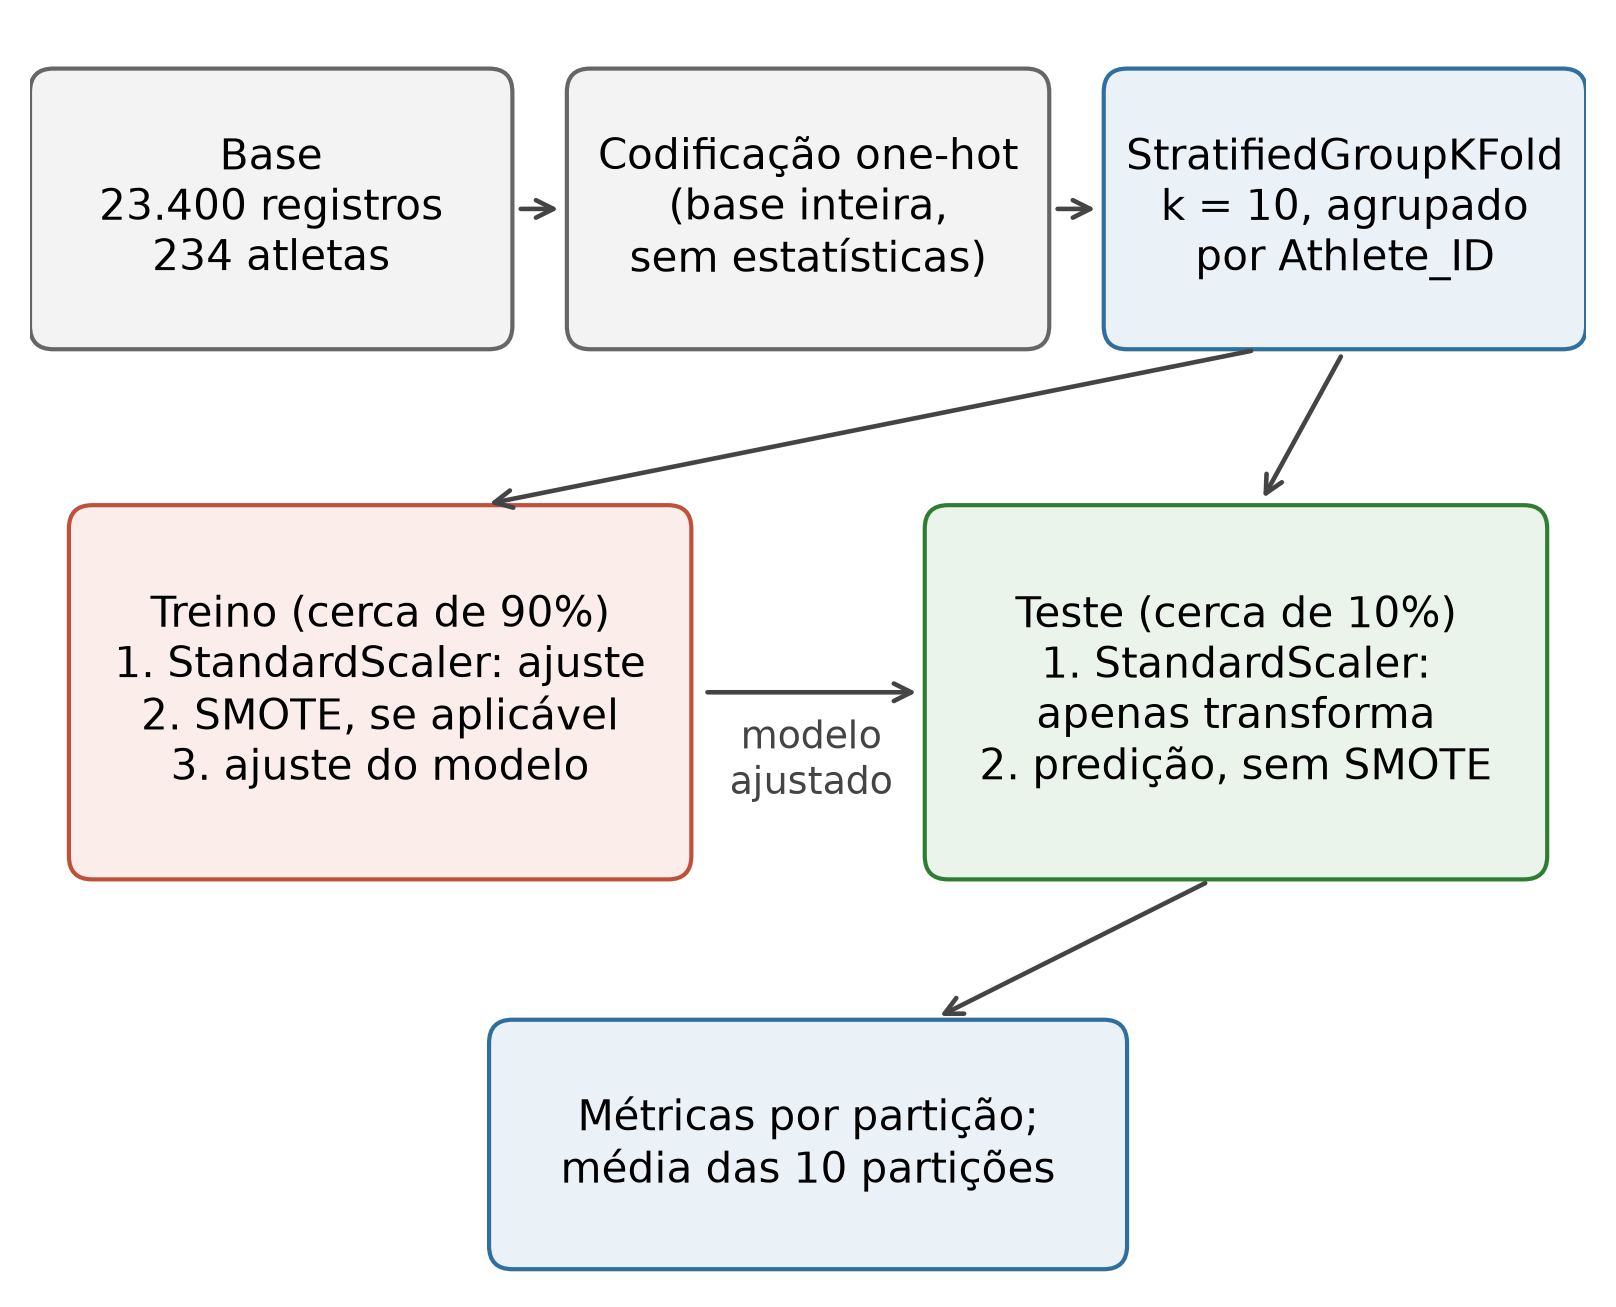
\includegraphics[width=\textwidth]{fig_leve/38_diagrama_pipeline_v3.png}
    \caption{Sequência de pré-processamento e validação.}
    \label{fig:pipeline}
\end{figure}

A figura mostra a sequência executada em cada uma das dez partições. A codificação \textit{one-hot} é aplicada uma única vez à base inteira, enquanto a padronização e o SMOTE são ajustados apenas na porção de treinamento. A porção de teste é somente transformada, com os parâmetros estimados no treinamento, e não recebe registros sintéticos.

O tratamento previsto para valores ausentes era imputação pela mediana nas variáveis numéricas e pela moda nas categóricas. A inspeção não identificou valores ausentes, de modo que nenhuma imputação foi efetivamente realizada.

\subsection{Hiperparâmetros}

A lista a seguir registra os hiperparâmetros definidos explicitamente para cada algoritmo. Os parâmetros não listados mantiveram os valores padrão das respectivas bibliotecas.

\begin{itemize}
    \item \texttt{DummyClassifier}: \texttt{strategy} igual a \texttt{most\_frequent} e a \texttt{stratified};
    \item \texttt{LogisticRegression}: \texttt{max\_iter = 1000};
    \item \texttt{DecisionTreeClassifier}: valores padrão, sem limite de profundidade;
    \item \texttt{RandomForestClassifier}: \texttt{n\_estimators = 200};
    \item \texttt{XGBClassifier}: \texttt{n\_estimators = 300}, \texttt{max\_depth = 6}, \texttt{learning\_rate = 0{,}1}, \texttt{subsample = 0{,}8}, \texttt{colsample\_bytree = 0{,}8}, \texttt{eval\_metric = logloss};
    \item \texttt{HistGradientBoostingClassifier}: \texttt{max\_iter = 300};
    \item \texttt{SMOTE}: \texttt{k\_neighbors = 5} e \texttt{sampling\_strategy} padrão, que iguala a classe minoritária à majoritária.
\end{itemize}

Nas configurações identificadas por \textit{Weights}, o parâmetro \texttt{class\_weight} recebeu o valor \texttt{balanced}. Na configuração \texttt{scale\_pos\_weight} do XGBoost, o valor empregado foi a razão entre o número de registros negativos e positivos, calculada uma única vez sobre o conjunto completo (17{,}04 na base completa e 17{,}82 no subconjunto de futebol), e não recalculada em cada partição. Como a validação é estratificada pela variável-alvo, essa razão varia pouco entre partições.

\subsection{Busca de Hiperparâmetros}
\label{sec:busca}

A busca sobre o \textit{Random Forest} empregou \texttt{RandomizedSearchCV} com 25 configurações amostradas, critério de seleção F1-Score e validação interna por \texttt{StratifiedGroupKFold} com $k = 3$, agrupada por atleta. O espaço de busca cobriu número de árvores, profundidade máxima, mínimo de amostras para divisão e para folha, número de atributos por divisão e ponderação de classes.

Cabe registrar explicitamente o desenho adotado, por afetar a interpretação do resultado. A busca foi conduzida uma única vez sobre o conjunto completo, e a configuração selecionada foi posteriormente avaliada por validação cruzada sobre esse mesmo conjunto. Não houve busca interna independente em cada partição externa. Em consequência, a escolha dos hiperparâmetros teve acesso a registros que depois compuseram as partições de avaliação, condição que, em princípio, favorece a configuração resultante.

Por esse motivo, a estimativa principal reportada para o \textit{Random Forest} otimizado é a da validação cruzada aninhada, na qual uma busca independente é executada sobre a porção de treinamento de cada partição externa. O desenho não aninhado é mantido apenas como comparação metodológica, na Seção~\ref{sec:boosting}.

Os modelos de \textit{gradient boosting} não foram submetidos a busca de hiperparâmetros, e foram avaliados na configuração indicada acima. A comparação entre eles e o \textit{Random Forest} otimizado é, portanto, assimétrica quanto ao esforço de ajuste.

\subsection{Métricas}

Acurácia, Precisão, Recall e F1-Score foram calculados pelas implementações de \texttt{sklearn.metrics}, com \texttt{zero\_division = 0}, convenção que atribui valor nulo à precisão quando o classificador não prediz nenhum positivo. A área sob a curva precisão-recall foi estimada por \texttt{average\_precision\_score} e é reportada como precisão média (AP), definida como a soma dos ganhos de recall entre limiares consecutivos ponderados pela precisão correspondente. Não se trata de integração trapezoidal da curva precisão-recall, procedimento que produziria valores ligeiramente distintos.

Todas as métricas foram calculadas por partição e posteriormente agregadas por média aritmética simples. Essa agregação difere do cálculo da métrica sobre o conjunto completo: razões calculadas em subconjuntos e depois promediadas não coincidem, em geral, com a razão calculada sobre a união dos subconjuntos. A diferença explica, por exemplo, que a regra apresente F1-Score de $0{,}1847$ quando avaliada sobre a base completa e $0{,}1833$ quando avaliada como média das dez partições. Por esse motivo, as comparações diretas com os modelos usam o segundo valor.

\subsection{Explicabilidade}
\label{sec:explic_metodo}

Os três métodos foram aplicados sobre um \textit{Random Forest} de 200 árvores com \texttt{class\_weight = balanced}, ajustado sobre a partição de treinamento do \textit{holdout} agrupado, e não sobre os modelos da validação cruzada. Trata-se, portanto, de um modelo distinto daqueles cujas métricas constam da Tabela~\ref{tab:resultados}, ainda que de mesma configuração.

A Importância de Gini foi extraída do atributo \texttt{feature\_importances\_} do modelo ajustado. A Importância por Permutação foi calculada sobre a partição de avaliação, com \texttt{scoring} igual a \texttt{roc\_auc} e 10 repetições por atributo. Os valores SHAP foram obtidos com \texttt{TreeExplainer}, sobre uma subamostra aleatória de 800 registros da partição de avaliação, com os atributos já padronizados; a subamostragem decorre do custo computacional do cálculo exato. Por ter sido sorteada sem estratificação, essa subamostra contém um único registro da região da regra, condição que afeta a leitura dos resultados, discutida na Seção~\ref{sec:shap}, e que confere ao resultado do SHAP caráter exploratório.

A árvore apresentada na Figura~\ref{fig:arvore} tem finalidade exclusivamente ilustrativa. Ela foi ajustada à parte, sobre o conjunto completo e sem padronização, de modo que os limiares apareçam nas unidades originais das variáveis, com profundidade máxima 4 e \texttt{class\_weight = balanced}. Por ter sido ajustada sobre todos os registros, não produz estimativa de desempenho e não corresponde a nenhum dos modelos avaliados nas tabelas de resultados.

% =====================================================================
% CAPÍTULO 5: RESULTADOS E DISCUSSÃO
% =====================================================================
% Quebra de página forçada no Sumário. Sem ela, a virada de página cai
% em cima das entradas 5.2.4 e 5.3, que desaparecem da listagem.
\addtocontents{toc}{\protect\newpage}
\chapter{RESULTADOS E DISCUSSÃO}
\label{cap:resultados}

Este capítulo apresenta os resultados obtidos e os discute à luz das limitações de cada análise. A exposição começa pela análise exploratória, que levou à identificação de uma regra associada ao rótulo, e segue para a comparação entre os modelos e para as técnicas de explicabilidade. Em seguida, examina o efeito do protocolo de validação sobre as métricas e encerra com a análise restrita aos registros de futebol.

\section{Análise Exploratória de Dados}

A análise exploratória examinou a distribuição da variável-alvo e a capacidade de cada variável em separar as classes. Desse exame resultou a identificação de uma regra associada ao rótulo, e a partir dela foram investigados o resíduo não abrangido pela regra e a referência de desempenho que ela fornece.

\subsection{Distribuição da Variável-Alvo}
O conjunto de dados apresenta um desbalanceamento severo: dos 23.400 registros, apenas 1.297 (5{,}54\%) pertencem à classe positiva (\texttt{Injury\_Risk = 1}), contra 22.103 (94{,}46\%) da classe negativa. Essa proporção de aproximadamente 17:1 configura um cenário onde a acurácia global é uma métrica enganosa, situação conhecida como Paradoxo da Acurácia. A Figura~\ref{fig:dist_target} ilustra essa assimetria.

\begin{figure}[H]
    \centering
    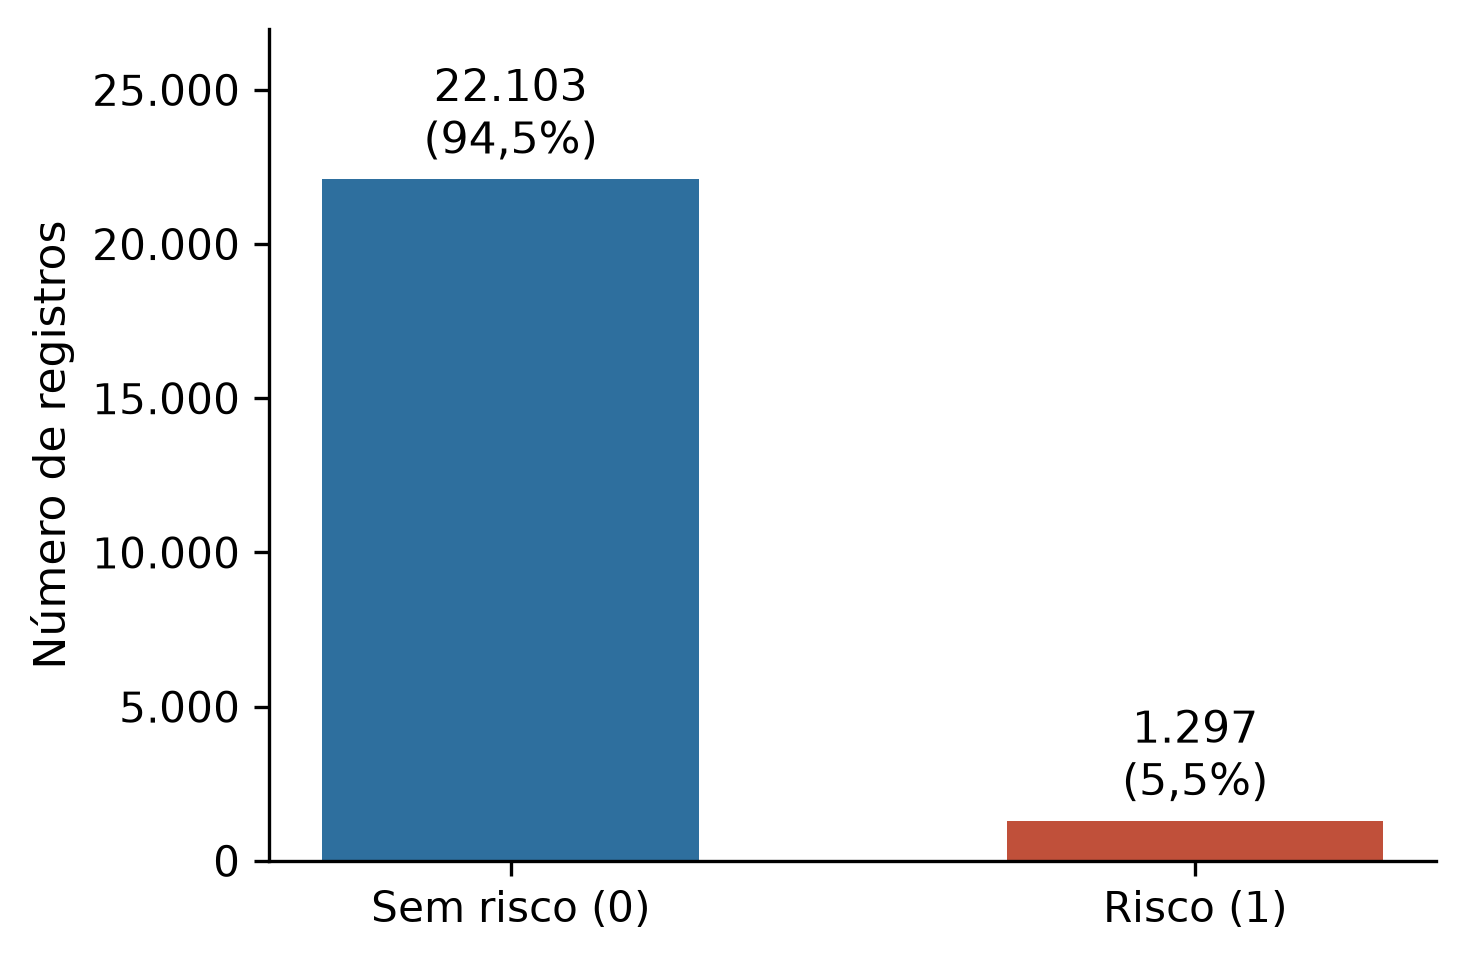
\includegraphics[width=0.75\textwidth]{fig_leve/26_distribuicao_alvo_v3.png}
    \caption{Distribuição da variável-alvo \texttt{Injury\_Risk}.}
    \label{fig:dist_target}
\end{figure}

\subsection{Poder Discriminante das Variáveis}
Para quantificar a capacidade de cada variável em separar as duas classes, foi calculado o $d$ de Cohen, uma medida padronizada de tamanho de efeito. A Tabela~\ref{tab:cohen_d} apresenta os resultados.

\begin{table}[H]
\centering
\caption{Tamanho de efeito ($d$ de Cohen) das variáveis numéricas.}
\label{tab:cohen_d}
\begin{tabular}{lrrr}
\toprule
Variável & Média (classe 0) & Média (classe 1) & $|d|$ \\
\midrule
Heart\_Rate         & 139{,}81 & 142{,}90 & 0{,}205 \\
Muscle\_Activity    & 49{,}99  & 50{,}29  & 0{,}029 \\
Oxygen\_Saturation  & 97{,}00  & 97{,}03  & 0{,}018 \\
Age                 & 23{,}53  & 23{,}59  & 0{,}017 \\
Motion\_Z           & 9{,}80   & 9{,}82   & 0{,}017 \\
Motion\_X           & 0{,}009  & $-$0{,}005 & 0{,}014 \\
Motion\_Y           & $-$0{,}004 & $-$0{,}001 & 0{,}003 \\
\bottomrule
\end{tabular}
\end{table}

Apenas \texttt{Heart\_Rate} apresentou um efeito pequeno ($|d| = 0{,}205$); todas as demais variáveis ficaram abaixo do limiar de 0{,}2 considerado negligível pela escala de Cohen, como se observa na Figura~\ref{fig:cohen_d}. Esse resultado antecipava que a separabilidade entre classes seria limitada.

\begin{figure}[H]
    \centering
    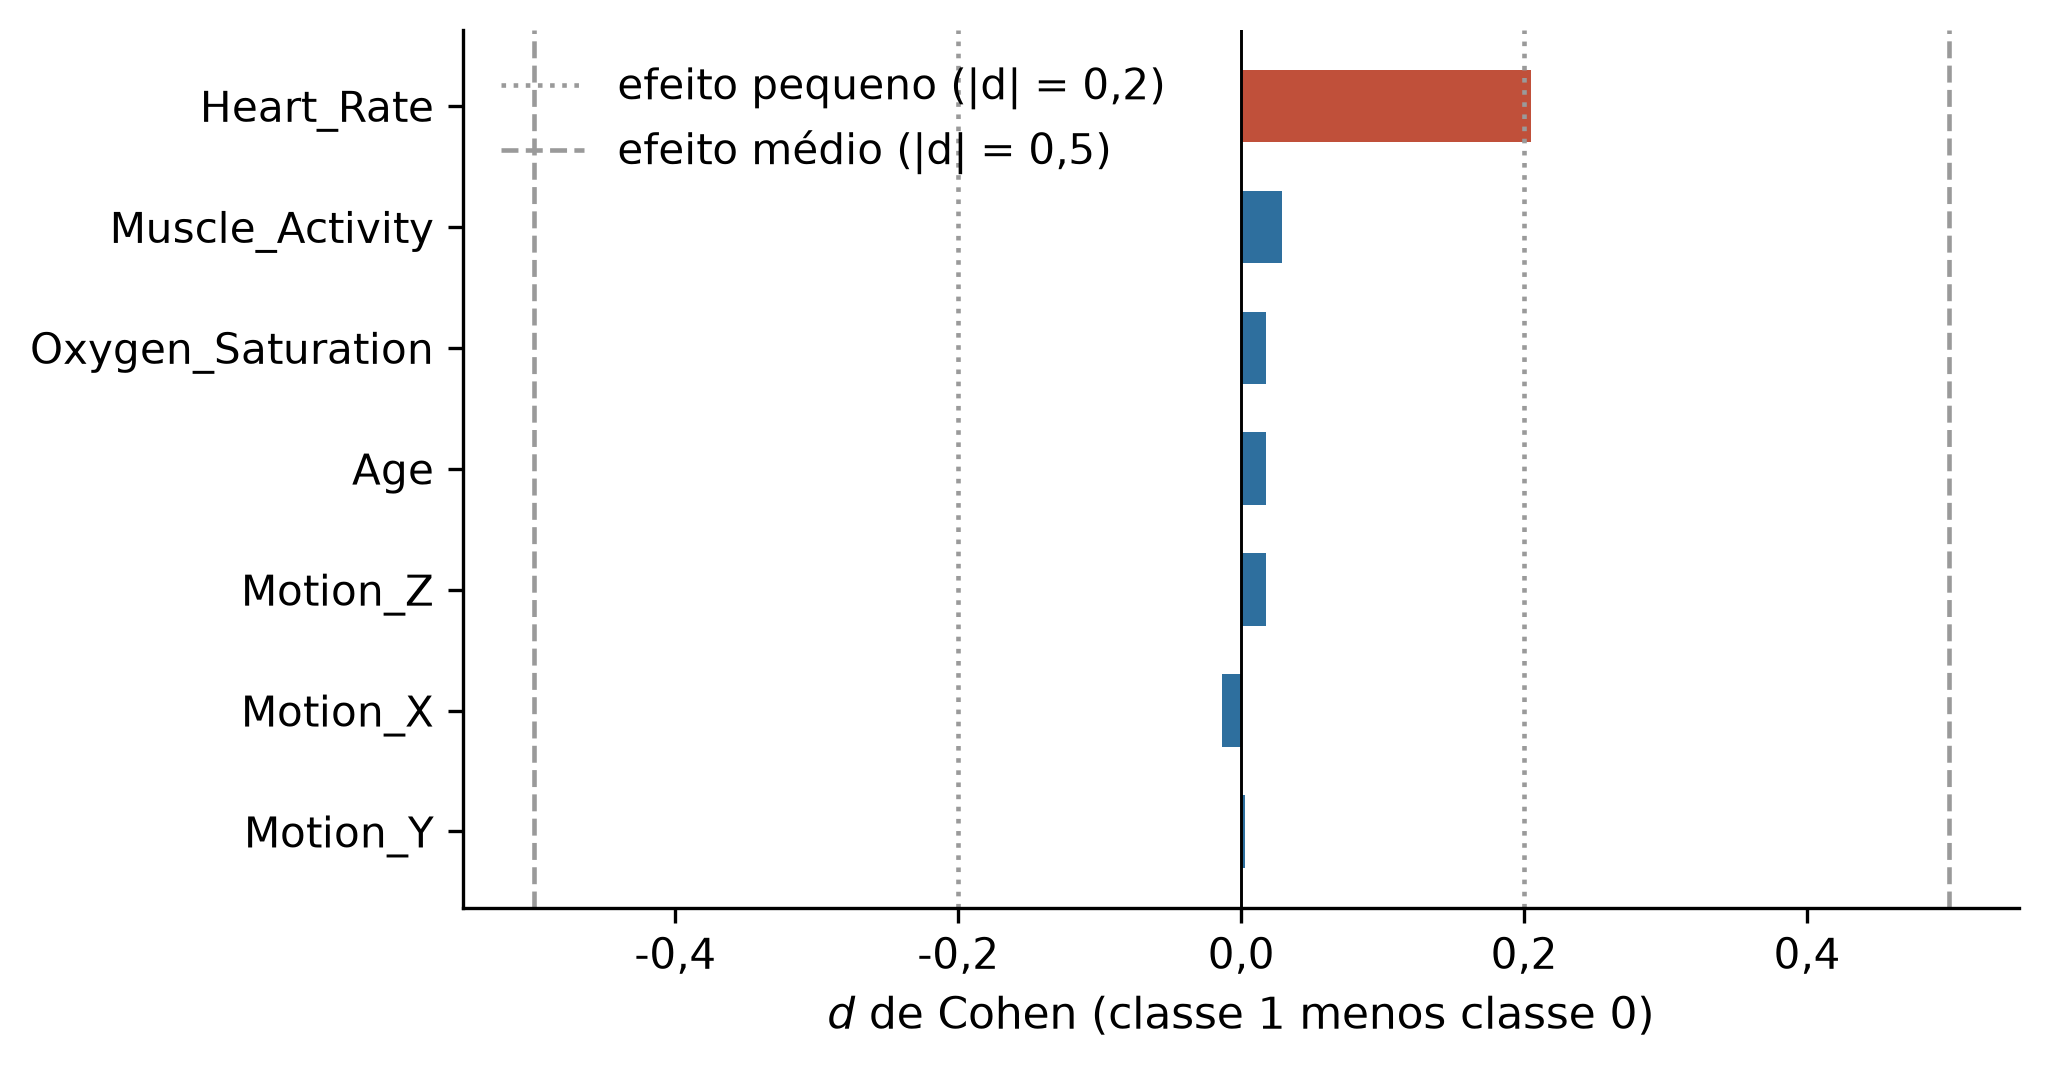
\includegraphics[width=\textwidth]{fig_leve/27_cohen_d_v3.png}
    \caption{Tamanho de efeito ($d$ de Cohen) por variável.}
    \label{fig:cohen_d}
\end{figure}

Na figura, o tamanho de efeito aparece com sinal: valores positivos indicam média maior na classe de risco, e negativos, média maior na classe sem risco. As linhas verticais marcam os limiares de efeito pequeno e médio da escala de Cohen, e apenas \texttt{Heart\_Rate} ultrapassa o primeiro deles.

\subsection{Identificação de uma Regra Compatível com os Rótulos}
\label{sec:regra}
A investigação do motivo pelo qual o \textit{Random Forest} atingia Precisão de exatamente 1{,}0000, isto é, nunca errava quando previa risco, levou à identificação de uma regra associada ao rótulo, obtida pelo procedimento de busca descrito a seguir. Para cada uma das sete variáveis numéricas da base, tomou-se o maior valor observado entre os registros da classe negativa. Em seguida, verificou-se se \textit{todos} os registros situados acima desse valor pertenciam à classe positiva. Duas variáveis satisfizeram essa condição, \texttt{Heart\_Rate} e \texttt{Muscle\_Activity}; as demais não apresentaram nenhum corte com essa propriedade. Os limiares, portanto, não foram arbitrados: decorrem diretamente do valor máximo observado na classe negativa de cada variável, respectivamente $179{,}979$ e $79{,}868$, referidos no texto de forma abreviada como 180 e 80. Os experimentos aplicam os cortes exatos; com os valores abreviados, a regra classifica os 23.400 registros da mesma forma, de modo que o arredondamento não altera nenhuma predição.

Quanto ao escopo dessa busca, foram examinados cortes univariados, uma variável de cada vez, e as duas condições encontradas foram combinadas por disjunção. Combinações conjuntivas, cortes envolvendo três ou mais variáveis e fronteiras não alinhadas aos eixos não foram exploradas, de modo que a regra identificada não é necessariamente a única descrição compatível com os dados.

Cabe registrar ainda que essa investigação utilizou a base completa, e não uma parte dos dados reservada para esse fim. A regra resultante é, portanto, uma descrição obtida na própria amostra, e não uma hipótese formulada de forma independente e posteriormente testada. Essa condição é retomada nas Seções~\ref{sec:oraculo} e~\ref{sec:regra_particoes}. A regra identificada é:

\begin{equation}
\label{eq:regra}
\texttt{Injury\_Risk} = 1 \quad \text{se} \quad (\texttt{Heart\_Rate} > 180) \;\lor\; (\texttt{Muscle\_Activity} > 80)
\end{equation}

Dos 23.400 registros, 132 satisfazem essa condição, e todos os 132 são positivos, sem nenhuma exceção. Esses 132 registros explicam 10{,}18\% dos 1.297 positivos totais. Os 1.165 positivos restantes (89{,}82\%) pertencem ao resíduo, região em que a proporção de positivos é de aproximadamente 5\%. A Figura~\ref{fig:regra} evidencia graficamente a separação imposta pela regra.

\begin{figure}[H]
    \centering
    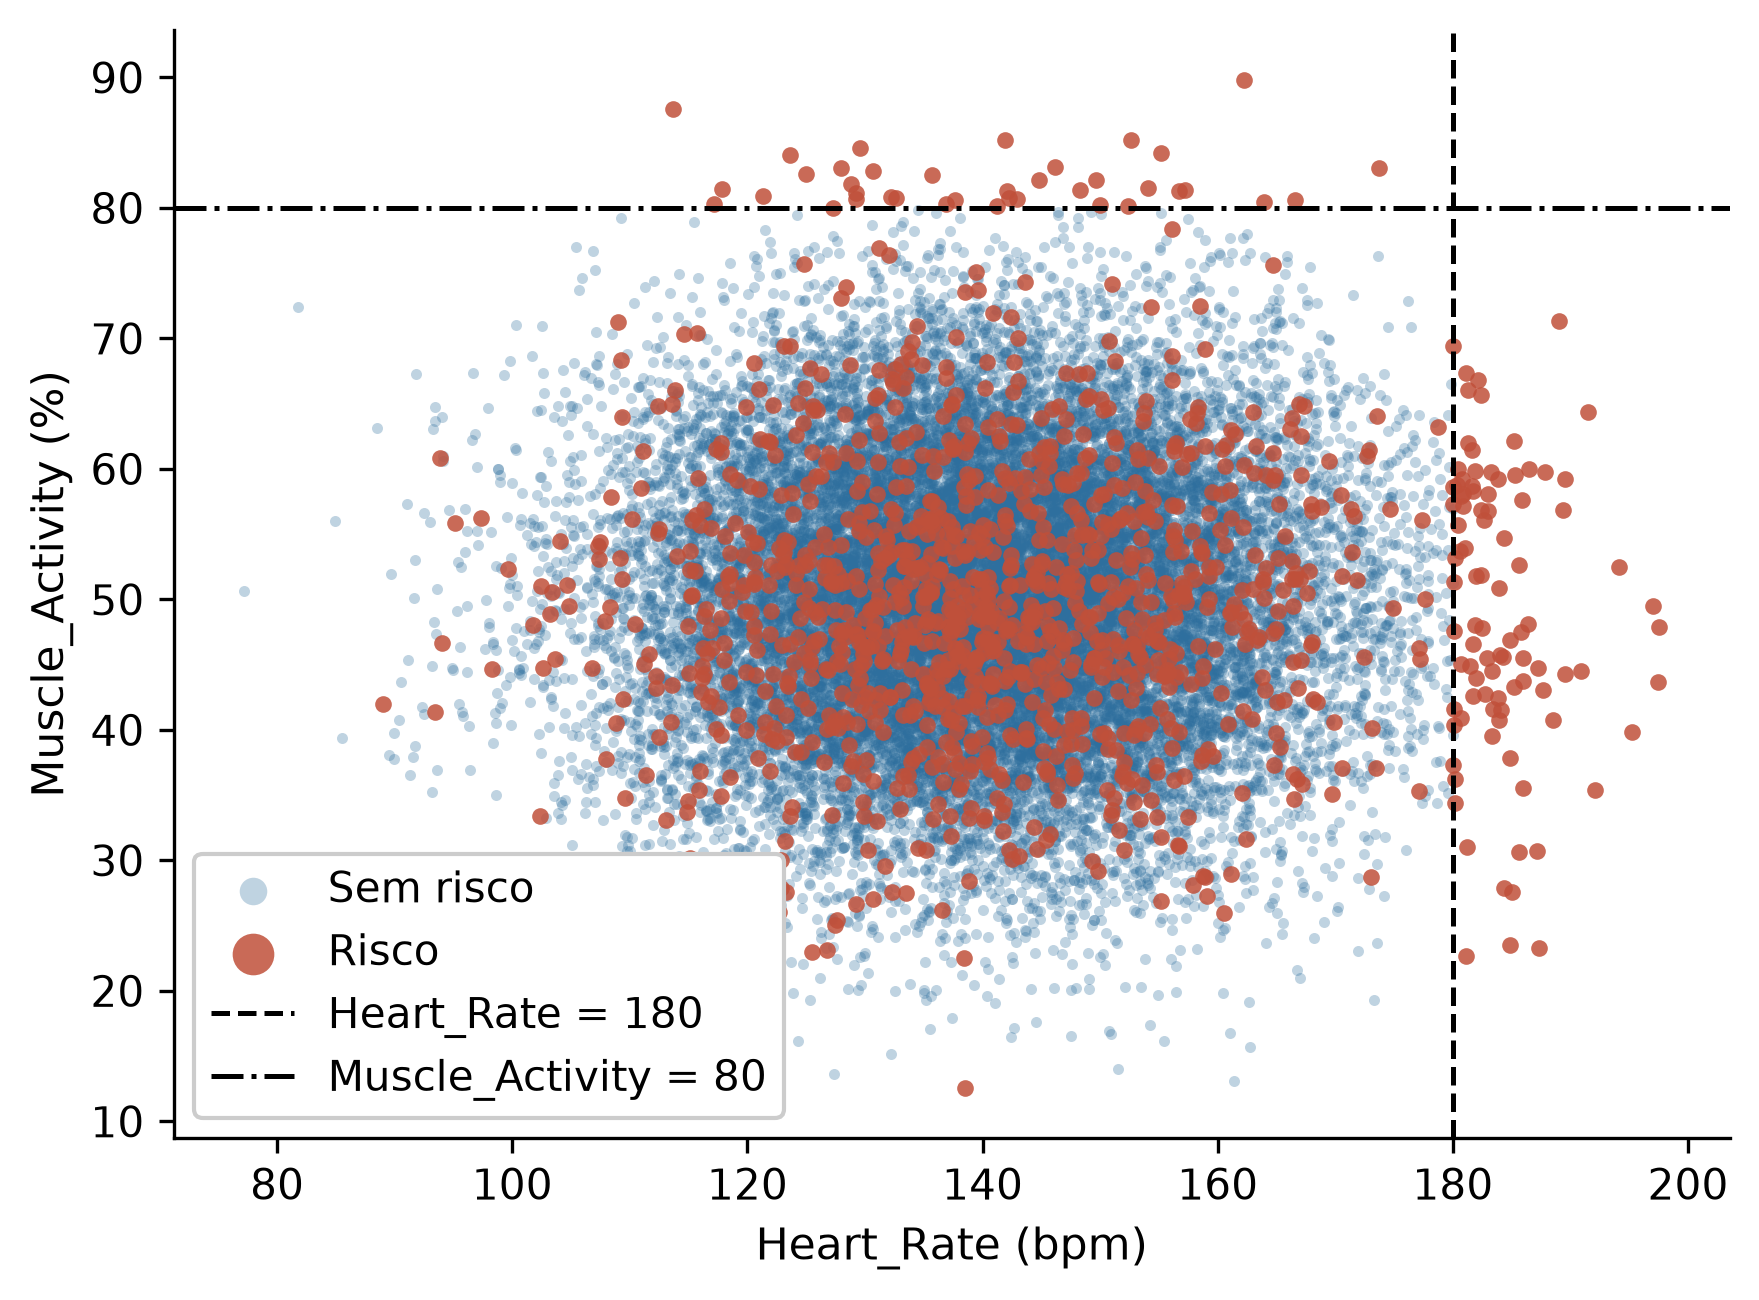
\includegraphics[width=\textwidth]{fig_leve/41_regra_deterministica_v3.png}
    \caption{Visualização da regra identificada.}
    \label{fig:regra}
\end{figure}

Cada ponto da figura é um registro, posicionado pela frequência cardíaca e pela atividade muscular. Todos os registros situados à direita da linha vertical, com $\texttt{Heart\_Rate} > 180$, ou acima da linha horizontal, com $\texttt{Muscle\_Activity} > 80$, pertencem à classe de risco. Abaixo e à esquerda dos dois cortes, as duas classes aparecem misturadas, sem separação visível.

A análise do resíduo oferece uma primeira indicação de que, nessa região, o rótulo não depende das variáveis medidas: o maior $|d|$ de Cohen entre os registros fora da regra é 0{,}064 (\texttt{Muscle\_Activity}), valor classificado como desprezível. Esse indicador, contudo, compara apenas médias, e médias semelhantes podem ocultar relações não lineares ou interações entre atributos. A Seção~\ref{sec:residuo} submete o resíduo a um teste mais exigente. Com base nessas evidências, formula-se a seguinte hipótese sobre a geração dos rótulos, que não pode ser confirmada sem acesso ao gerador original:

\begin{equation}
\texttt{Injury\_Risk} =
\begin{cases}
1, & \text{se } \texttt{Heart\_Rate} > 180 \;\lor\; \texttt{Muscle\_Activity} > 80 \\
\text{Bernoulli}(0{,}0501), & \text{caso contrário}
\end{cases}
\end{equation}

\subsection{Investigação de Sinal Preditivo Fora da Regra}
\label{sec:residuo}

Para submeter o resíduo a um teste mais exigente que o tamanho de efeito, os 23.268 registros não abrangidos pela regra foram isolados, e sobre eles foi treinado e avaliado um \textit{Random Forest} de 200 árvores, sob o mesmo protocolo de validação cruzada agrupada por atleta empregado no restante do experimento. A escolha do algoritmo é deliberada: florestas de decisão capturam exatamente as relações não lineares e as interações entre atributos que o tamanho de efeito não consegue descartar. Se existisse estrutura aprendível no resíduo, este seria o procedimento com maior chance de encontrá-la. A Tabela~\ref{tab:residuo} reúne as médias e os desvios-padrão obtidos nas dez partições, ao lado do valor que cada métrica assumiria para um classificador sem sinal.

\begin{table}[H]
\centering
\caption{Desempenho de um classificador restrito ao resíduo.}
\label{tab:residuo}
\begin{tabular}{lrrr}
\toprule
Métrica & Média & Desvio-padrão & Referência do acaso \\
\midrule
Precisão  & 0{,}0000 & 0{,}0000 & 0{,}0501 \\
Recall    & 0{,}0000 & 0{,}0000 & -- \\
F1-Score  & 0{,}0000 & 0{,}0000 & -- \\
ROC-AUC   & 0{,}4951 & 0{,}0210 & 0{,}5000 \\
AP        & 0{,}0506 & 0{,}0034 & 0{,}0501 \\
\bottomrule
\end{tabular}
\end{table}

Os dois indicadores invariantes ao limiar de decisão são os que importam nesta leitura. A ROC-AUC obtida, $0{,}4951 \pm 0{,}0210$, é indistinguível do valor esperado para uma ordenação aleatória, $0{,}5000$. A precisão média, $0{,}0506 \pm 0{,}0034$, fica próxima da proporção de positivos no resíduo, $0{,}0501$, que é o valor esperado dessa métrica para um classificador sem sinal. Precisão, recall e F1-Score são nulos porque o modelo não atribuiu a classe positiva a nenhum registro, comportamento esperado quando nenhuma região do espaço de atributos concentra positivos.

Cabe delimitar o que esse resultado autoriza concluir. Ele não demonstra que os rótulos do resíduo foram efetivamente sorteados, afirmação que exigiria acesso ao procedimento gerador original, indisponível. O que ele estabelece é que um algoritmo capaz de representar relações não lineares e interações, submetido a um protocolo de validação que impede a sobreposição de atletas entre treino e avaliação, não identificou sinal preditivo consistente nessa região. Esse achado é compatível com a presença de uma componente aleatória na rotulagem, e é sob essa condição que os resultados das seções seguintes devem ser lidos.

\subsection{Referência de Desempenho Derivada da Regra}
\label{sec:limite}

Dois indicadores são usados ao longo deste capítulo para avaliar os classificadores, e convém defini-los antes de prosseguir. A Precisão responde à pergunta: das vezes em que o classificador apontou risco, quantas estavam corretas? O Recall, também chamado de sensibilidade, responde à pergunta complementar: do total de casos de risco existentes, quantos o classificador encontrou? O F1-Score combina os dois em um único número, por meio da média harmônica, e só é alto quando ambos são altos simultaneamente. Um classificador que aponte risco raramente, mas sempre acerte, terá precisão alta e recall baixo, e o F1-Score refletirá esse desequilíbrio.

Aplicando a regra da Equação~\ref{eq:regra} diretamente sobre a base, sem treinar classificador algum, obtém-se precisão $1{,}0000$, recall $132 / 1297 = 0{,}1018$ e F1-Score $0{,}1847$. A precisão é máxima porque a regra nunca falha: os 132 registros que ela seleciona são todos positivos. O recall é baixo porque a regra alcança apenas 10{,}18\% das ocorrências de risco, já que as demais estão fora da região que ela abrange.

O valor $0{,}1018$, contudo, não é o recall máximo possível nesta base. Um classificador que apontasse risco para todos os 23.400 registros alcançaria recall $1{,}0000$, embora com precisão de apenas $0{,}0554$ e F1-Score de $0{,}1050$. O valor $0{,}1018$ é o recall \textit{da regra}, e corresponde ao ponto em que o F1-Score é maximizado.

Para verificar essa afirmação sem recorrer a dedução, foi calculado o desempenho de classificadores hipotéticos que, além dos 132 registros da regra, também apontam risco para $k$ registros escolhidos ao acaso no resíduo. A Tabela~\ref{tab:varredura} apresenta o resultado, calculado sobre a base completa, em função de quantos registros do resíduo são adicionalmente apontados como risco.

\begin{table}[H]
\centering
\caption{Desempenho ao apontar parte do resíduo.}
\label{tab:varredura}
\begin{tabular}{rrrr}
\toprule
$k$ & Precisão & Recall & F1-Score \\
\midrule
0 (apenas a regra) & 1{,}0000 & 0{,}1018 & 0{,}1847 \\
100                & 0{,}5905 & 0{,}1056 & 0{,}1792 \\
500                & 0{,}2485 & 0{,}1211 & 0{,}1628 \\
1.000              & 0{,}1608 & 0{,}1404 & 0{,}1499 \\
5.000              & 0{,}0745 & 0{,}2948 & 0{,}1189 \\
10.000             & 0{,}0624 & 0{,}4878 & 0{,}1107 \\
23.268 (todos)     & 0{,}0554 & 1{,}0000 & 0{,}1050 \\
\bottomrule
\end{tabular}
\end{table}

O F1-Score é máximo em $k = 0$ e decresce de forma monotônica. A razão é direta: no resíduo a taxa de acerto é de aproximadamente 5\%, contra 100\% entre os registros da regra. Cada registro adicionalmente apontado dilui a precisão mais do que contribui para o recall. O valor $0{,}1847$ constitui, portanto, uma referência descritiva de desempenho da regra na base completa.

Os modelos, contudo, são avaliados como média de dez partições, e uma razão calculada em cada partição e depois promediada não coincide, em geral, com a mesma razão calculada sobre a base inteira. Aplicada às mesmas dez partições usadas pelos modelos, a regra obtém F1-Score médio de $0{,}1833$, e é esse o valor usado nas comparações diretas com os modelos nas seções seguintes.

Essa referência é condicionada, e a condição precisa ser explicitada. A varredura da Tabela~\ref{tab:varredura} supõe que os registros adicionalmente apontados sejam escolhidos \textit{ao acaso} dentro do resíduo, suposição que se apoia no resultado da Seção~\ref{sec:residuo}: um classificador não linear, sob validação agrupada, não identificou sinal preditivo naquela região. Caso existisse estrutura ali que os procedimentos empregados não tenham detectado, um classificador capaz de explorá-la poderia superar o valor. O que os experimentos autorizam afirmar é que a regra identificada fornece uma referência descritiva, válida sob a hipótese de ausência de sinal no resíduo, e não um limite universal demonstrado para qualquer classificador.

\section{Resultados da Modelagem}

Esta seção compara o desempenho das configurações avaliadas e o confronta com a regra identificada na análise exploratória. Em seguida, a descoberta da regra é repetida dentro das partições, a conclusão é submetida a um teste de robustez com outros algoritmos e com busca de hiperparâmetros, e examina-se o efeito do ajuste de limiar.

\subsection{Comparação entre Modelos e Estratégias}

A Tabela~\ref{tab:resultados} apresenta os resultados consolidados das 11 configurações avaliadas (4 modelos $\times$ 3 estratégias de desbalanceamento, menos combinações redundantes), ordenados por F1-Score. Os valores foram obtidos por validação cruzada agrupada por atleta com $k = 10$, e para Recall, F1-Score e AP reporta-se a média $\pm$ o desvio-padrão entre as partições.

\begin{table}[H]
\centering
\caption{Resultados comparativos das 11 configurações.}
\label{tab:resultados}
\resizebox{\textwidth}{!}{%
\begin{tabular}{lrrcrcc}
\toprule
Configuração & Acurácia & Precisão & Recall & ROC-AUC & F1-Score & AP \\
\midrule
{[}Baseline{]} Random Forest       & 0{,}9502 & 1{,}0000          & $0{,}1014 \pm 0{,}0246$ & 0{,}5475 & $0{,}1833 \pm 0{,}0401$ & $0{,}1673 \pm 0{,}0273$ \\
{[}Weights{]} RF                   & 0{,}9502 & 1{,}0000          & $0{,}1006 \pm 0{,}0262$ & 0{,}5488 & $0{,}1818 \pm 0{,}0430$ & $0{,}1666 \pm 0{,}0282$ \\
{[}SMOTE{]} RF                     & 0{,}9313 & 0{,}2492          & $0{,}1144 \pm 0{,}0332$ & 0{,}5497 & $0{,}1549 \pm 0{,}0409$ & $0{,}1504 \pm 0{,}0319$ \\
{[}Weights{]} DT                   & 0{,}9023 & 0{,}1408          & $0{,}1500 \pm 0{,}0296$ & 0{,}5482 & $0{,}1451 \pm 0{,}0257$ & $0{,}0689 \pm 0{,}0062$ \\
{[}Baseline{]} Árvore de Decisão   & 0{,}8948 & 0{,}1239          & $0{,}1473 \pm 0{,}0300$ & 0{,}5430 & $0{,}1344 \pm 0{,}0273$ & $0{,}0662 \pm 0{,}0061$ \\
{[}SMOTE{]} DT                     & 0{,}8701 & 0{,}0972          & $0{,}1623 \pm 0{,}0331$ & 0{,}5370 & $0{,}1214 \pm 0{,}0230$ & $0{,}0628 \pm 0{,}0049$ \\
{[}SMOTE{]} LR                     & 0{,}5393 & 0{,}0594          & $0{,}4928 \pm 0{,}0551$ & 0{,}5244 & $0{,}1060 \pm 0{,}0113$ & $0{,}1072 \pm 0{,}0264$ \\
{[}Weights{]} LR                   & 0{,}5374 & 0{,}0591          & $0{,}4913 \pm 0{,}0467$ & 0{,}5252 & $0{,}1055 \pm 0{,}0112$ & $0{,}1054 \pm 0{,}0265$ \\
{[}Baseline{]} Dummy (Estrat.)     & 0{,}8952 & 0{,}0602          & $0{,}0610 \pm 0{,}0221$ & 0{,}5026 & $0{,}0606 \pm 0{,}0216$ & $0{,}0562 \pm 0{,}0017$ \\
{[}Baseline{]} Regressão Logística & 0{,}9446 & 0{,}0000          & $0{,}0000 \pm 0{,}0000$ & 0{,}5275 & $0{,}0000 \pm 0{,}0000$ & $0{,}1148 \pm 0{,}0289$ \\
{[}Baseline{]} Dummy (Majoritário) & 0{,}9446 & 0{,}0000          & $0{,}0000 \pm 0{,}0000$ & 0{,}5000 & $0{,}0000 \pm 0{,}0000$ & $0{,}0554 \pm 0{,}0011$ \\
\bottomrule
\end{tabular}%
}
\end{table}

A Figura~\ref{fig:comparativo} apresenta a mesma comparação em forma gráfica. Ela evidencia que as configurações de maior recall, as de Regressão Logística com ponderação de classes ou SMOTE, não são as de maior F1-Score.

\begin{figure}[H]
    \centering
    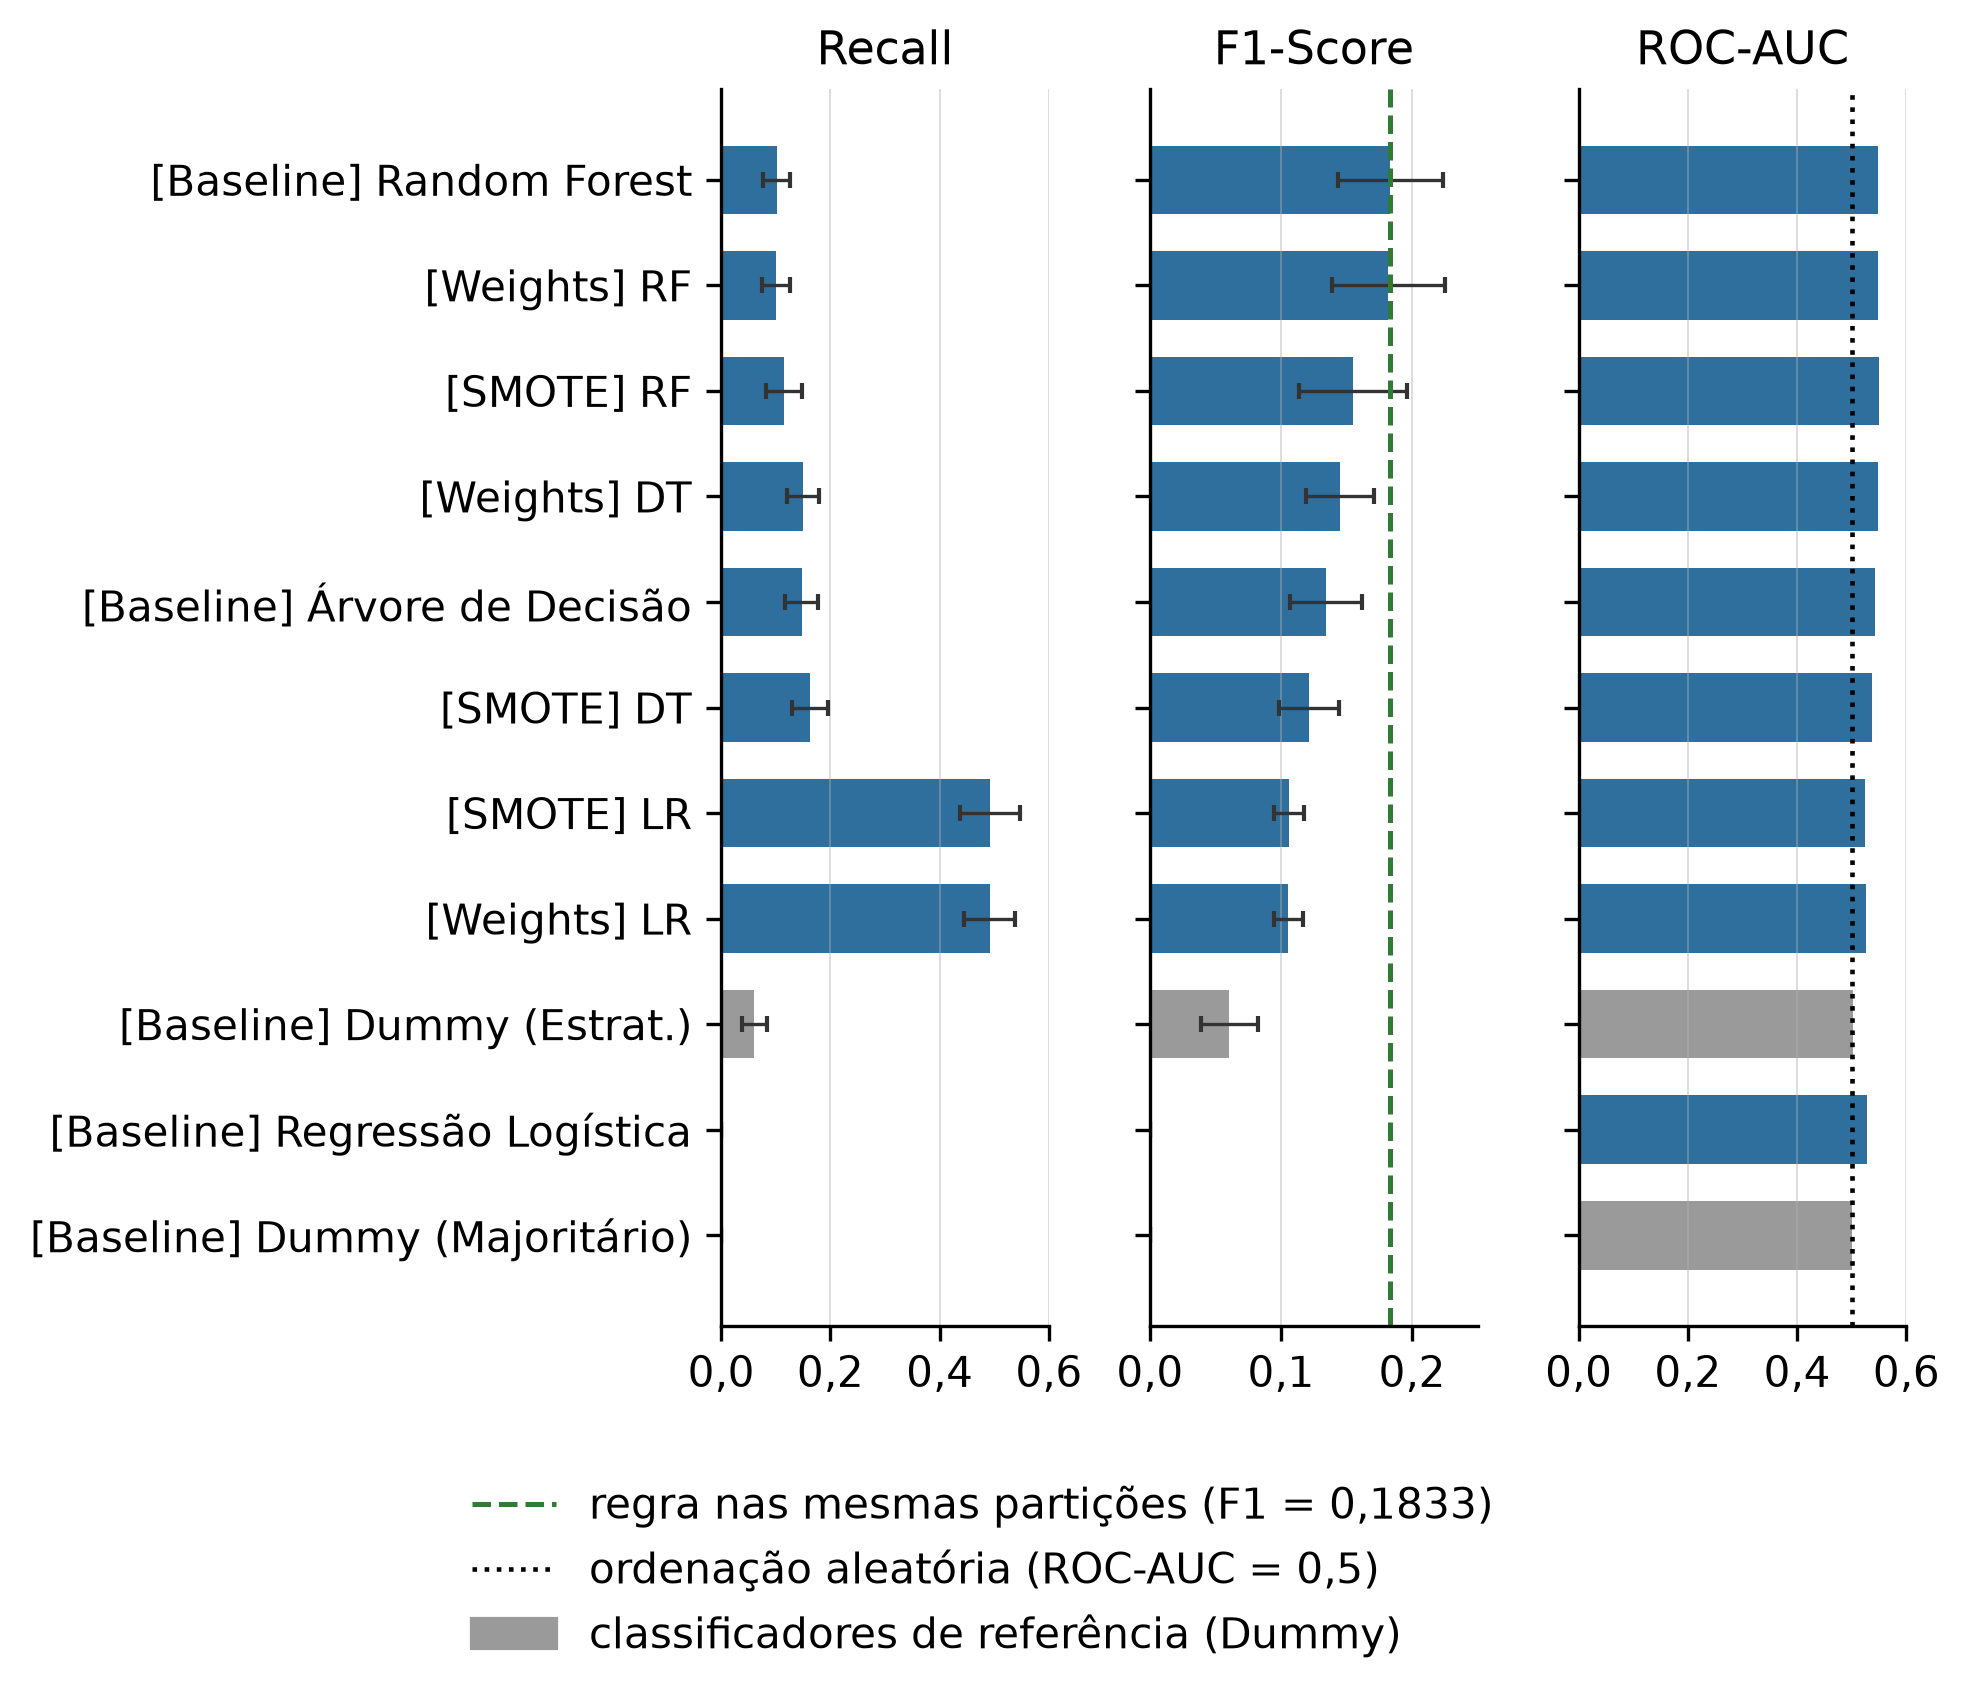
\includegraphics[width=\textwidth]{fig_leve/34_comparativo_metricas_v3.png}
    \caption{Recall, F1-Score e ROC-AUC por configuração.}
    \label{fig:comparativo}
\end{figure}

As configurações aparecem na mesma ordem da Tabela~\ref{tab:resultados}, e as hastes indicam o desvio-padrão entre partições. No painel central, a linha tracejada marca o F1-Score médio da regra nas mesmas partições, 0{,}1833, e no painel da direita a linha pontilhada marca o valor 0{,}5 da ROC-AUC, correspondente a uma ordenação aleatória.

O \textit{Random Forest} na configuração \textit{baseline}, isto é, sem tratamento de desbalanceamento, obteve o melhor F1-Score (0{,}1833) com Precisão de 1{,}0000. Isso significa que, quando o modelo previa ``risco'', acertava em todas as ocasiões, mas encontrava apenas 10{,}14\% dos casos reais de risco. Esse comportamento é consistente com a regra da Equação~\ref{eq:regra}: o modelo aponta risco somente na região que ela delimita, o que é verificado registro a registro na Seção~\ref{sec:oraculo}.

Convém observar a dispersão antes de extrair conclusões dessa ordenação. Os desvios-padrão entre partições são da ordem de $0{,}04$ para as três configurações de \textit{Random Forest}, enquanto as diferenças de F1-Score entre elas são de $0{,}0015$ e $0{,}0284$. As duas primeiras posições, portanto, não se distinguem diante da variação entre partições, e a leitura que se sustenta é a de agrupamento por família de algoritmo, e não a de um ordenamento fino entre configurações próximas.

A Regressão Logística \textit{baseline} e o Dummy Majoritário compartilham F1 = 0{,}0000, pois nunca previram a classe positiva. O classificador linear não encontrou fronteira de decisão que justificasse prever ``risco''.

\subsection{A Regra como Classificador de Referência}
\label{sec:oraculo}

A comparação entre o desempenho observado e a referência estabelecida na Seção~\ref{sec:limite} pode ser feita de forma direta, sem recorrer a nenhum cálculo intermediário. Basta implementar a regra da Equação~\ref{eq:regra} como um classificador e submetê-la ao mesmo protocolo de avaliação aplicado aos demais modelos.

Esse classificador não possui parâmetros e não passa por treinamento. Ele simplesmente responde ``risco'' quando a frequência cardíaca excede 180 batimentos por minuto ou a atividade muscular excede 80\%, e ``sem risco'' em qualquer outro caso. Avaliá-lo sobre as mesmas partições usadas pelos modelos treinados permite comparar diretamente o que a regra entrega com o que os algoritmos conseguem aprender. A Tabela~\ref{tab:oraculo} apresenta o resultado, comparando a regra ao melhor modelo treinado, com médias das dez partições agrupadas por atleta.

\begin{table}[H]
\centering
\caption{A regra como classificador de referência.}
\label{tab:oraculo}
\begin{tabular}{lrrr}
\toprule
Classificador & Precisão & Recall & F1-Score \\
\midrule
Regra aplicada diretamente      & 1{,}0000 & 0{,}1014 & 0{,}1833 \\
\textit{Random Forest} treinado & 1{,}0000 & 0{,}1014 & 0{,}1833 \\
\addlinespace
Apontar risco sempre            & 0{,}0554 & 1{,}0000 & 0{,}1050 \\
\bottomrule
\end{tabular}
\end{table}

Os dois primeiros resultados são idênticos nas três métricas. A coincidência de métricas, contudo, não garante por si só que as predições sejam as mesmas, já que valores arredondados podem ocultar divergências pontuais. Para verificar a equivalência no nível do registro, as predições do \textit{Random Forest} obtidas fora da amostra, sob o mesmo protocolo agrupado, foram comparadas uma a uma com a saída da regra: as duas coincidem em 23.400 dos 23.400 registros, sem nenhuma divergência. O modelo treinado reproduz a regra identificada, e não apenas o seu desempenho agregado.

Essa comparação tem, contudo, uma limitação importante: a regra foi identificada por meio da inspeção da base completa, e não a partir de uma parte dos dados reservada para esse fim. Sua aplicação posterior às mesmas partições não constitui, portanto, confirmação independente: trata-se de uma referência descritiva obtida na própria amostra, e os valores devem ser lidos sob essa condição. A Seção~\ref{sec:regra_particoes} examina essa limitação repetindo a descoberta apenas com os atletas de treinamento de cada partição. A terceira linha serve de contraste e confirma o que foi discutido na Seção~\ref{sec:limite}: é possível alcançar recall máximo apontando risco indiscriminadamente, ao custo de uma precisão de 5{,}54\% e de um F1-Score substancialmente inferior. A Figura~\ref{fig:teto} situa visualmente cada configuração avaliada em relação a essa referência.

\begin{figure}[H]
    \centering
    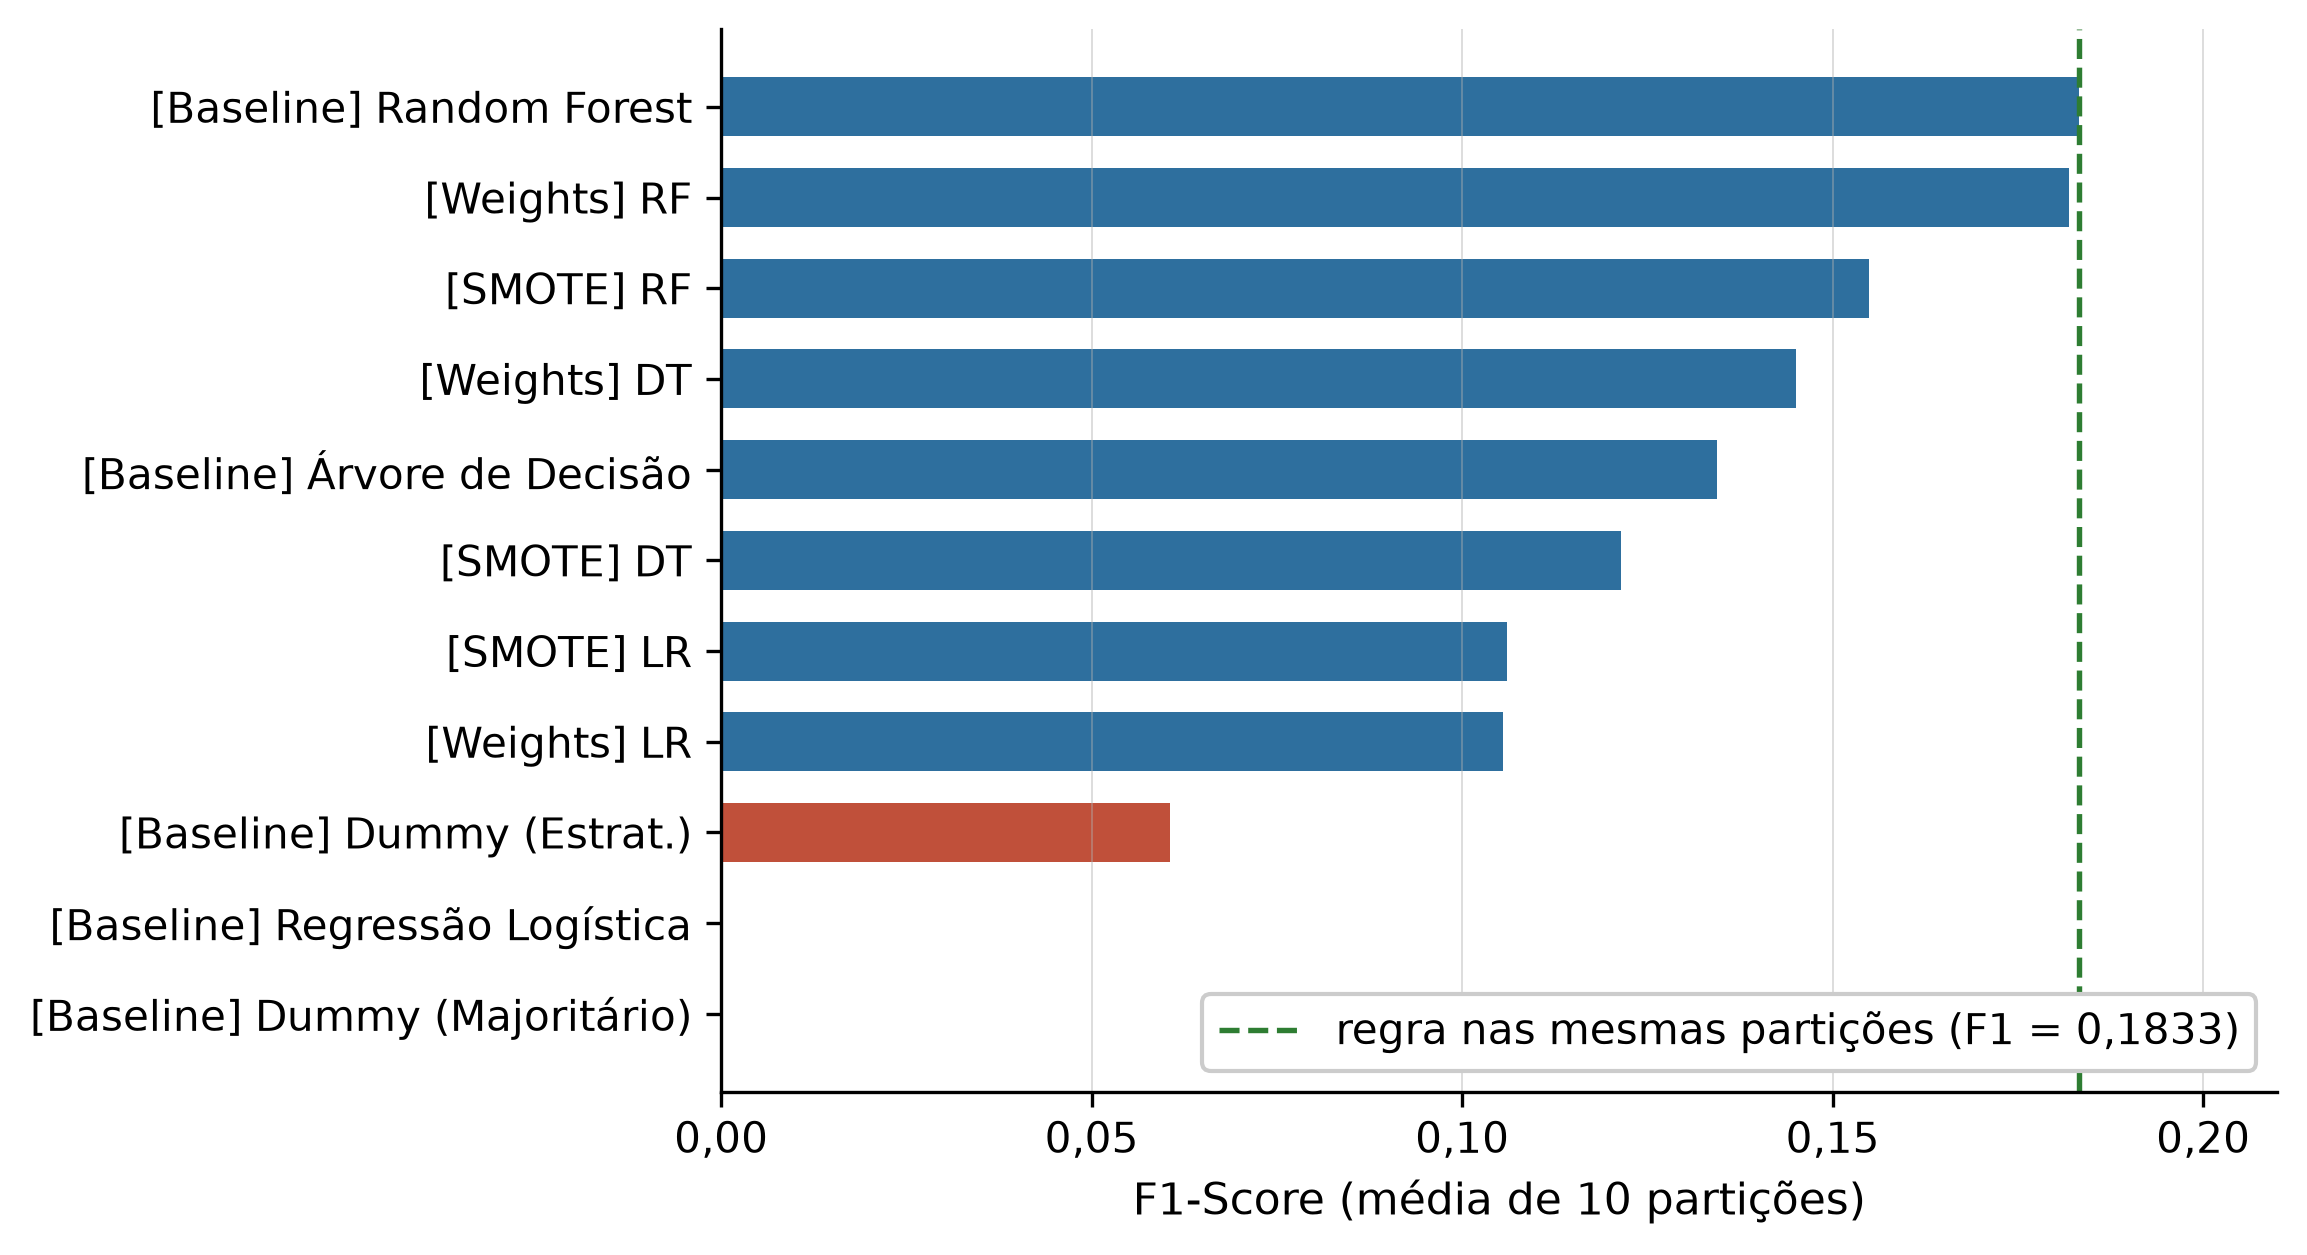
\includegraphics[width=\textwidth]{fig_leve/35_referencia_desempenho_v3.png}
    \caption{F1-Score por configuração e a referência da regra.}
    \label{fig:teto}
\end{figure}

Na figura, a linha tracejada corresponde ao F1-Score médio da regra identificada nas mesmas dez partições, 0{,}1833, e nenhuma configuração a ultrapassa. Esse resultado reorienta a leitura do experimento: o desempenho baixo dos melhores modelos não indica que tenham falhado em aprender, pois eles reproduziram integralmente a única estrutura que as análises conduzidas identificaram na base. Nesta base, o desempenho observado é limitado pelo procedimento que atribuiu os rótulos, e não pela capacidade dos algoritmos avaliados.

\subsection{Estabilidade da Regra em Atletas de Teste}
\label{sec:regra_particoes}

A limitação apontada na seção anterior pode ser examinada diretamente. Em vez de identificar a regra na base completa, o procedimento de descoberta foi repetido em cada uma das dez partições usando apenas os atletas de treinamento, e a regra obtida foi aplicada aos atletas de teste da mesma partição, que não participaram da descoberta.

O critério foi estendido em relação ao da Seção~\ref{sec:regra}. Para cada variável numérica foram examinadas as duas direções: acima do maior valor e abaixo do menor valor observado na classe negativa do treinamento. Um corte é aceito se houver um número mínimo de registros de treinamento além dele e se todos forem positivos. A regra resultante é a disjunção dos cortes aceitos. O experimento foi executado com dois valores para esse suporte mínimo, um e cinco registros, e ambos são reportados. A Tabela~\ref{tab:regra_particoes} resume o resultado com suporte de cinco registros, para a regra descoberta com os atletas de treinamento e aplicada aos atletas de teste, com médias das dez partições.

\begin{table}[H]
\centering
\caption{Regra descoberta no treinamento de cada partição.}
\label{tab:regra_particoes}
\resizebox{\textwidth}{!}{%
\begin{tabular}{lrr}
\toprule
 & Base completa & Subconjunto: futebol \\
\midrule
Partições com cortes em \texttt{Heart\_Rate} e \texttt{Muscle\_Activity} & 10 de 10 & 10 de 10 \\
Outros cortes encontrados & nenhum & nenhum \\
Corte em \texttt{Heart\_Rate} (mínimo a máximo) & 179{,}969 a 179{,}979 & 179{,}468 a 179{,}979 \\
Corte em \texttt{Muscle\_Activity} (mínimo a máximo) & 79{,}722 a 79{,}868 & 79{,}208 a 79{,}868 \\
Registros apontados no teste & 134 & 40 \\
Exceções no teste & 2 & 4 \\
Precisão média & 0{,}9845 & 0{,}9214 \\
F1-Score médio & $0{,}1831 \pm 0{,}0402$ & $0{,}2272 \pm 0{,}1052$ \\
F1-Score da regra fixada na base completa & 0{,}1833 & 0{,}2299 \\
Predições iguais às da regra fixada & 23.398 de 23.400 & 5.096 de 5.100 \\
\bottomrule
\end{tabular}%
}
\end{table}

Nas dez partições, a descoberta feita sem acesso aos atletas de teste recuperou as mesmas duas variáveis. Na base completa, o corte de frequência cardíaca variou de 179{,}969 a 179{,}979 bpm, e o de atividade muscular, de 79{,}722\% a 79{,}868\%. Aplicada aos atletas de teste, a regra obtida teve F1-Score médio de 0{,}1831, praticamente igual ao da regra fixada na base completa, e coincidiu com ela em 23.398 dos 23.400 registros. As exceções surgem nas partições em que registros negativos com os maiores valores de uma das variáveis ficaram no teste. O corte estimado no treinamento fica então ligeiramente abaixo, e esses registros passam a ser apontados como risco. É o comportamento esperado de um corte estimado com menos dados.

Com suporte mínimo de um registro, a busca encontrou ainda um terceiro corte, \texttt{Muscle\_Activity} abaixo de 13{,}03, em nove das dez partições. Esse corte é sustentado por um único registro, o de menor atividade muscular de toda a base, que é positivo. Com cerca de 5\% de positivos fora da regra, é esperado que um registro extremo isolado pertença à classe positiva por acaso. O corte desaparece quando se exige um mínimo de cinco registros. Ele afetou um único registro de teste, negativo, e o F1-Score médio passou a 0{,}1829. O episódio ilustra uma fragilidade do critério: cortes sustentados por pouquíssimos registros podem refletir acaso, e a busca original, restrita à direção acima do máximo, não teria como detectá-los.

Esse resultado, porém, tem alcance delimitado: mostra que o procedimento de descoberta é estável quando aplicado a atletas que não participaram dela, mas a verificação continua restrita à mesma base, cujas partições provêm todas do mesmo gerador. A confirmação em dados de outra procedência permanece fora do alcance deste trabalho.

% O titulo curto entre colchetes vale so para o Sumario e impede que
% HIPERPARAMETROS seja quebrado com hifen na virada da linha.
\subsection[Teste de Robustez: Gradient Boosting e Busca de \mbox{HIPERPARÂMETROS}]{Teste de Robustez: Gradient Boosting e Busca de Hiperparâmetros}
\label{sec:boosting}

A leitura de que o desempenho observado é condicionado pela rotulagem, e não pela capacidade dos algoritmos, admite objeção e merece verificação adicional. Duas objeções legítimas podem ser levantadas: (a) os modelos avaliados não incluem as famílias de algoritmos consideradas estado da arte para dados tabulares, notadamente os métodos de \textit{gradient boosting}; e (b) os hiperparâmetros foram mantidos em configurações padrão, sem otimização.

Para endereçar ambas, foram conduzidos dois experimentos complementares sob o mesmo protocolo de validação agrupada por atleta. O primeiro avaliou as três implementações de \textit{gradient boosting} apresentadas na Seção~\ref{sec:desenho}. O segundo submeteu o \textit{Random Forest} à busca de hiperparâmetros descrita na Seção~\ref{sec:busca}, avaliada por validação cruzada aninhada. A Tabela~\ref{tab:boosting} apresenta os resultados nos dois conjuntos de dados, comparados ao F1-Score da regra nas mesmas partições. A última coluna expressa o F1-Score de cada configuração como percentual do F1-Score médio da regra nas mesmas dez partições.

\begin{table}[H]
\centering
\caption{\textit{Gradient boosting} e \textit{Random Forest} otimizado.}
\label{tab:boosting}
\resizebox{\textwidth}{!}{%
\begin{tabular}{lrrrrr}
\toprule
Configuração & Precisão & Recall & F1-Score & ROC-AUC & \% da regra \\
\midrule
\multicolumn{6}{l}{\textit{Base completa: F1-Score da regra nas partições = 0{,}1833}} \\
\addlinespace
{[}Tuned{]} Random Forest (aninhada)   & 0{,}8980 & 0{,}1037 & 0{,}1832          & 0{,}5532 & 99{,}96\% \\
{[}Boosting{]} XGBoost                 & 0{,}8241 & 0{,}0775 & 0{,}1411          & 0{,}5301 & 76{,}96\% \\
{[}Boosting{]} HistGradientBoosting    & 0{,}9218 & 0{,}0761 & 0{,}1392          & 0{,}5392 & 75{,}93\% \\
{[}Boosting{]} XGBoost + \textit{scale\_pos\_weight} & 0{,}1332 & 0{,}1216 & 0{,}1268 & 0{,}5280 & 69{,}17\% \\
\midrule
\multicolumn{6}{l}{\textit{Subconjunto de futebol: F1-Score da regra nas partições = 0{,}2299}} \\
\addlinespace
{[}Tuned{]} Random Forest (aninhada)   & 0{,}9500 & 0{,}1300 & 0{,}2222          & 0{,}5618 & 96{,}61\% \\
{[}Boosting{]} XGBoost + \textit{scale\_pos\_weight} & 0{,}4404 & 0{,}1278 & 0{,}1920 & 0{,}5693 & 83{,}51\% \\
{[}Boosting{]} XGBoost                 & 0{,}8478 & 0{,}1012 & 0{,}1715          & 0{,}5836 & 74{,}60\% \\
{[}Boosting{]} HistGradientBoosting    & 0{,}3500 & 0{,}0254 & 0{,}0456          & 0{,}5755 & 19{,}85\% \\
\bottomrule
\end{tabular}%
}
\end{table}

\begin{figure}[H]
    \centering
    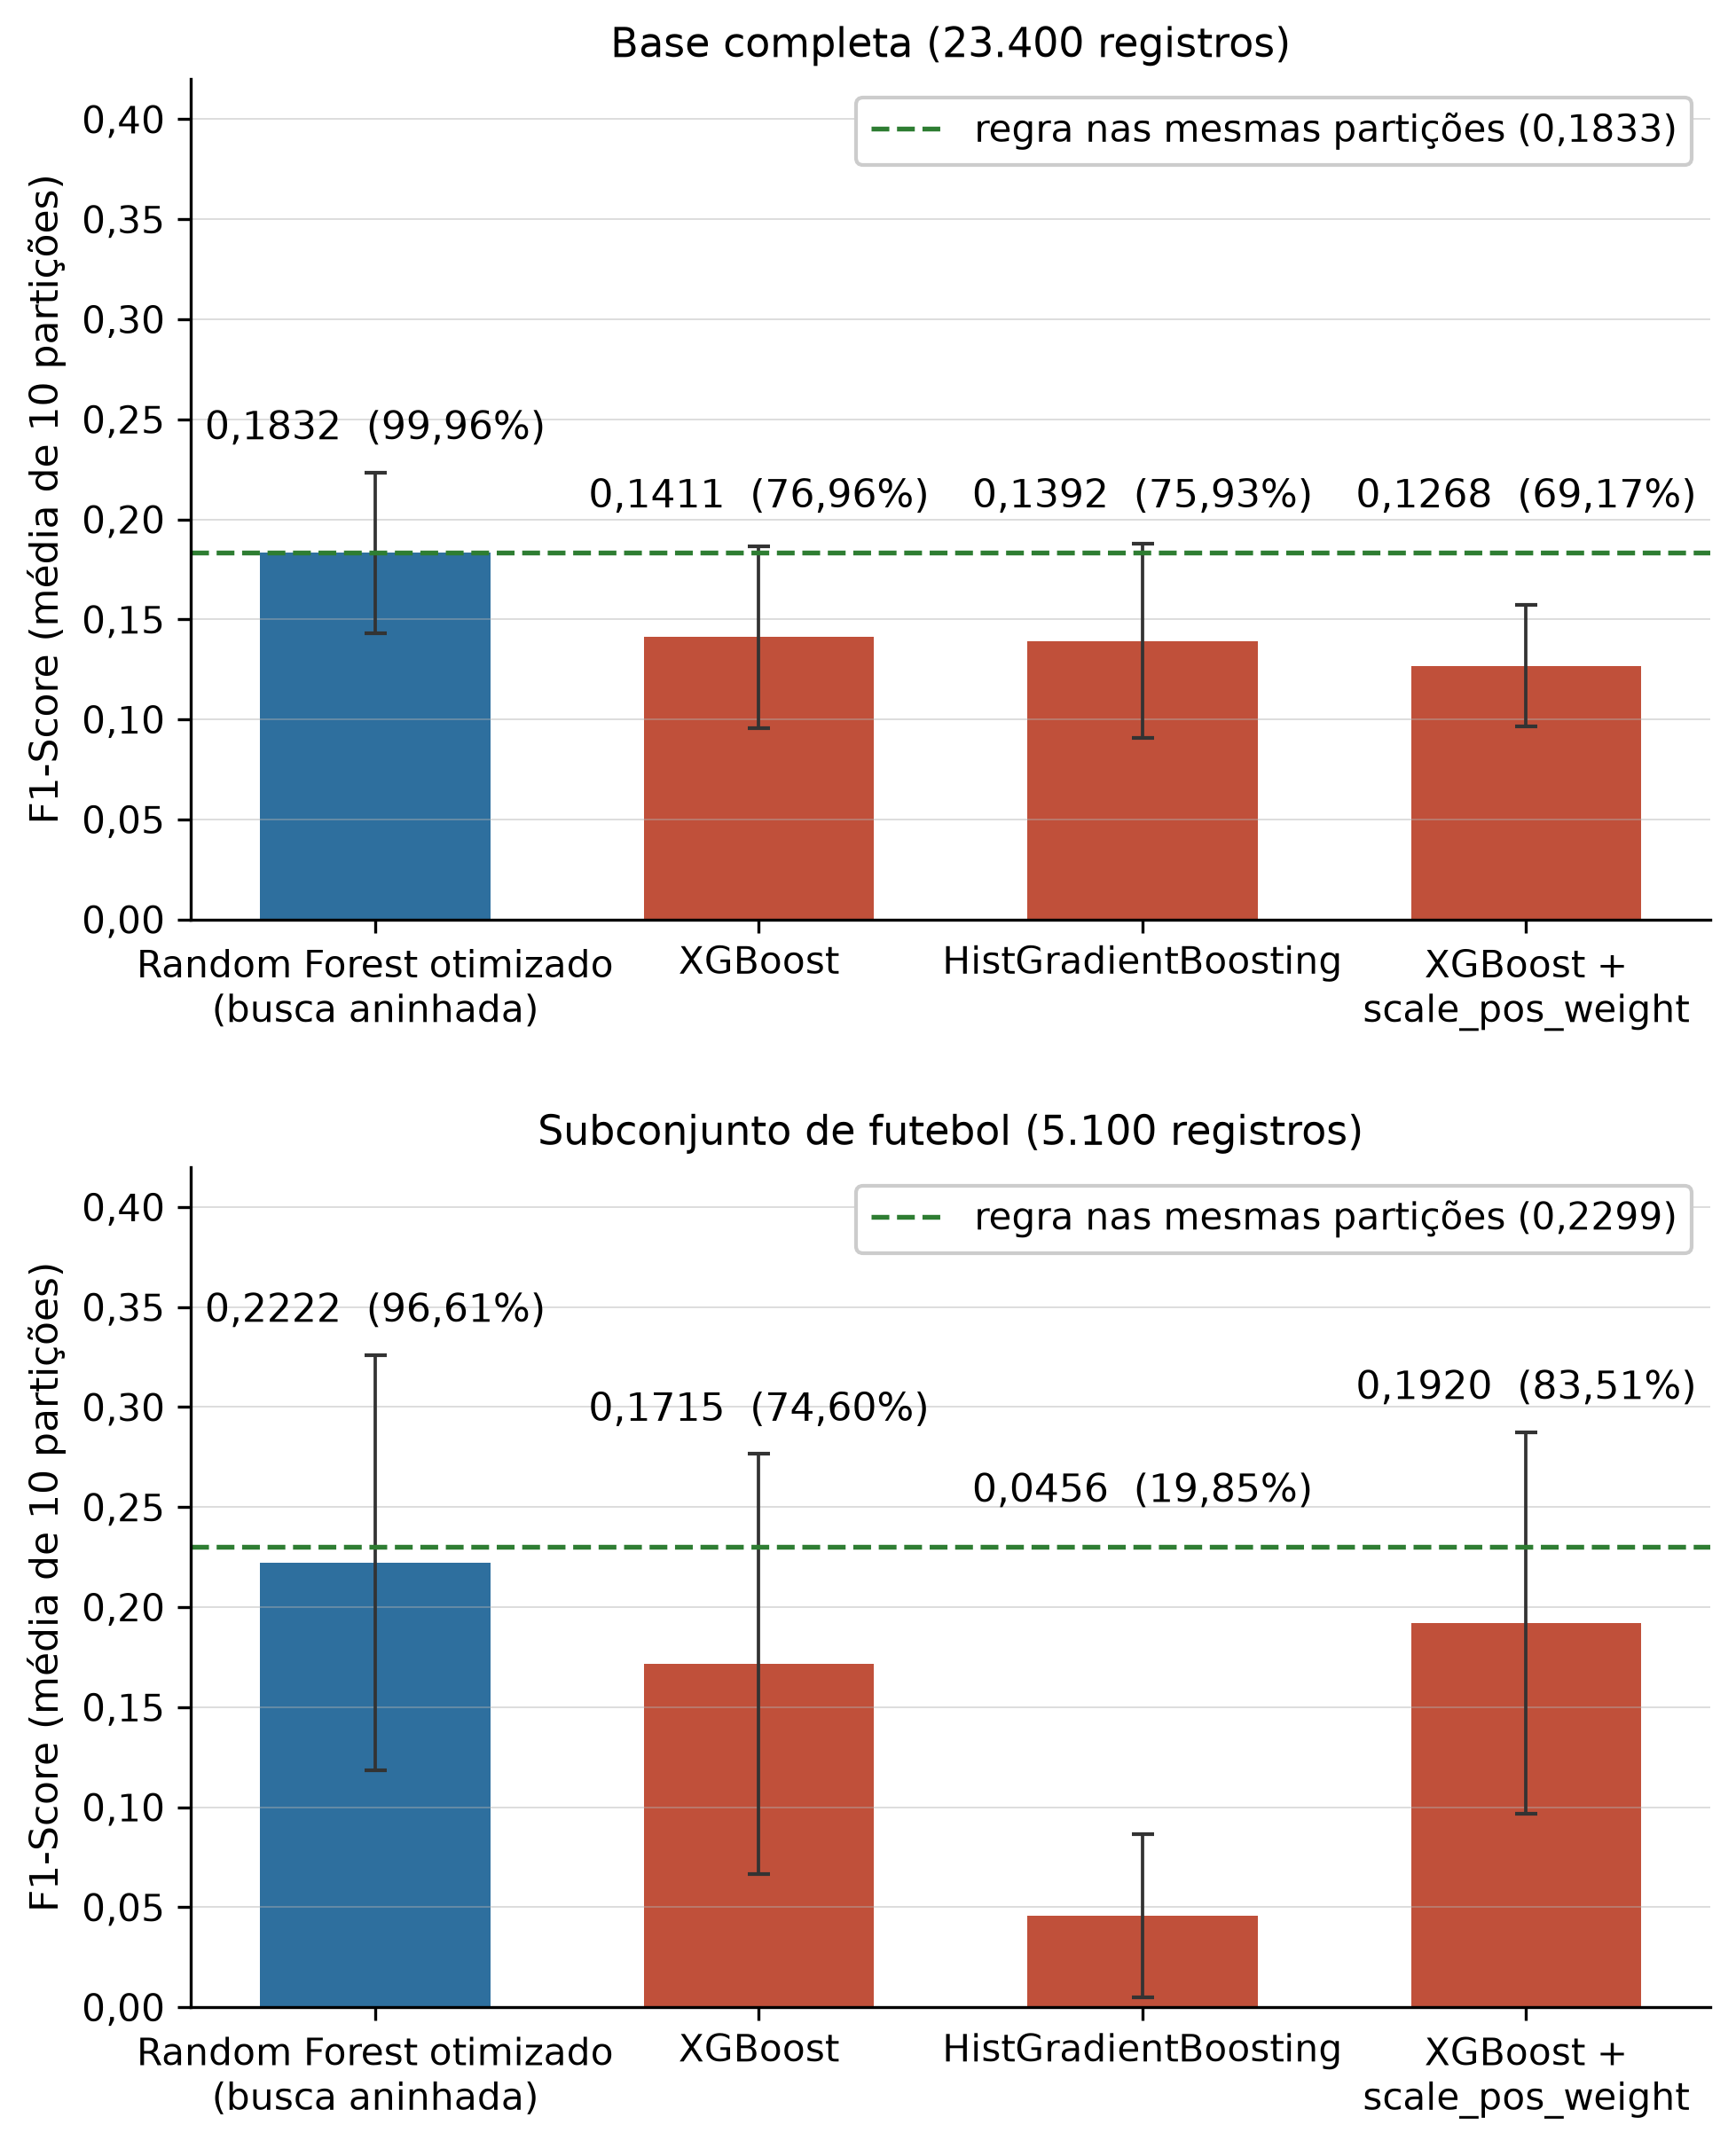
\includegraphics[width=\textwidth]{fig_leve/36_robustez_referencia_v4.png}
    \caption{Teste de robustez nos dois conjuntos de dados.}
    \label{fig:boosting}
\end{figure}

Na Figura~\ref{fig:boosting}, o painel superior corresponde à base completa e o inferior, ao subconjunto de futebol. As barras indicam o F1-Score médio de 10 \textit{folds} e as hastes, o desvio-padrão entre \textit{folds}, e a linha tracejada marca o F1-Score médio da regra nas mesmas partições, que nenhuma das configurações avaliadas supera.

Esses resultados são consistentes com a referência derivada na Seção~\ref{sec:limite} por duas vias. A primeira é que a busca de hiperparâmetros não produziu ganho algum. Na base completa, o \textit{Random Forest} otimizado sob busca aninhada alcançou F1 = $0{,}1832 \pm 0{,}0401$, praticamente igual ao da configuração \textit{baseline} reportada na Tabela~\ref{tab:resultados} (0{,}1833). No subconjunto de futebol, obteve 0{,}2222, valor igual ao do \textit{baseline}. Na busca conduzida uma única vez sobre a base completa, descrita na Seção~\ref{sec:busca}, a configuração selecionada foi \texttt{max\_depth = 5}, \texttt{class\_weight = None} e apenas 100 árvores. Essa observação deve ser lida com cuidado, pois o parâmetro \texttt{max\_depth} fixa a profundidade \textit{máxima permitida}, e não a profundidade efetivamente utilizada pelas árvores ajustadas. Além disso, a disjunção da Equação~\ref{eq:regra} pode ser representada por uma árvore de profundidade 2, de modo que o valor selecionado não corresponde à complexidade mínima necessária para codificá-la. O que o resultado permite afirmar é mais modesto: uma configuração de profundidade limitada e sem ponderação de classes alcançou desempenho equivalente ao da regra identificada, sem que o aumento de capacidade trouxesse ganho. No subconjunto de futebol, esse mesmo desenho não aninhado resultou em desempenho ligeiramente inferior ao \textit{baseline} (0{,}2130 contra 0{,}2222).

A segunda via é que os modelos de \textit{gradient boosting} apresentaram desempenho inferior ao \textit{Random Forest} em ambos os conjuntos, chegando a 69{,}17\% do F1-Score da regra na base completa e a 19{,}85\% no subconjunto de futebol. Esse resultado é observacional e comporta mais de uma explicação, que os experimentos conduzidos não permitem separar, entre as quais três fatores são plausíveis.

O primeiro fator é a razão sinal-ruído da base. Como a Seção~\ref{sec:residuo} indica, a parcela aprendível corresponde a 132 registros em 23.400, e o restante não apresentou sinal detectável. O \textit{boosting} opera por ajuste sequencial: cada estimador é treinado para corrigir os erros do anterior. Em um cenário no qual os erros remanescentes carecem de estrutura, iterações adicionais tendem a ajustar flutuação amostral. O \textit{Random Forest}, que agrega estimadores independentes por votação, está menos exposto a esse mecanismo. Trata-se de uma explicação compatível com os resultados, não de uma demonstração.

O segundo é a assimetria de esforço de ajuste apontada na Seção~\ref{sec:busca}. Apenas o \textit{Random Forest} passou por busca de hiperparâmetros, e parte da diferença pode decorrer disso.

O terceiro é o limiar de decisão: todas as métricas foram calculadas no limiar padrão de $0{,}5$, e algoritmos distintos produzem distribuições de probabilidade distintas. Uma calibração específica por algoritmo poderia alterar o ordenamento observado.

A tentativa de compensar o desbalanceamento agrava o problema. O XGBoost com \texttt{scale\_pos\_weight} teve a precisão reduzida de 0{,}8241 para 0{,}1332 na base completa, em troca de um aumento marginal de Recall (0{,}0775 para 0{,}1216), resultando no pior F1 \textit{entre as configurações de gradient boosting avaliadas nesta seção}. A Tabela~\ref{tab:resultados} contém configurações com F1 inferior a esse valor, de modo que a comparação não se estende ao experimento como um todo. A ponderação amplifica o peso de exemplos positivos que, em sua maioria, são indistinguíveis dos negativos.

Resta comparar a busca aninhada com o desenho não aninhado descrito na Seção~\ref{sec:busca}, que em princípio favorece a configuração selecionada. A Tabela~\ref{tab:aninhada} compara os dois desenhos na base completa, nas mesmas dez partições agrupadas por atleta, com média $\pm$ desvio-padrão entre partições.

\begin{table}[H]
\centering
\caption{Busca de hiperparâmetros não aninhada e aninhada.}
\label{tab:aninhada}
\resizebox{\textwidth}{!}{%
\begin{tabular}{lrrrr}
\toprule
Desenho da busca & Precisão & Recall & F1-Score & ROC-AUC \\
\midrule
Aninhada, independente por partição & $0{,}8980 \pm 0{,}2052$ & $0{,}1037 \pm 0{,}0249$ & $0{,}1832 \pm 0{,}0401$ & $0{,}5532 \pm 0{,}0300$ \\
Não aninhada, sobre a base completa & $1{,}0000 \pm 0{,}0000$ & $0{,}1014 \pm 0{,}0246$ & $0{,}1833 \pm 0{,}0401$ & $0{,}5604 \pm 0{,}0237$ \\
\bottomrule
\end{tabular}%
}
\end{table}

A diferença em F1-Score entre os dois desenhos é de $0{,}0001$, ordem de grandeza muito inferior ao desvio-padrão entre partições. Nesta base, portanto, o desenho não aninhado não inflou o valor relatado. No subconjunto de futebol, a busca aninhada obteve F1-Score de 0{,}2222, acima dos 0{,}2130 do desenho não aninhado, de modo que também ali o desenho não aninhado não favoreceu o resultado. Convém não generalizar essa constatação: o viés de seleção associado à busca não aninhada é real e pode ser expressivo quando existe sinal a explorar. A ausência de efeito aqui é coerente com a leitura proposta, uma vez que nenhuma configuração consegue extrair mais do que a regra já fornece.

Dois aspectos do resultado aninhado reforçam essa leitura. O primeiro é a instabilidade da configuração escolhida: ao longo das dez partições, a busca selecionou três valores distintos para o número de árvores, quatro para o mínimo de amostras por divisão, três para a profundidade máxima e dois para a ponderação de classes. Não há convergência para uma configuração preferida, comportamento esperado quando as diferenças de desempenho entre configurações são indistinguíveis da variação amostral. O segundo é que a precisão permaneceu exatamente $1{,}0000$ em oito das dez partições, caindo para $0{,}5385$ e $0{,}4412$ nas duas restantes. Nessas duas a busca havia selecionado \texttt{class\_weight = balanced}, embora a mesma opção tenha sido escolhida em outras três partições sem que a precisão se alterasse, de modo que o desenho adotado não permite atribuir a queda a esse parâmetro isoladamente.

Em conjunto, os dois experimentos reforçam a leitura proposta sem, contudo, demonstrá-la: nenhuma das configurações avaliadas superou a regra aplicada às mesmas partições ($0{,}1833$ na base completa e $0{,}2299$ no subconjunto de futebol), e várias ficaram substancialmente abaixo dela. Esse resultado mostra que, no conjunto de algoritmos e configurações testados, o aumento de capacidade não produziu ganho, mas não demonstra que nenhum outro modelo poderia superar a referência, afirmação que exigiria um espaço de busca exaustivo, inviável na prática.

\subsection{Ajuste do Limiar de Decisão}

O ajuste de limiar foi conduzido sobre as três partições disjuntas descritas na Seção~\ref{sec:estrategias}: treinamento com 140 atletas e 14.000 registros, calibração com 47 atletas e 4.700 registros, e avaliação com 47 atletas e 4.700 registros. A verificação de sobreposição confirmou que nenhum atleta aparece em mais de uma partição. Como essas partições são fixas, e não obtidas por validação cruzada, os resultados não são diretamente comparáveis aos das 11 configurações da Tabela~\ref{tab:resultados}.

A Figura~\ref{fig:pr_curve} apresenta a curva Precisão $\times$ Recall e o comportamento das métricas em função do limiar, calculados sobre a partição de calibração, que é onde a escolha ocorre. O limiar que maximiza o F1-Score nessa partição é $0{,}4750$.

\begin{figure}[H]
    \centering
    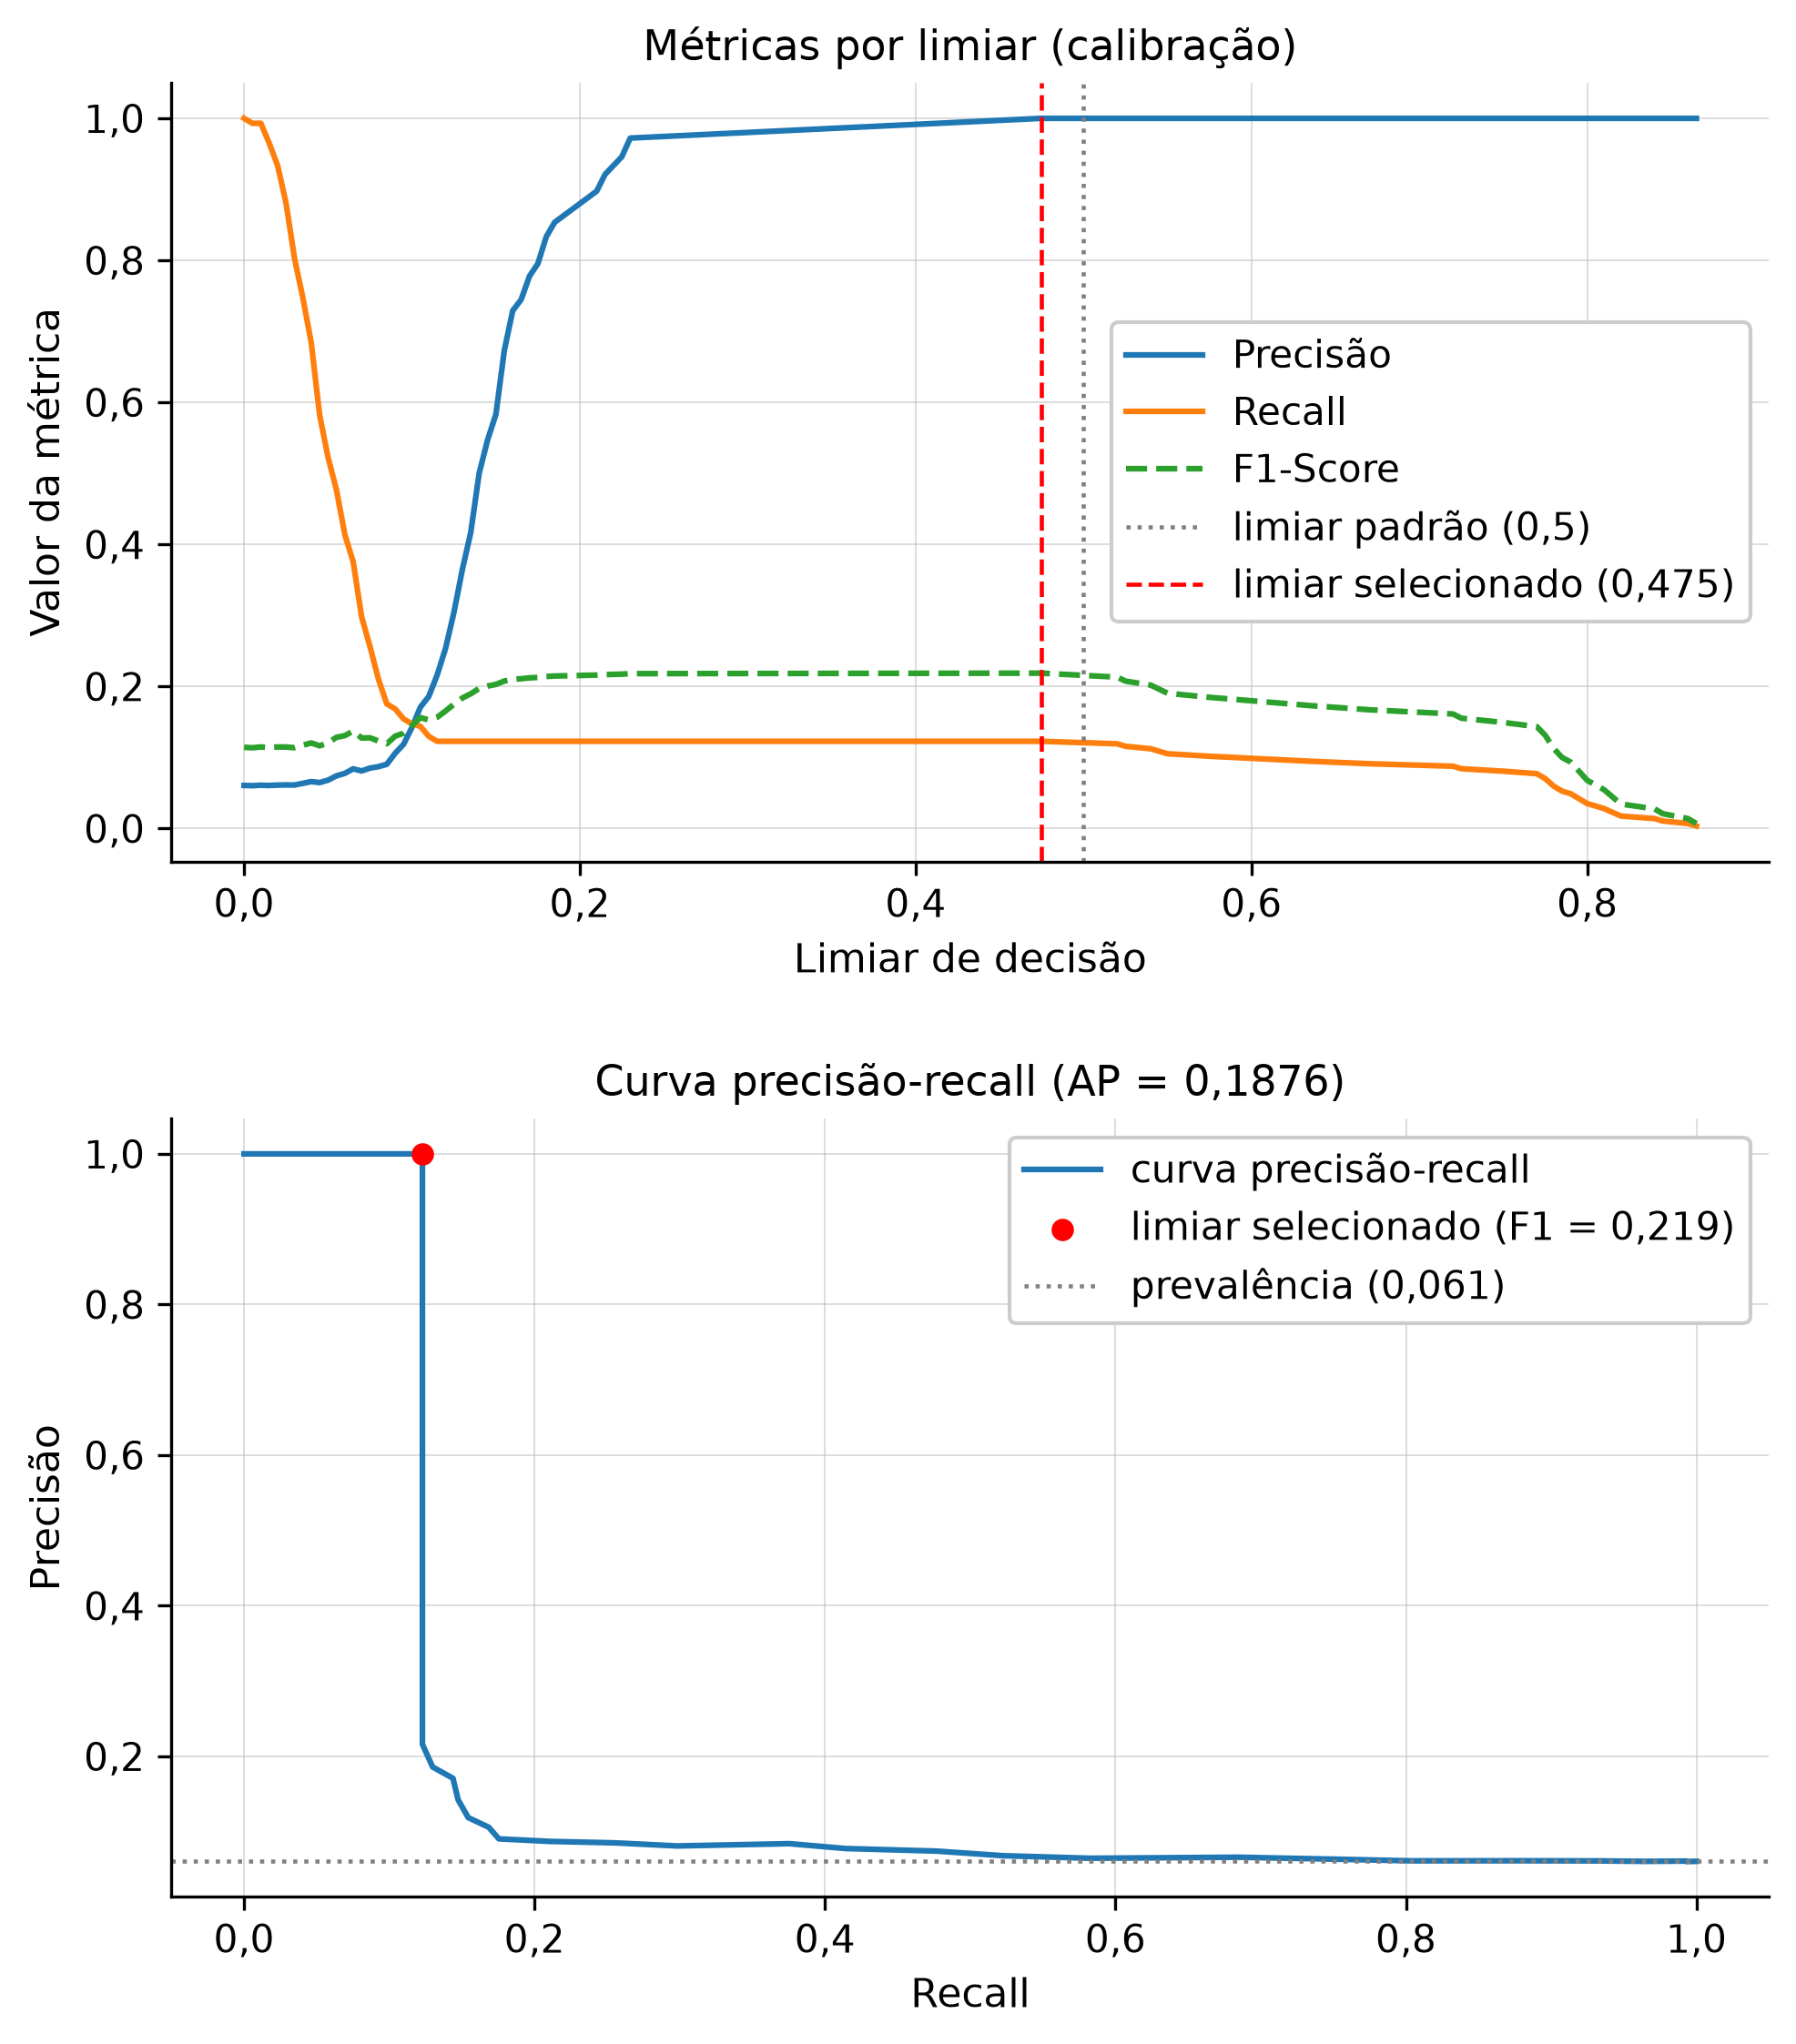
\includegraphics[width=\textwidth]{fig_leve/39_curva_limiar_calibracao_v3.png}
    \caption{Métricas por limiar e curva precisão-recall.}
    \label{fig:pr_curve}
\end{figure}

Os dois painéis da figura foram calculados na partição de calibração, e AP indica a precisão média. Aplicado à partição de avaliação, que não participou nem do ajuste do modelo nem da escolha do limiar, o limiar selecionado produz o resultado da Tabela~\ref{tab:limiar}, que o compara ao limiar padrão. As duas linhas diferem apenas no recall e, por consequência, no F1-Score.

\begin{table}[H]
\centering
\caption{Desempenho na partição de avaliação sob os dois limiares.}
\label{tab:limiar}
\begin{tabular}{lrrr}
\toprule
Limiar & Precisão & Recall & F1-Score \\
\midrule
Padrão ($0{,}5000$)       & 1{,}0000 & 0{,}0913 & 0{,}1673 \\
Calibrado ($0{,}4750$)    & 1{,}0000 & 0{,}0954 & 0{,}1742 \\
\bottomrule
\end{tabular}
\end{table}

O ganho é de $0{,}0069$ em F1-Score, e decorre da reclassificação de um único registro entre os 4.700 avaliados. A razão está na distribuição das probabilidades atribuídas pelo modelo: 4.395 dos 4.700 registros receberam probabilidade inferior a $0{,}100$, e apenas 22 ficaram acima de $0{,}500$. Entre o limiar calibrado e o padrão havia um único registro, com probabilidade $0{,}480$. As estimativas são fortemente polarizadas, e a faixa intermediária, onde o deslocamento do limiar produziria efeito, está praticamente vazia. Esse comportamento explica a Figura~\ref{fig:confusao}, que contrasta as matrizes de confusão sob os dois limiares.

\begin{figure}[H]
    \centering
    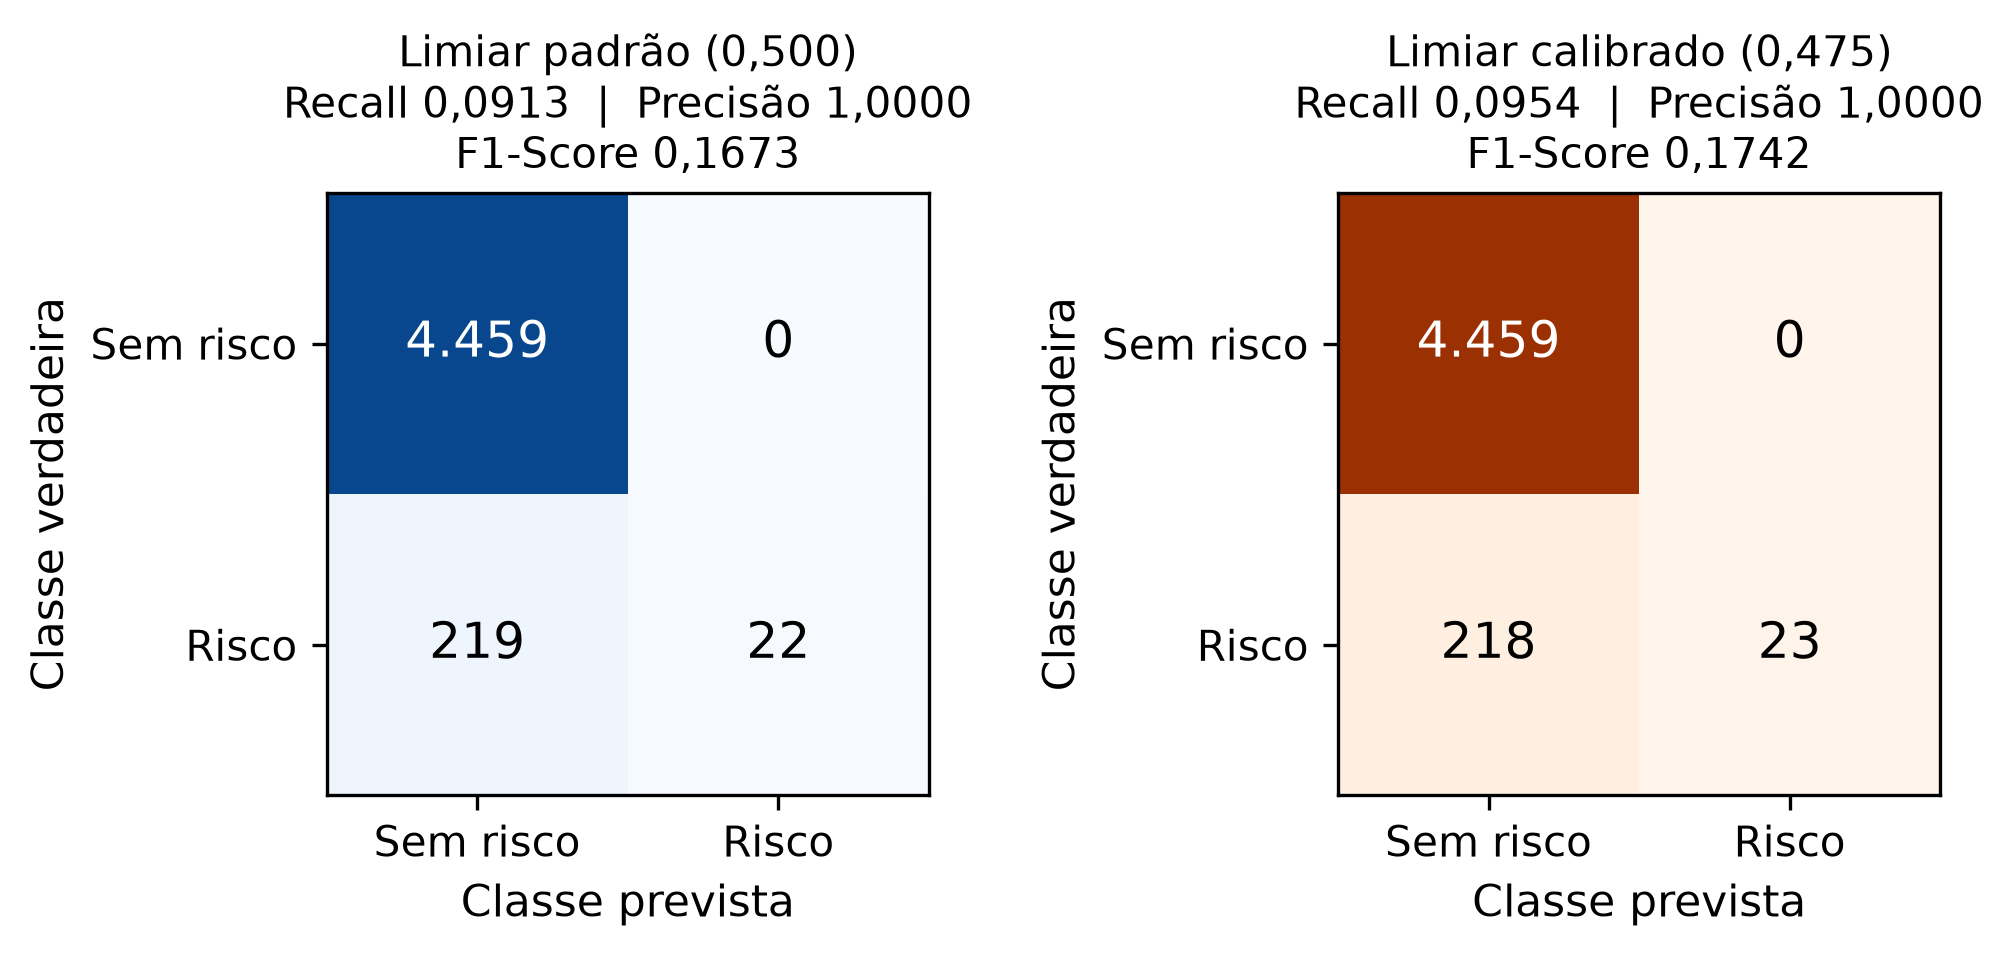
\includegraphics[width=\textwidth]{fig_leve/40_matrizes_confusao_avaliacao_v3.png}
    \caption{Matrizes de confusão nos dois limiares.}
    \label{fig:confusao}
\end{figure}

A matriz da esquerda corresponde ao limiar padrão, de 0{,}5, e a da direita, ao limiar calibrado. A diferença entre as duas se resume a um único registro, que deixa de ser falso negativo e passa a verdadeiro positivo, o que confirma a concentração das probabilidades estimadas nos extremos.

Na literatura, a calibração de limiar é apresentada como recurso para deslocar o equilíbrio entre precisão e recall em cenários de classe rara. Nesta base, esse recurso teve efeito praticamente nulo, e o motivo é informativo: quando o modelo atribui probabilidades concentradas nos extremos, não existe faixa intermediária sobre a qual o limiar possa operar. A ausência de ganho, portanto, não indica falha do procedimento, e sim que a estrutura das estimativas não oferece margem para esse tipo de ajuste.

\section{Explicabilidade}

Esta seção examina em quais variáveis os classificadores se apoiam, por meio das três técnicas de explicabilidade e de uma árvore de decisão interpretável. O objetivo é verificar se essas variáveis correspondem às que compõem a regra identificada.

\subsection{Convergência dos Três Métodos}
A Tabela~\ref{tab:ranking_xai} compara os \textit{rankings} de importância produzidos por Gini, Permutação e SHAP. Para cada método, as variáveis foram ordenadas da mais para a menos importante, e a tabela mostra a posição ocupada por cada uma. Estão incluídas as duas variáveis da regra e as três de maior divergência entre os métodos.

\begin{table}[H]
\centering
\caption{\textit{Ranking} de importância das variáveis por três métodos.}
\label{tab:ranking_xai}
\begin{tabular}{lccc}
\toprule
Variável & Gini & Permutação & SHAP \\
\midrule
Heart\_Rate              & 1\textordmasculine & 1\textordmasculine & 1\textordmasculine \\
Muscle\_Activity          & 2\textordmasculine & 2\textordmasculine & 2\textordmasculine \\
Oxygen\_Saturation        & 4\textordmasculine & 4\textordmasculine & 3\textordmasculine \\
Motion\_Z                 & 3\textordmasculine & 14\textordmasculine & 4\textordmasculine \\
Age                       & 7\textordmasculine & 3\textordmasculine & 7\textordmasculine \\
\bottomrule
\end{tabular}
\end{table}

Os três métodos coincidem nas duas primeiras posições, \texttt{Heart\_Rate} e \texttt{Muscle\_Activity}, que são as variáveis presentes na regra da Equação~\ref{eq:regra}. A partir da terceira posição os ordenamentos divergem de forma substancial: a Importância por Permutação posiciona \texttt{Motion\_Z} em décimo quarto lugar, enquanto Gini a coloca em terceiro, e \texttt{Age}, sétima para Gini e SHAP, é terceira para a Permutação. Essa divergência é esperada em uma região onde não há sinal a ordenar, e cada método ordena flutuação segundo seus próprios critérios.

Cabe delimitar o que essa coincidência permite afirmar. Ela indica que os critérios internos do modelo ajustado são consistentes com a regra identificada na Seção~\ref{sec:regra}, o que é um teste de coerência entre duas análises conduzidas sobre os mesmos dados. Não constitui validação independente do procedimento que gerou os rótulos, já que tanto a regra quanto o modelo foram obtidos a partir da mesma amostra. Tampouco constitui evidência de relação fisiológica entre as variáveis e o desfecho: a associação observada é artefato do procedimento de geração da base, e não achado sobre atletas.

No caso do SHAP, a coincidência nas duas primeiras posições exige uma ressalva adicional, discutida na Seção~\ref{sec:shap}. As condições de cálculo dos três métodos, incluindo o modelo sobre o qual foram aplicados e o tamanho das amostras utilizadas, constam da Seção~\ref{sec:reprodutibilidade}.

\subsection{Árvore de Decisão Interpretável}
A Figura~\ref{fig:arvore} apresenta a árvore de decisão ilustrativa descrita na Seção~\ref{sec:explic_metodo}, cujos limiares aparecem nas unidades originais das variáveis. Ela serve apenas para visualizar os cortes, e não integra a comparação de desempenho.

\begin{figure}[H]
    \centering
    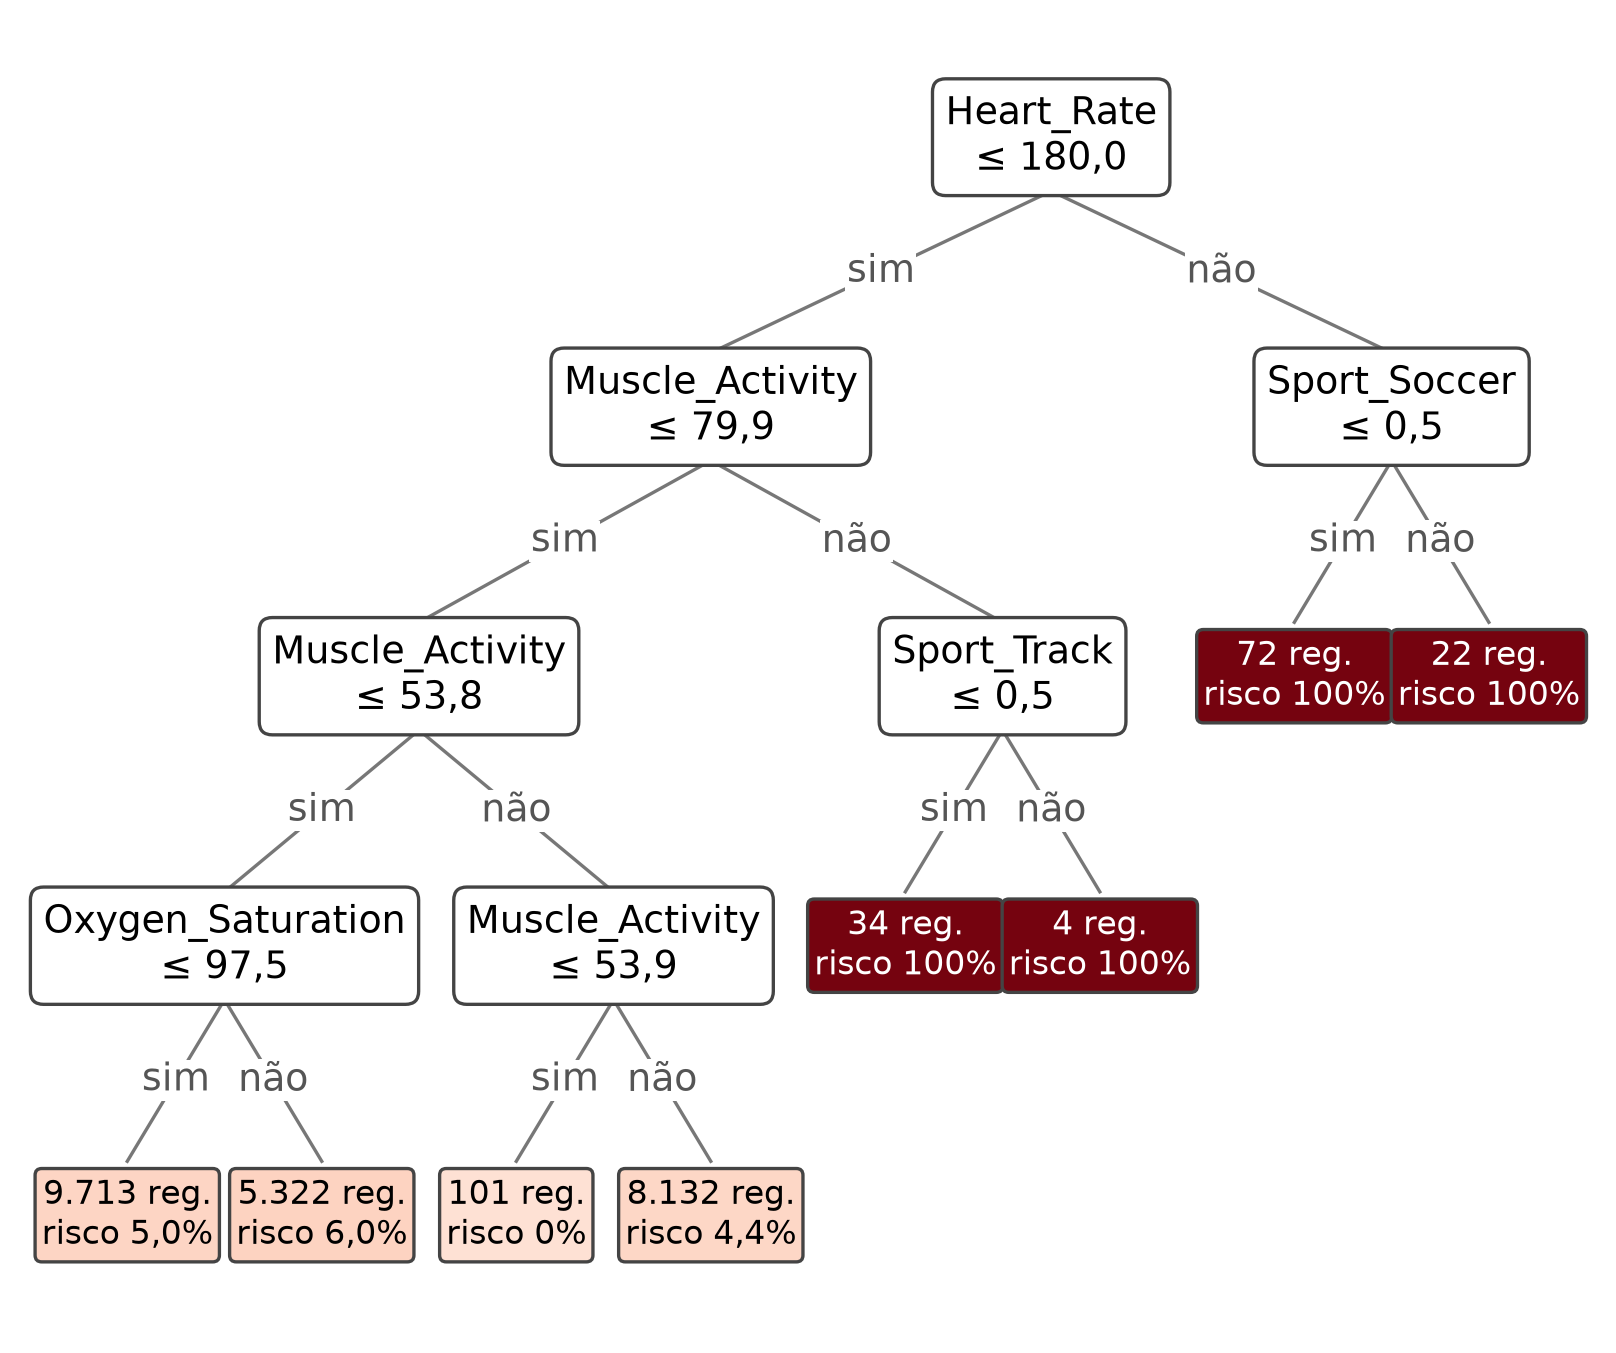
\includegraphics[width=\textwidth]{fig_leve/30_arvore_decisao_legivel_v3.png}
    \caption{Árvore de Decisão ilustrativa, em unidades originais.}
    \label{fig:arvore}
\end{figure}

Cada nó interno da figura mostra o teste aplicado, e cada folha, o número de registros que reúne e a taxa observada de risco entre eles, que também determina a cor. O nó raiz corresponde a um dos dois testes que compõem a Equação~\ref{eq:regra}, $\texttt{Heart\_Rate} \leq 180$ bpm, e não à disjunção completa. O segundo teste, sobre \texttt{Muscle\_Activity}, aparece no nível seguinte.

As quatro folhas situadas além desses dois testes, com \texttt{Heart\_Rate} acima de 180 ou \texttt{Muscle\_Activity} acima de 79{,}9, somam 132 registros, todos positivos, que são exatamente os registros abrangidos pela regra. As divisões adicionais, por modalidade esportiva, apenas repartem esse conjunto. Do outro lado, as divisões abaixo do segundo nível separam grupos com taxas de risco entre 4{,}4\% e 6{,}0\%, próximas da taxa do resíduo. A exceção é uma folha de 101 registros sem nenhum positivo, definida por uma faixa estreita de \texttt{Muscle\_Activity}, entre 53{,}8 e 53{,}9. Trata-se de um efeito de seleção: entre os muitos cortes possíveis, a árvore escolhe aquele que, por acaso, isola um grupo pequeno sem positivos.

\subsection{SHAP: Contribuição Individual das Variáveis}
\label{sec:shap}

Enquanto a Importância de Gini e a Importância por Permutação produzem um valor agregado por variável, os valores SHAP quantificam a contribuição de cada variável em cada predição individual. A Figura~\ref{fig:shap_beeswarm} apresenta essa distribuição, e a Figura~\ref{fig:shap_bar} a consolida em importância média absoluta por variável.

A leitura dessas figuras exige uma observação sobre a amostra. A subamostra de 800 registros, sorteada da partição de avaliação, contém um único registro na região da regra, com \texttt{Heart\_Rate} acima de 180, e nenhum com \texttt{Muscle\_Activity} acima de 80. É nesse registro que aparece a única contribuição positiva expressiva, de $0{,}56$, atribuída a \texttt{Heart\_Rate}. Nos 799 registros restantes, as contribuições de \texttt{Heart\_Rate} e de \texttt{Muscle\_Activity} são negativas independentemente do valor da variável: mesmo entre os 10\% de maior valor fora da regra, a contribuição média é de aproximadamente $-0{,}07$ para ambas. O modelo, portanto, não trata valores elevados dessas variáveis como indício geral de risco; reage apenas à região delimitada pela regra.

O sinal negativo generalizado tem origem na ponderação de classes. Com \texttt{class\_weight = balanced}, o valor esperado da saída do modelo é de $0{,}4991$, enquanto a maioria dos registros recebe probabilidade próxima de zero. Pela propriedade aditiva do método, as contribuições de cada registro somam a diferença entre sua probabilidade estimada e esse valor esperado, e essa diferença é repartida entre as variáveis. A importância média absoluta mede, por isso, sobretudo a forma como o modelo reparte essa redução, e não sua capacidade de reconhecer risco. As diferenças entre variáveis nessa medida são moderadas: $0{,}0808$ para \texttt{Heart\_Rate}, $0{,}0661$ para \texttt{Muscle\_Activity} e valores entre $0{,}0559$ e $0{,}0573$ para \texttt{Oxygen\_Saturation} e as três componentes de movimento.

A coincidência do SHAP com os demais métodos nas duas primeiras posições deve ser lida com essa ressalva, e é a parte de menor peso da convergência relatada. Há ainda uma diferença de modelo: os valores SHAP foram calculados sobre o \textit{Random Forest} com ponderação de classes descrito na Seção~\ref{sec:reprodutibilidade}, e não sobre o \textit{Random Forest} sem ponderação que reproduziu a regra registro a registro. Por essas razões, o resultado do SHAP tem caráter exploratório. Uma subamostra estratificada, que incluísse os 26 registros da regra presentes na partição de avaliação, permitiria examinar a contribuição das variáveis nessa região com mais exemplos, e fica registrada como limitação desta análise.

\begin{figure}[H]
    \centering
    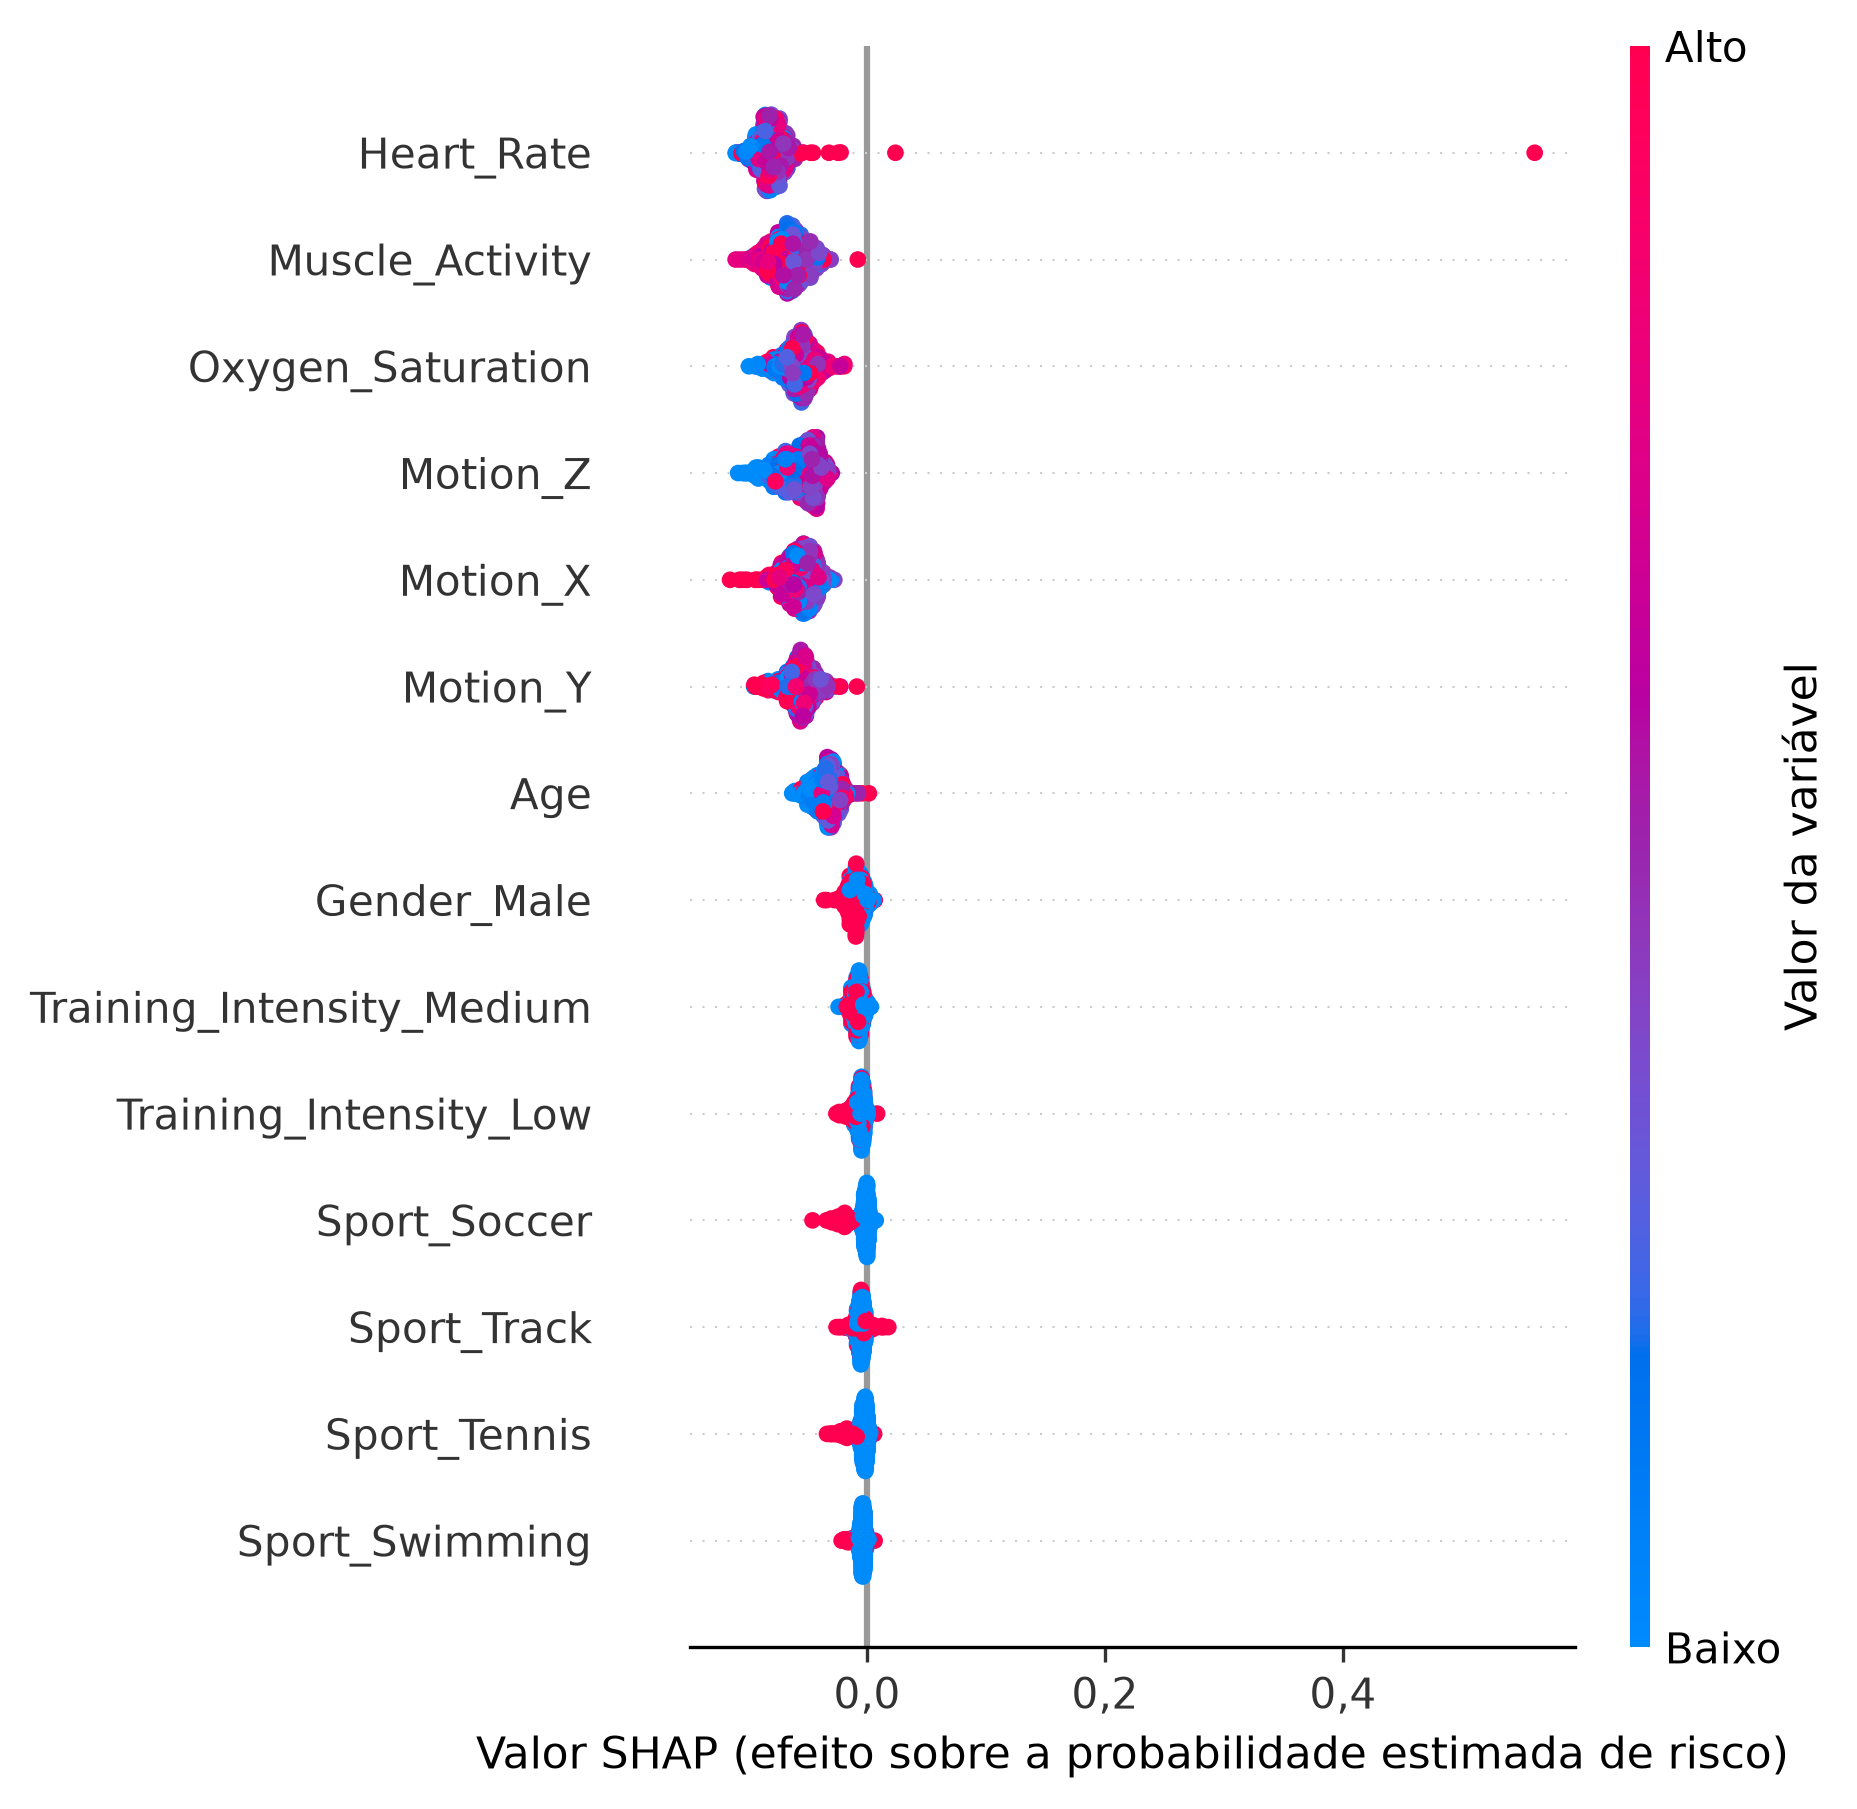
\includegraphics[width=\textwidth]{fig_leve/32_shap_beeswarm_v3.png}
    \caption{SHAP \textit{beeswarm}: contribuição por registro.}
    \label{fig:shap_beeswarm}
\end{figure}

Cada ponto da figura é um dos 800 registros da subamostra, e a cor indica o valor da variável naquele registro, em vermelho para valores altos e em azul para valores baixos. O ponto isolado à direita na linha de \texttt{Heart\_Rate} é o único registro da subamostra situado na região da regra. A Figura~\ref{fig:shap_bar} resume essas contribuições pela média do valor absoluto de cada variável.

\begin{figure}[H]
    \centering
    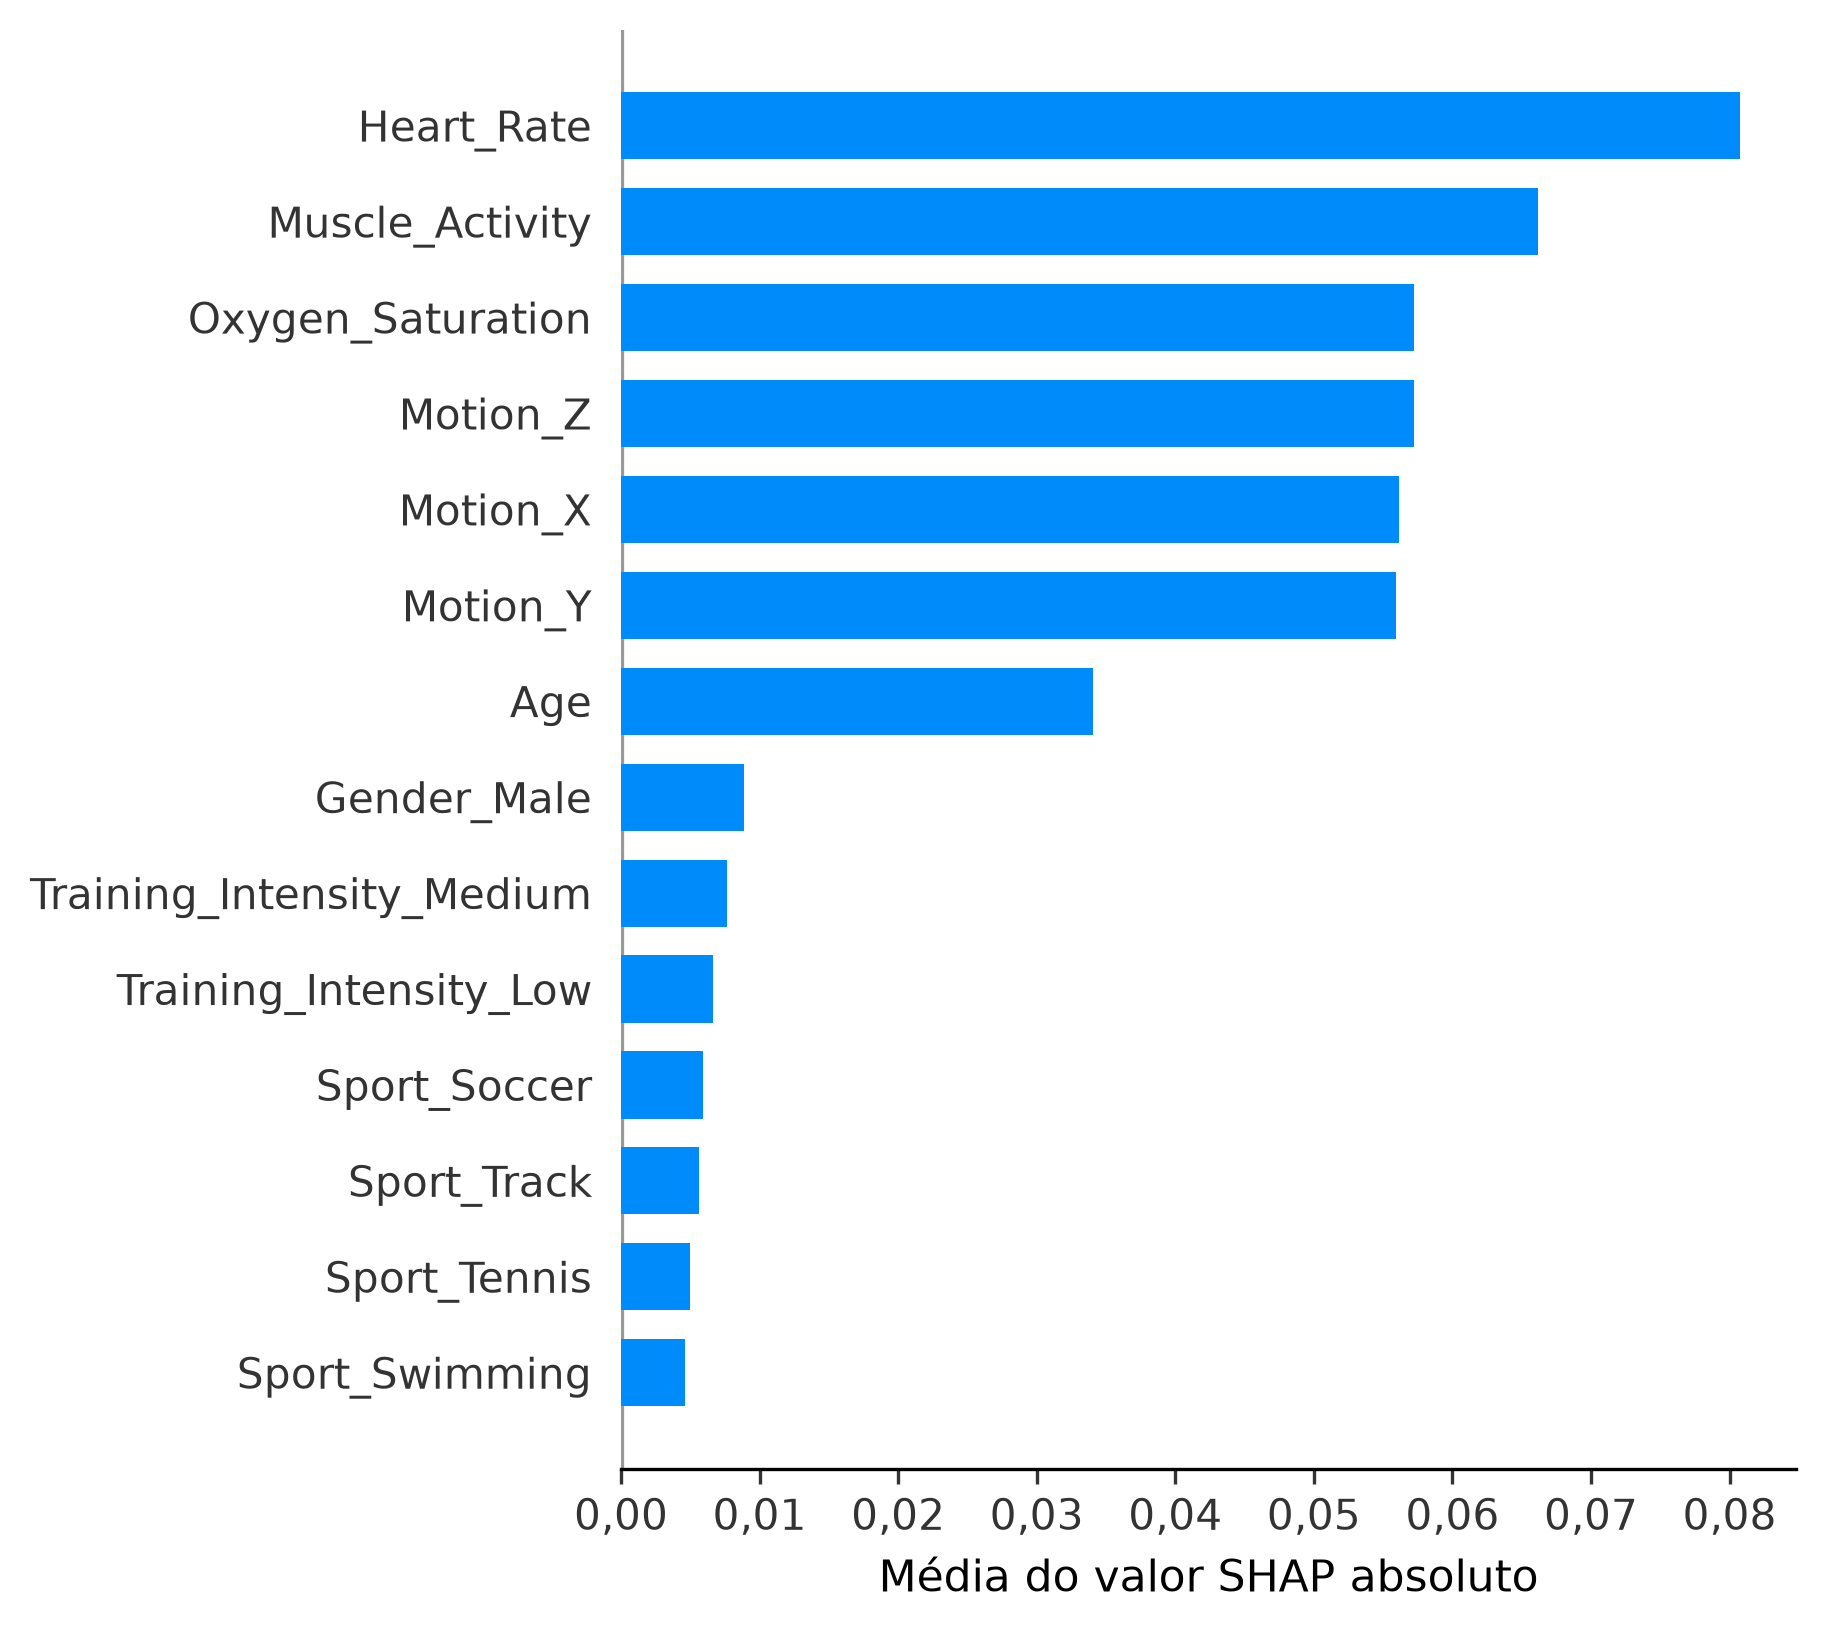
\includegraphics[width=\textwidth]{fig_leve/33_shap_bar_v3.png}
    \caption{SHAP: importância média absoluta por variável.}
    \label{fig:shap_bar}
\end{figure}

\section{Comparação entre Protocolos de Avaliação}

Esta seção examina o efeito de dois erros de protocolo sobre as métricas relatadas: a geração de exemplos sintéticos antes da divisão dos dados e a sobreposição de registros de um mesmo atleta entre treino e teste. Em ambos os casos, o desempenho sob o protocolo inadequado é comparado ao obtido sob o protocolo adotado no restante do experimento.

\subsection{Reamostragem Antes da Divisão dos Dados}
\label{sec:smote_leak}
Esta subseção compara o \textit{Random Forest} sob dois protocolos. No primeiro, o SMOTE é aplicado ao conjunto completo antes de qualquer divisão. No segundo, é aplicado apenas à porção de treinamento de cada partição, por meio de \texttt{imblearn.pipeline.Pipeline}. A Tabela~\ref{tab:protocolos_smote} descreve as duas configurações em detalhe, porque a diferença entre elas não se resume ao momento de aplicação do SMOTE. Os valores de treino e teste da tabela referem-se a uma partição.

\begin{table}[H]
\centering
\caption{Caracterização dos dois protocolos de SMOTE.}
\label{tab:protocolos_smote}
\resizebox{\textwidth}{!}{%
\begin{tabular}{lrr}
\toprule
Característica & Protocolo A (inadequado) & Protocolo B (adequado) \\
\midrule
Registros disponíveis               & 44.206 & 23.400 \\
Registros sintéticos no conjunto    & 20.806 & 0 \\
Proporção de positivos no conjunto  & 0{,}5000 & 0{,}0554 \\
Registros de treino por partição    & 39.785 & 21.000 \\
Registros de teste por partição     & 4.421 & 2.400 \\
Proporção de positivos no teste     & 0{,}4999 & 0{,}0546 \\
Sintéticos dentro do teste          & 2.077 (47{,}0\%) & 0 \\
Método de divisão                   & \texttt{StratifiedKFold} & \texttt{StratifiedGroupKFold} \\
Agrupamento por atleta              & ausente & por \texttt{Athlete\_ID} \\
Atletas presentes em treino e teste & 234 de 234 & 0 de 234 \\
\bottomrule
\end{tabular}%
}
\end{table}

Três diferenças separam os protocolos, e elas atuam simultaneamente. A primeira é a presença de registros sintéticos no conjunto de avaliação: no protocolo A, 47\% das observações de teste são interpolações geradas a partir de registros que, em parte, estão no treinamento. A segunda é a composição do conjunto de avaliação, cuja proporção de positivos passa de 5{,}46\% para 49{,}99\%, alterando a própria base de comparação das métricas. A terceira é a ausência de agrupamento: no protocolo A, os 234 atletas aparecem simultaneamente em treino e teste.

Quanto ao tratamento das variáveis, o identificador \texttt{Athlete\_ID} foi removido da matriz de atributos antes da geração sintética, e portanto não participou da interpolação. As variáveis categóricas, por outro lado, foram submetidas a codificação \textit{one-hot} previamente, de modo que o SMOTE interpolou linearmente colunas binárias. O resultado são registros sintéticos com valores fracionários em atributos que admitem apenas 0 ou 1: entre 25{,}9\% e 49{,}5\% dos registros gerados apresentam valores intermediários nessas colunas, a depender do atributo. Trata-se de uma limitação conhecida da aplicação de SMOTE a dados mistos, e que não foi tratada neste experimento.

A Tabela~\ref{tab:leakage_smote} apresenta o desempenho do \textit{Random Forest} sob cada um dos dois protocolos completos. A última linha registra a diferença entre eles nas duas métricas em que ela é mais acentuada, o recall e a ROC-AUC.

\begin{table}[H]
\centering
\caption{Desempenho sob os dois protocolos de SMOTE.}
\label{tab:leakage_smote}
\begin{tabular}{lrrrrrr}
\toprule
Protocolo & Acurácia & Precisão & Recall & F1 & ROC-AUC & AP \\
\midrule
Protocolo A (inadequado) & 0{,}9727 & 0{,}9995 & 0{,}9459 & 0{,}9719 & 0{,}9865 & 0{,}9907 \\
Protocolo B (adequado)   & 0{,}9313 & 0{,}2492 & 0{,}1144 & 0{,}1549 & 0{,}5497 & 0{,}1504 \\
\addlinespace
Diferença (A $-$ B)      &          &          & +0{,}8315 &         & +0{,}4368 &         \\
\bottomrule
\end{tabular}
\end{table}

A diferença é expressiva: o Recall passa de 0{,}1144 para 0{,}9459 ($+0{,}8315$), e o ROC-AUC de 0{,}5497 para 0{,}9865 ($+0{,}4368$). Um experimento conduzido sob o protocolo A reportaria desempenho quase perfeito sobre uma base cuja parcela majoritária não apresentou sinal preditivo detectável, conforme a Seção~\ref{sec:residuo}. A Figura~\ref{fig:leakage} representa graficamente a magnitude dessa distorção.

\begin{figure}[H]
    \centering
    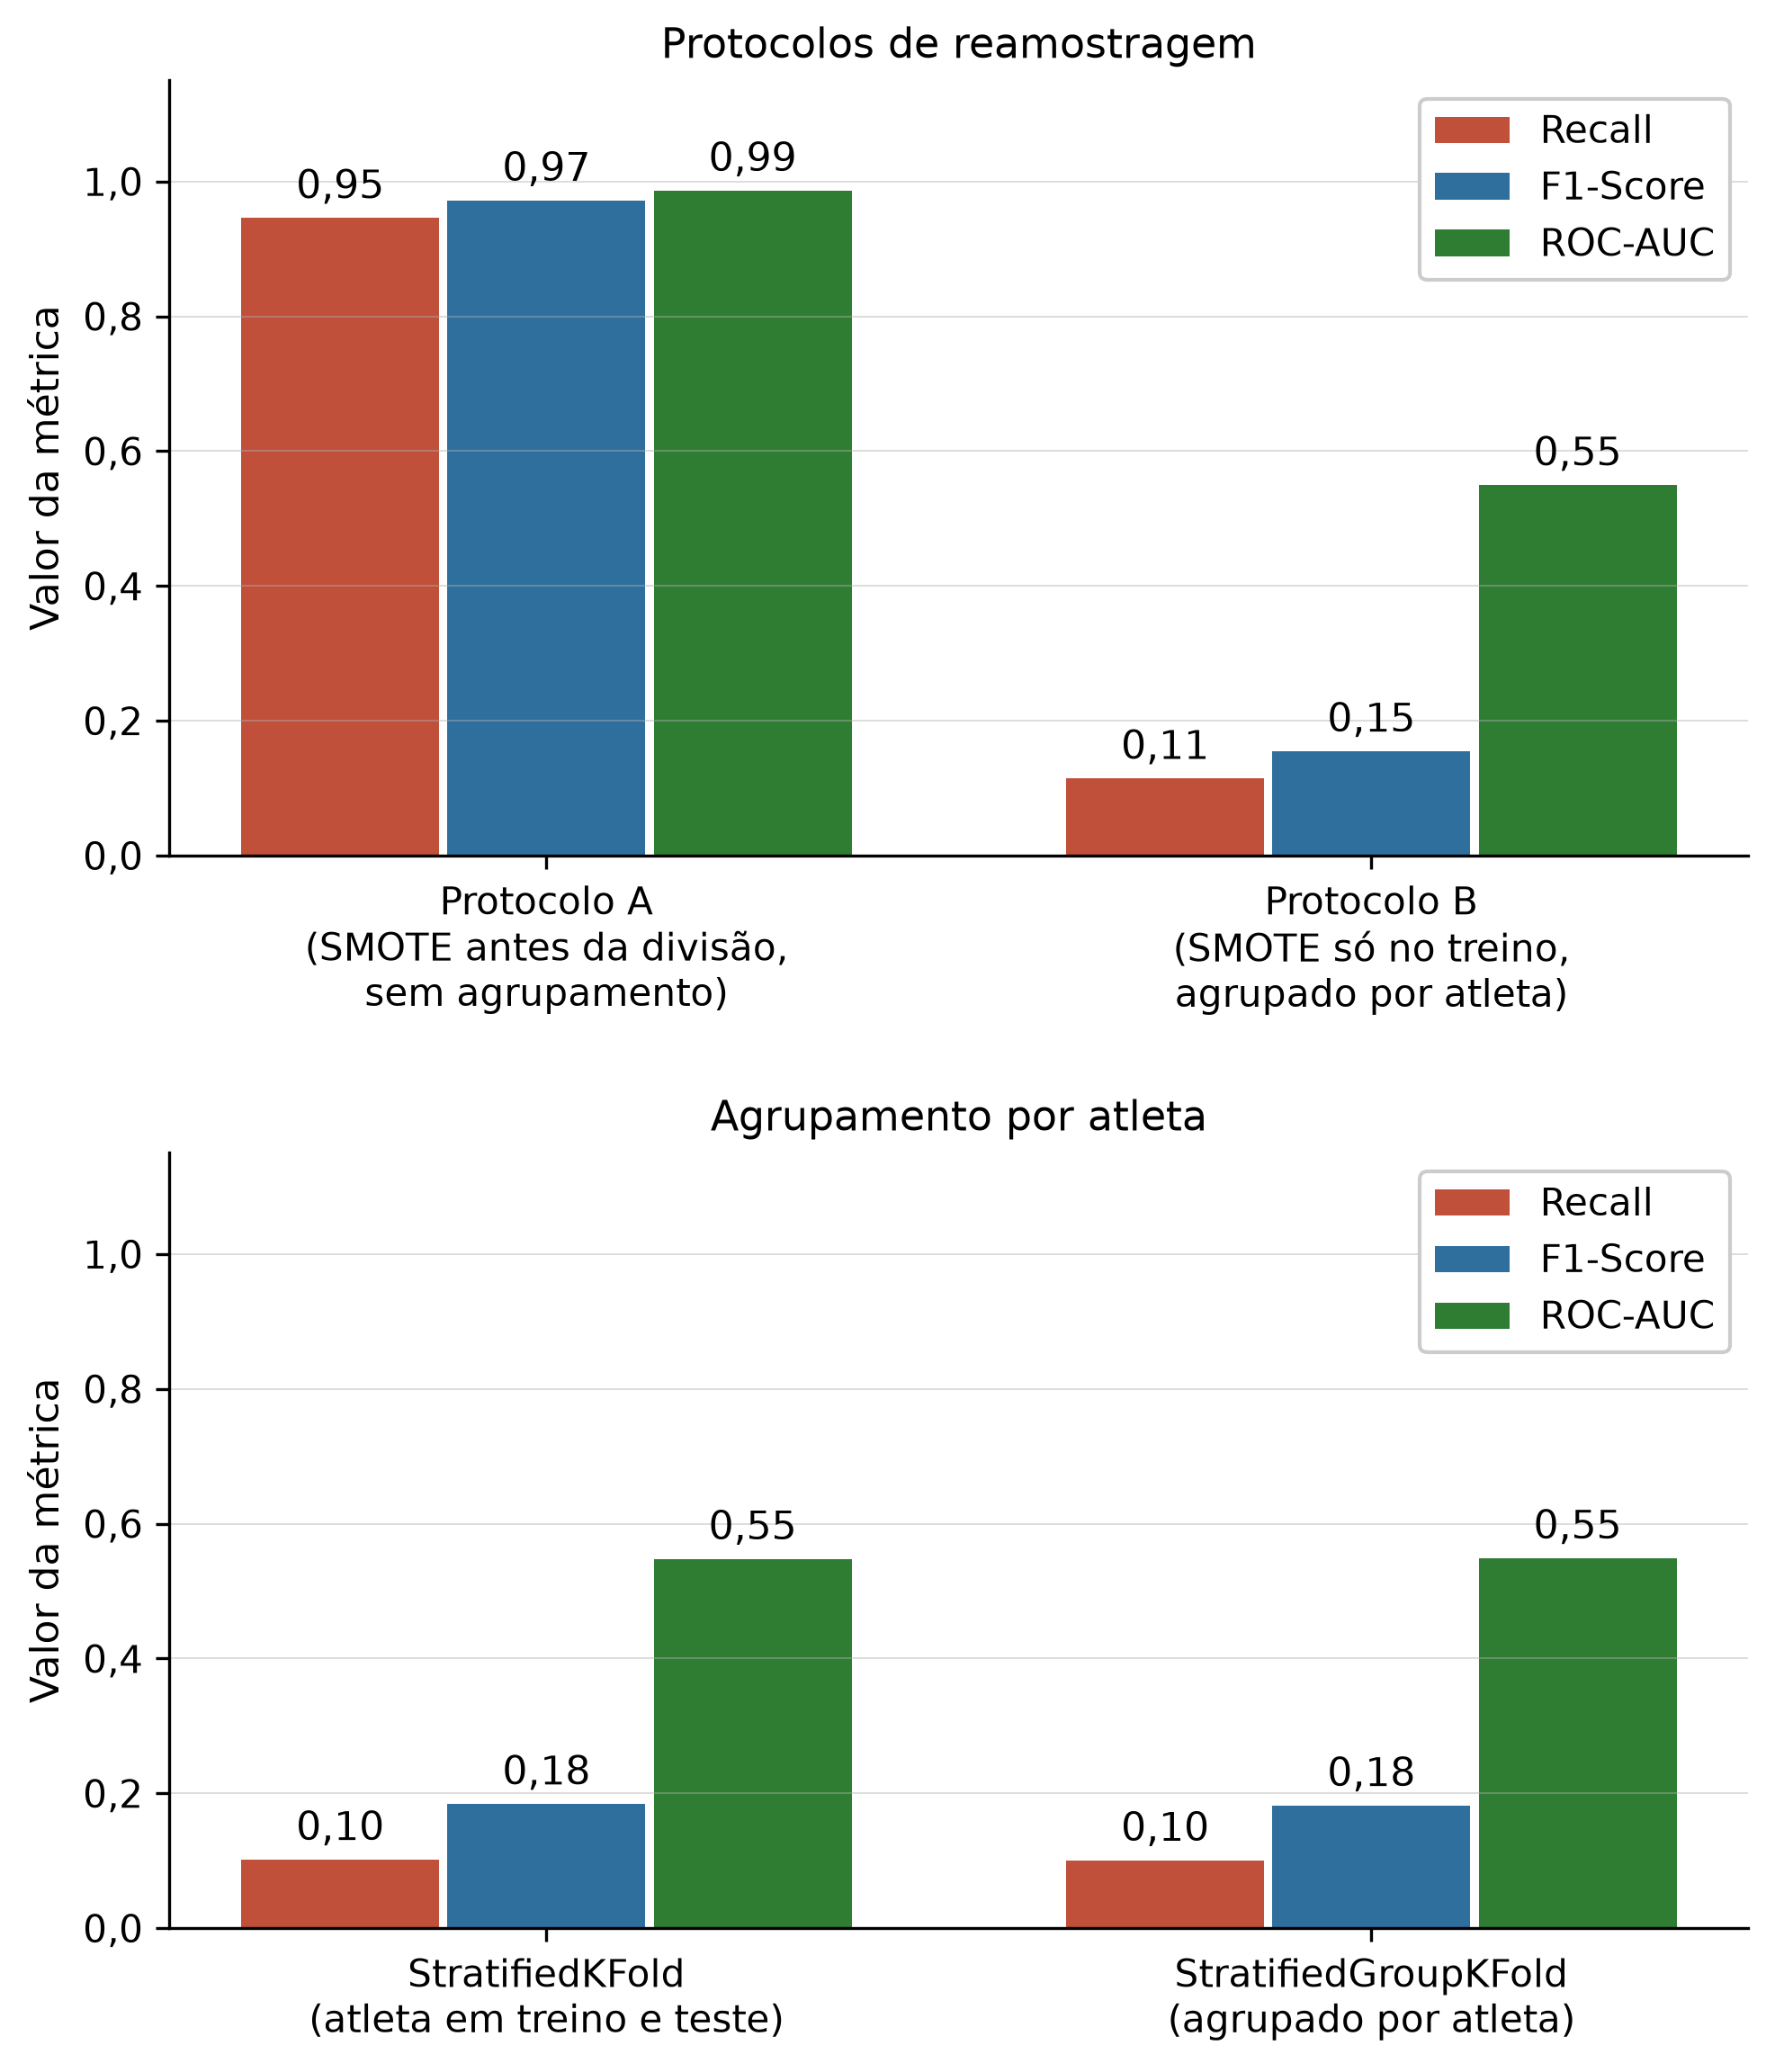
\includegraphics[width=\textwidth]{fig_leve/37_protocolos_validacao_v3.png}
    \caption{Métricas sob os protocolos comparados.}
    \label{fig:leakage}
\end{figure}

O painel superior da figura mostra os dois protocolos completos de reamostragem da Tabela~\ref{tab:protocolos_smote}, e o inferior, a validação sem e com agrupamento por atleta, examinada na subseção seguinte. Cabe precisar a atribuição do efeito observado no painel superior. Como a Tabela~\ref{tab:protocolos_smote} explicita, o protocolo A difere do protocolo B em três aspectos simultâneos, e o desenho adotado não permite isolar a contribuição de cada um. A distorção observada deve ser atribuída ao protocolo inadequado como um todo, e não exclusivamente ao vazamento de informação entre treino e teste. Isolar os componentes exigiria experimentos adicionais, nos quais cada diferença fosse introduzida separadamente. O que o resultado estabelece é que uma sequência de decisões aparentemente razoáveis, todas documentadas em tutoriais de uso corrente, produz métricas que não guardam relação com a capacidade preditiva dos dados.

\subsection{Agrupamento por Atleta}
A Tabela~\ref{tab:leakage_grupo} compara os dois protocolos de validação cruzada. Essa comparação responde a uma pergunta específica: se o desempenho medido se mantém quando o modelo é avaliado em atletas que não participaram do treinamento.

\begin{table}[H]
\centering
\caption{Efeito da sobreposição de atletas entre treino e teste.}
\label{tab:leakage_grupo}
\begin{tabular}{lrr}
\toprule
Protocolo & F1-Score & ROC-AUC \\
\midrule
StratifiedKFold (atleta vaza)    & 0{,}1842 & 0{,}5477 \\
StratifiedGroupKFold (correto)   & 0{,}1818 & 0{,}5488 \\
\addlinespace
Diferença & $-$0{,}0024 & $+$0{,}0011 \\
\bottomrule
\end{tabular}
\end{table}

Nesta base, a diferença foi pequena, inferior a $0{,}003$ em valor absoluto nas duas métricas, resultado compatível com rótulos que não dependem da identidade do atleta. Ainda assim, o protocolo agrupado foi mantido em todo o experimento: em dados de origem real, a sobreposição de atletas entre treino e teste pode produzir vazamento expressivo, e é tratada como falha de protocolo na revisão de Van Eetvelde et al. \cite{vaneetvelde2021}.

\section{Análise do Subconjunto de Futebol}
\label{sec:soccer}

Entre as bases públicas reunidas durante o levantamento havia um segundo arquivo, distribuído separadamente, contendo 5.100 registros de 51 atletas de futebol e apresentando as mesmas doze colunas da base principal. A intenção inicial era utilizá-lo como validação externa, isto é, repetir o experimento sobre dados independentes para verificar se os achados se sustentavam.

Essa intenção não se confirmou, porque uma verificação de procedência, conduzida por comparação registro a registro, estabeleceu que as 5.100 linhas desse arquivo aparecem de forma idêntica dentro da base principal. Os 51 atletas correspondem a 51 dos 234 atletas já presentes, e a base principal contém exatamente 5.100 registros cuja modalidade é futebol. O segundo arquivo é, portanto, um recorte da primeira base, e não uma coleta independente.

Essa constatação altera o estatuto do resultado: o que se obtém não é validação externa, e sim uma análise de subconjunto, isto é, a verificação de que os achados se mantêm quando a análise é restrita a uma única modalidade esportiva. A Tabela~\ref{tab:comparativo} apresenta a comparação sob esse enquadramento, lembrando que o subconjunto está contido na base completa.

\begin{table}[H]
\centering
\caption{Base completa e subconjunto de futebol.}
\label{tab:comparativo}
\begin{tabular}{lrr}
\toprule
Característica & Base completa & Subconjunto: futebol \\
\midrule
Registros                     & 23.400 & 5.100 \\
Atletas                       & 234    & 51 \\
Medições por atleta           & 100    & 100 \\
Modalidades                   & 5      & 1 \\
Proporção de casos de risco   & 5{,}54\% & 5{,}31\% \\
Registros abrangidos pela regra & 132  & 36 \\
Cobertura dos casos de risco  & 10{,}18\% & 13{,}28\% \\
Taxa de risco fora da regra & 5{,}01\% & 4{,}64\% \\
Maior tamanho de efeito no resíduo & 0{,}064 & 0{,}115 \\
F1-Score da regra na base inteira & 0{,}1847 & 0{,}2345 \\
F1-Score da regra nas partições & 0{,}1833 & 0{,}2299 \\
Melhor F1-Score obtido        & 0{,}1833 & 0{,}2222 \\
Melhor F1-Score sobre a regra nas partições & 100{,}0\% & 96{,}6\% \\
Diferença de recall entre protocolos de SMOTE & $+$0{,}83 & $+$0{,}84 \\
\bottomrule
\end{tabular}
\end{table}

Restrita ao futebol, a análise preserva os quatro achados principais. A regra permanece sem exceções, cobrindo 36 registros que são todos positivos. O melhor modelo alcança 96{,}6\% do F1-Score da regra nas mesmas partições. O protocolo inadequado de SMOTE produz diferença de magnitude equivalente. E as técnicas de explicabilidade apontam as mesmas duas variáveis. A diferença na cobertura, de 10{,}18\% na base completa para 13{,}28\% no subconjunto, decorre de os registros de futebol concentrarem proporcionalmente mais casos que satisfazem a regra, o que eleva o F1-Score da regra na base inteira de 0{,}1847 para 0{,}2345.

O alcance desse resultado é limitado: por se tratar de um recorte da mesma base, a consistência observada indica que os achados não dependem da mistura de modalidades, mas não constitui evidência de que se repetiriam em dados de outra procedência. A verificação em base genuinamente independente permanece como trabalho futuro.

% =====================================================================
% CAPÍTULO 6: CONCLUSÃO
% =====================================================================
\chapter{CONCLUSÃO}

Este trabalho investigou de que modo as características da rotulagem e os protocolos de validação afetam a avaliação de classificadores em uma base sintética de monitoramento esportivo. Os experimentos conduzidos sustentam três afirmações, apresentadas a seguir com as respectivas delimitações.

Quanto à rotulagem, a investigação identificou uma regra compatível com os rótulos observados. Registros com frequência cardíaca acima de 180 batimentos por minuto ou atividade muscular acima de 80\% recebem invariavelmente a marca de risco, sem nenhuma exceção entre os 132 casos nessa condição. Esses casos respondem por apenas 10{,}18\% das ocorrências de risco. Nos 89{,}82\% restantes, as análises conduzidas não identificaram sinal preditivo: além do tamanho de efeito desprezível, um \textit{Random Forest} treinado e avaliado exclusivamente nessa região, sob validação agrupada por atleta, obteve ROC-AUC de $0{,}4951$ e precisão média de $0{,}0506$, próxima da prevalência de $0{,}0501$. A base contém, portanto, uma parcela perfeitamente previsível e uma parcela sobre a qual os procedimentos empregados não encontraram estrutura aprendível, resultado compatível com uma componente aleatória de rotulagem.

Dessa estrutura decorre uma referência descritiva de F1-Score, condicionada à ausência de sinal no resíduo: $0{,}1847$ na base completa e $0{,}1833$ como média das mesmas dez partições usadas pelos modelos. O resultado central do trabalho diz respeito a essa regra: as 23.400 predições do \textit{Random Forest}, obtidas nas partições de teste, coincidiram com as classificações da regra de dois limiares identificada na base completa. Quando a busca pela regra foi repetida usando apenas os atletas de treinamento de cada partição, as mesmas duas variáveis foram recuperadas nas dez partições, e a regra redescoberta, aplicada aos atletas de teste, obteve F1 médio de 0{,}1831, próximo ao da regra de referência, de 0{,}1833. Nenhum dos modelos avaliados, incluindo os métodos de \textit{gradient boosting} e o \textit{Random Forest} com busca de hiperparâmetros, superou essa referência, e vários ficaram substancialmente abaixo dela.

A primeira ressalva a essas conclusões é que a regra foi identificada por inspeção da base completa, e a redescoberta dentro das partições, embora feita sem acesso aos atletas de teste, continua sendo uma verificação dentro da mesma base. A segunda é que o fato de nenhum dos algoritmos testados ter superado a referência não demonstra que nenhum outro modelo poderia fazê-lo.

Quanto aos protocolos de validação, dois desenhos frequentes foram comparados. Um protocolo que gera exemplos sintéticos da classe rara antes de separar os dados, e que com isso também altera a composição do conjunto de avaliação e dispensa o agrupamento por atleta, apresentou recall de 0{,}9459 e área sob a curva ROC de 0{,}9865, contra 0{,}1144 e 0{,}5497 do protocolo adequado. A diferença deve ser atribuída ao protocolo como um todo, e não a um único de seus componentes. Um experimento conduzido dessa forma reportaria desempenho quase perfeito sobre dados cuja parcela majoritária não apresentou sinal preditivo detectável. Permitir que medições de um mesmo atleta apareçam simultaneamente no treino e na avaliação, o que afeta a capacidade de generalizar para atletas não vistos, produziu nesta base diferença pequena, compatível com rótulos que não dependem da identidade do atleta; ainda assim, o protocolo conservador foi mantido, já que em dados de origem real a sobreposição tende a ser consequente.

A análise de explicabilidade, conduzida por três métodos, convergiu para as mesmas duas variáveis que compõem a regra. Essa convergência indica consistência entre os critérios internos do modelo e a regra identificada. Como ambas foram obtidas a partir da mesma amostra, não constitui validação independente do procedimento gerador, nem evidência de relação fisiológica entre as variáveis e o desfecho. No caso do SHAP, a subamostra utilizada continha um único registro da região da regra, e as diferenças de importância entre variáveis foram moderadas, de modo que esse resultado tem caráter exploratório e é a parte de menor peso da convergência.

A restrição da análise aos registros de uma única modalidade esportiva preservou todos os achados. Cabe registrar, contudo, que esse recorte está contido na base principal, de modo que o resultado caracteriza consistência interna e não validação sobre dados independentes.

Em síntese, três resultados se sustentam sobre a evidência reunida. Primeiro, a base contém uma regra compatível com a rotulagem, sem exceções na amostra examinada, cuja descoberta é descrita em detalhe e cujos limiares decorrem dos próprios dados. Segundo, as predições do \textit{Random Forest} coincidiram registro a registro com as da regra, que foi recuperada nas dez partições quando a busca usou apenas os atletas de treinamento, e nenhum dos modelos avaliados superou essa referência. Terceiro, um protocolo inadequado de reamostragem distorceu fortemente as métricas reportadas, produzindo indicadores próximos do desempenho perfeito sobre dados cuja parcela majoritária não apresentou sinal detectável.

A contribuição deste trabalho é a de um estudo de caso. Ele documenta um procedimento de auditoria de rotulagem aplicável a outras bases sintéticas, e quantifica, em um cenário concreto, a magnitude da distorção que decisões correntes de protocolo podem introduzir. A generalização desses achados a outras bases, outros domínios ou dados de origem real não é estabelecida aqui e permanece como questão em aberto.

\section{Limitações}

Os achados deste trabalho devem ser lidos à luz das seguintes limitações:
\begin{itemize}
    \item A base utilizada é sintética e não possui rotulagem verificada por profissionais de saúde. Os achados dizem respeito ao comportamento de classificadores e de protocolos de avaliação, e não à viabilidade clínica de monitoramento de atletas.
    \item Os achados foram obtidos sobre uma única base pública. A análise restrita aos registros de futebol não constitui replicação independente, por tratar-se de um recorte da mesma base.
    \item O estudo não incluiu arquiteturas de aprendizado profundo. Os métodos de \textit{gradient boosting} avaliados na Seção~\ref{sec:boosting} ficaram abaixo do \textit{Random Forest}, o que não sustenta a expectativa de que modelos de maior capacidade superem a referência derivada. Essa permanece, contudo, uma conjectura: o espaço de modelos não foi explorado de forma exaustiva, e a verificação continua pendente.
    \item A extensão dos achados a bases de monitoramento esportivo de origem real exige repetir o procedimento sobre dados coletados e rotulados por profissionais de saúde.
\end{itemize}

\section{Trabalhos Futuros}

Como desdobramentos deste trabalho, propõem-se as seguintes linhas de continuidade:
\begin{itemize}
    \item Retomar o escopo cardíaco originalmente concebido caso bases com rotulagem clínica validada em populações atléticas venham a se tornar acessíveis, aplicando o protocolo metodológico aqui consolidado.
    \item Replicar o protocolo experimental em \textit{datasets} com rotulagem clínica real para avaliar se os modelos conseguem capturar padrões fisiológicos genuínos.
    \item Avaliar arquiteturas de \textit{deep learning} sobre séries temporais fisiológicas completas, em vez da representação tabular por registro isolado adotada neste trabalho.
    \item Desenvolver um protótipo de monitoramento em tempo real para validação operacional dos classificadores em ambiente de campo.
\end{itemize}

% --- BIBLIOGRAFIA ---
\bibliographystyle{tcc-alpha}
\bibliography{refs_tcc}

\end{document}
